% !TeX program = lualatex
% ALIUS Bulletin native visual reconstruction source.
% Generated from off-repo reference layout data; does not include or input a pre-existing article PDF.
\ifdefined\ALIUSIssueBuild
\else
\documentclass{article}
\usepackage[paperwidth=612.0000bp,paperheight=792.0000bp,margin=0bp]{geometry}
\usepackage{graphicx}
\usepackage{xcolor}
\usepackage{tikz}
\usepackage{iftex}
\usepackage[hidelinks]{hyperref}
\ifPDFTeX
  \usepackage[T1]{fontenc}
  \usepackage[utf8]{inputenc}
  \usepackage{textcomp}
  \usepackage{amssymb}
\else
  \usepackage{fontspec}
\fi
\pagestyle{empty}
\fi
\ifPDFTeX
  \providecommand{\ALIUSDeclareUnicodeFallbacks}{%
    \DeclareUnicodeCharacter{00AC}{\ensuremath{\neg}}%
    \DeclareUnicodeCharacter{00BE}{\ensuremath{\frac{3}{4}}}%
    \DeclareUnicodeCharacter{0101}{\=a}%
    \DeclareUnicodeCharacter{0107}{\'c}%
    \DeclareUnicodeCharacter{012B}{\=\i}%
    \DeclareUnicodeCharacter{0131}{\i}%
    \DeclareUnicodeCharacter{0142}{\l}%
    \DeclareUnicodeCharacter{015B}{\'s}%
    \DeclareUnicodeCharacter{016B}{\=u}%
    \DeclareUnicodeCharacter{025C}{q}%
    \DeclareUnicodeCharacter{0278}{t}%
    \DeclareUnicodeCharacter{02AE}{Th}%
    \DeclareUnicodeCharacter{02B0}{ff}%
    \DeclareUnicodeCharacter{02B4}{ffi}%
    \DeclareUnicodeCharacter{02BE}{ft}%
    \DeclareUnicodeCharacter{02BF}{fi}%
    \DeclareUnicodeCharacter{02C0}{fl}%
    \DeclareUnicodeCharacter{02C1}{fi}%
    \DeclareUnicodeCharacter{02D9}{Th}%
    \DeclareUnicodeCharacter{02EF}{gy}%
    \DeclareUnicodeCharacter{0394}{\ensuremath{\Delta}}%
    \DeclareUnicodeCharacter{03B2}{\ensuremath{\beta}}%
    \DeclareUnicodeCharacter{03BA}{\ensuremath{\kappa}}%
    \DeclareUnicodeCharacter{068D}{-}%
    \DeclareUnicodeCharacter{08BC}{ti}%
    \DeclareUnicodeCharacter{099E}{ti}%
    \DeclareUnicodeCharacter{1E43}{\d{m}}%
    \DeclareUnicodeCharacter{1E47}{\d{n}}%
    \DeclareUnicodeCharacter{1E63}{\d{s}}%
    \DeclareUnicodeCharacter{201C}{``}%
    \DeclareUnicodeCharacter{201D}{''}%
    \DeclareUnicodeCharacter{2260}{\ensuremath{\neq}}%
    \DeclareUnicodeCharacter{25A1}{\ensuremath{\square}}%
  }%
  \ifdefined\ALIUSIssueBuild\else\ALIUSDeclareUnicodeFallbacks\fi
  \providecommand{\ALIUSFontLatoLight}{\fontfamily{lato-LF}\fontseries{l}\selectfont}
  \providecommand{\ALIUSFontLatoRegular}{\fontfamily{lato-LF}\fontseries{m}\selectfont}
  \providecommand{\ALIUSFontLatoItalic}{\fontfamily{lato-LF}\fontseries{m}\itshape}
  \providecommand{\ALIUSFontLatoLightItalic}{\fontfamily{lato-LF}\fontseries{l}\itshape}
  \providecommand{\ALIUSFontCormorantRegular}{\fontfamily{CormorantGaramond-LF}\fontseries{m}\selectfont}
  \providecommand{\ALIUSFontCormorantLight}{\fontfamily{CormorantGaramond-LF}\fontseries{l}\selectfont}
  \providecommand{\ALIUSFontCormorantMedium}{\fontfamily{CormorantGaramond-LF}\fontseries{medium}\selectfont}
  \providecommand{\ALIUSFontCormorantBold}{\fontfamily{CormorantGaramond-LF}\fontseries{b}\selectfont}
  \providecommand{\ALIUSFontCormorantItalic}{\fontfamily{CormorantGaramond-LF}\fontseries{m}\itshape}
  \providecommand{\ALIUSFontTimes}{\fontfamily{ptm}\selectfont}
  \providecommand{\ALIUSFontCalibri}{\fontfamily{phv}\selectfont}
  \providecommand{\ALIUSFontCambria}{\fontfamily{ptm}\selectfont}
  \providecommand{\ALIUSFontSymbolFallback}{\fontfamily{ptm}\selectfont}
\else
  \providecommand{\ALIUSFontLatoLight}{\fontspec{Lato Light}}
  \providecommand{\ALIUSFontLatoRegular}{\fontspec{Lato Regular}}
  \providecommand{\ALIUSFontLatoItalic}{\fontspec{Lato Italic}}
  \providecommand{\ALIUSFontLatoLightItalic}{\fontspec{Lato Light Italic}}
  \providecommand{\ALIUSFontCormorantRegular}{\fontspec{Cormorant Garamond Regular}}
  \providecommand{\ALIUSFontCormorantLight}{\fontspec{Cormorant Garamond Light}}
  \providecommand{\ALIUSFontCormorantMedium}{\fontspec{Cormorant Garamond Medium}}
  \providecommand{\ALIUSFontCormorantBold}{\fontspec{Cormorant Garamond Bold}}
  \providecommand{\ALIUSFontCormorantItalic}{\fontspec{Cormorant Garamond Italic}}
  \providecommand{\ALIUSFontTimes}{\fontspec{Times New Roman}}
  \providecommand{\ALIUSFontCalibri}{\fontspec{Calibri}}
  \providecommand{\ALIUSFontCambria}{\fontspec{Cambria}}
  \providecommand{\ALIUSFontSymbolFallback}{\fontspec{Times New Roman}}
\fi
\providecommand{\ALIUSPullQuoteOpen}{\textquotedblleft}
\providecommand{\ALIUSPullQuoteClose}{\textquotedblright}
\definecolor{ALIUSC000000}{HTML}{000000}
\definecolor{ALIUSC0000FF}{HTML}{0000FF}
\definecolor{ALIUSC1155CC}{HTML}{1155CC}
\definecolor{ALIUSC1F8135}{HTML}{1F8135}
\definecolor{ALIUSC595959}{HTML}{595959}
\definecolor{ALIUSC767171}{HTML}{767171}
\definecolor{ALIUSCBFBFBF}{HTML}{BFBFBF}
\definecolor{ALIUSCFFFFFF}{HTML}{FFFFFF}
\providecommand{\ALIUSPlacedText}[6]{%
  \node[anchor=north west,inner sep=0pt,outer sep=0pt,text=#4] at (#1bp,-#2bp) {%
    \resizebox{#3bp}{!}{{#5\fontsize{#6bp}{#6bp}\selectfont #6\kern0pt}}%
  };%
}
\providecommand{\ALIUSPlacedTextContent}[7]{%
  \node[anchor=north west,inner sep=0pt,outer sep=0pt,text=#4] at (#1bp,-#2bp) {%
    \resizebox{#3bp}{!}{{#5\fontsize{#6bp}{#6bp}\selectfont #7}}%
  };%
}
\ifdefined\ALIUSIssueBuild
\else
\begin{document}
\fi
% Page 1
\thispagestyle{empty}
\noindent\begin{tikzpicture}[remember picture,overlay,x=1bp,y=1bp,shift={(current page.north west)}]
  \fill[ALIUSC0000FF] (77.025bp,-352.350bp) rectangle ++(189.580bp,-0.250bp);
  \fill[ALIUSC1F8135] (403.680bp,-163.550bp) rectangle ++(99.525bp,-0.250bp);
  \fill[ALIUSC1F8135] (403.680bp,-245.330bp) rectangle ++(98.525bp,-0.250bp);
  \fill[ALIUSC1F8135] (403.180bp,-322.600bp) rectangle ++(115.550bp,-0.250bp);
  \fill[ALIUSC1F8135] (403.180bp,-402.120bp) rectangle ++(107.800bp,-0.250bp);
  \fill[ALIUSCBFBFBF] (398.180bp,-133.800bp) rectangle ++(0.500bp,-5.000bp);
  \fill[ALIUSCBFBFBF] (398.180bp,-138.790bp) rectangle ++(0.500bp,-292.330bp);
  \fill[ALIUSCFFFFFF] (398.180bp,-431.125bp) rectangle ++(257.600bp,-2.275bp);
  \ALIUSPlacedTextContent{72.025}{72.014}{475.063}{ALIUSC000000}{\ALIUSFontLatoRegular}{18.000}{The intimacy of psychedelics, language, and consciousness.}
  \ALIUSPlacedTextContent{72.025}{96.764}{284.521}{ALIUSC000000}{\ALIUSFontLatoLight}{18.000}{An interview with Jeremy I. Skipper}
  \ALIUSPlacedTextContent{403.680}{138.943}{82.836}{ALIUSC000000}{\ALIUSFontLatoRegular}{11.000}{Jeremy I Skipper}
  \ALIUSPlacedTextContent{403.680}{153.917}{101.824}{ALIUSC1F8135}{\ALIUSFontLatoRegular}{9.000}{jeremy.skipper@ucl.ac.uk}
  \ALIUSPlacedTextContent{403.680}{166.417}{138.366}{ALIUSC000000}{\ALIUSFontLatoLight}{9.000}{Division of Psychology \& Language}
  \ALIUSPlacedTextContent{403.680}{178.917}{155.574}{ALIUSC000000}{\ALIUSFontLatoLight}{9.000}{Sciences, University College of London,}
  \ALIUSPlacedTextContent{403.680}{191.197}{48.718}{ALIUSC000000}{\ALIUSFontLatoLight}{9.000}{London, UK}
  \ALIUSPlacedTextContent{403.680}{220.723}{71.586}{ALIUSC000000}{\ALIUSFontLatoRegular}{11.000}{Leor Roseman}
  \ALIUSPlacedTextContent{77.025}{228.749}{105.591}{ALIUSC000000}{\ALIUSFontLatoLight}{13.000}{By Leor Roseman}
  \ALIUSPlacedTextContent{403.680}{235.697}{100.824}{ALIUSC1F8135}{\ALIUSFontLatoRegular}{9.000}{L.Roseman@exeter.ac.uk}
  \ALIUSPlacedTextContent{77.025}{246.499}{188.861}{ALIUSC000000}{\ALIUSFontLatoLight}{13.000}{Transcribed by Matthieu Koroma}
  \ALIUSPlacedTextContent{403.680}{248.197}{106.468}{ALIUSC000000}{\ALIUSFontLatoLight}{9.000}{Department of Psychology}
  \ALIUSPlacedTextContent{403.680}{260.697}{81.718}{ALIUSC000000}{\ALIUSFontLatoLight}{9.000}{University of Exeter,}
  \ALIUSPlacedTextContent{77.025}{264.519}{248.641}{ALIUSC000000}{\ALIUSFontLatoLight}{13.000}{Edited by Matthieu Koroma \& George Fejer}
  \ALIUSPlacedTextContent{403.680}{272.967}{44.188}{ALIUSC000000}{\ALIUSFontLatoLight}{9.000}{Exeter, UK}
  \ALIUSPlacedTextContent{403.170}{297.993}{65.846}{ALIUSC000000}{\ALIUSFontLatoRegular}{11.000}{George Fejer}
  \ALIUSPlacedTextContent{77.025}{300.230}{309.005}{ALIUSC000000}{\ALIUSFontLatoLight}{10.000}{Cite as: Skipper, J., Fejer, G., Koroma, M., Roseman, L., (2024). The}
  \ALIUSPlacedTextContent{403.170}{312.967}{115.207}{ALIUSC1F8135}{\ALIUSFontLatoLight}{9.000}{george.fejer@uni-konstanz.de}
  \ALIUSPlacedTextContent{77.025}{313.980}{308.975}{ALIUSC000000}{\ALIUSFontLatoLight}{10.000}{intimacy of psychedelics, language, and consciousness. An interview}
  \ALIUSPlacedTextContent{403.170}{325.467}{85.728}{ALIUSC000000}{\ALIUSFontLatoLight}{9.000}{Cognitive Psychology}
  \ALIUSPlacedTextContent{77.025}{327.730}{308.810}{ALIUSC000000}{\ALIUSFontLatoLight}{10.000}{with Jeremy Skipper by Leor Roseman, ALIUS Bulletin, 6,}
  \ALIUSPlacedTextContent{77.025}{339.530}{195.000}{ALIUSC1F8135}{\ALIUSFontLatoLight}{10.000}{\href{https://doi.org/10.5281/zenodo.11091861}{https://doi.org/10.5281/zenodo.11091861}}
  \ALIUSPlacedTextContent{403.170}{337.967}{100.478}{ALIUSC000000}{\ALIUSFontLatoLight}{9.000}{University of Constance,}
  \ALIUSPlacedTextContent{403.170}{350.237}{78.228}{ALIUSC000000}{\ALIUSFontLatoLight}{9.000}{Konstanz, Germany}
  \ALIUSPlacedTextContent{401.420}{379.513}{88.440}{ALIUSC000000}{\ALIUSFontLatoRegular}{11.000}{Matthieu Koroma}
  \ALIUSPlacedTextContent{403.170}{392.487}{107.370}{ALIUSC1F8135}{\ALIUSFontLatoLight}{9.000}{matthieu.koroma@uliege.be}
  \ALIUSPlacedTextContent{403.680}{403.487}{109.498}{ALIUSC000000}{\ALIUSFontLatoLight}{9.000}{GIGA-CRC In Vivo Imaging}
  \ALIUSPlacedTextContent{403.680}{415.987}{108.405}{ALIUSC000000}{\ALIUSFontLatoLight}{9.000}{University of Liège, Belgium}
  \ALIUSPlacedTextContent{72.025}{433.332}{55.859}{ALIUSC000000}{\ALIUSFontLatoRegular}{14.000}{Abstract}
  \ALIUSPlacedTextContent{72.025}{464.793}{470.481}{ALIUSC000000}{\ALIUSFontLatoLight}{11.000}{This interview explores the intimate relationship between language and consciousness, drawing}
  \ALIUSPlacedTextContent{72.025}{480.043}{470.470}{ALIUSC000000}{\ALIUSFontLatoLight}{11.000}{insights from aphasia phenomenology, psychedelic experiences, and neuroscientific theories.}
  \ALIUSPlacedTextContent{72.025}{495.293}{470.672}{ALIUSC000000}{\ALIUSFontLatoLight}{11.000}{Jeremy I. Skipper, a cognitive neuroscientist, argues that language is not merely a tool for reporting}
  \ALIUSPlacedTextContent{72.025}{510.313}{470.492}{ALIUSC000000}{\ALIUSFontLatoLight}{11.000}{conscious experiences but plays a generative role in shaping and sustaining consciousness itself. He}
  \ALIUSPlacedTextContent{72.025}{525.563}{471.101}{ALIUSC000000}{\ALIUSFontLatoLight}{11.000}{critiques localizationist models of language processing, emphasizing the context-dependence and}
  \ALIUSPlacedTextContent{72.025}{540.813}{470.632}{ALIUSC000000}{\ALIUSFontLatoLight}{11.000}{dynamic recruitment of brain regions. Parallels are drawn between the experiences of aphasic}
  \ALIUSPlacedTextContent{72.025}{555.813}{470.839}{ALIUSC000000}{\ALIUSFontLatoLight}{11.000}{patients, who report a loss of self-narrative and increased connectedness, and the phenomenology}
  \ALIUSPlacedTextContent{72.025}{571.063}{471.158}{ALIUSC000000}{\ALIUSFontLatoLight}{11.000}{of psychedelic states, which often involve a dissolution of linguistic categories and a sense of}
  \ALIUSPlacedTextContent{72.025}{586.343}{470.536}{ALIUSC000000}{\ALIUSFontLatoLight}{11.000}{ineffability. Skipper outlines potential neural mechanisms linking language disruption to psychedelic}
  \ALIUSPlacedTextContent{72.025}{601.593}{471.132}{ALIUSC000000}{\ALIUSFontLatoLight}{11.000}{experiences and discusses the UNITy Project, aimed in part at studying post-acute meaning-making}
  \ALIUSPlacedTextContent{72.025}{616.593}{419.417}{ALIUSC000000}{\ALIUSFontLatoLight}{11.000}{processes and predicting changes in language and well-being after psychedelic sessions.}
  \ALIUSPlacedTextContent{72.025}{643.599}{46.851}{ALIUSC000000}{\ALIUSFontLatoItalic}{11.500}{Keywords}
  \ALIUSPlacedTextContent{118.800}{643.599}{2.726}{ALIUSC000000}{\ALIUSFontLatoLightItalic}{11.500}{:}
  \ALIUSPlacedTextContent{124.800}{643.599}{336.298}{ALIUSC000000}{\ALIUSFontLatoLightItalic}{11.500}{Language, Consciousness, Psychedelics, Neuroscience, Phenomenology}
  \ALIUSPlacedTextContent{72.025}{686.868}{470.470}{ALIUSC1F8135}{\ALIUSFontLatoRegular}{11.000}{Hello Jeremy. As a specialist in the neurobiology of language, your research explores the intricate}
  \ALIUSPlacedTextContent{72.025}{702.118}{470.283}{ALIUSC1F8135}{\ALIUSFontLatoRegular}{11.000}{relationship between language and consciousness, and you have recently launched the UNITy}
\end{tikzpicture}
\null
\newpage
% Page 2
\thispagestyle{empty}
\noindent\begin{tikzpicture}[remember picture,overlay,x=1bp,y=1bp,shift={(current page.north west)}]
  \fill[ALIUSC000000] (70.525bp,-56.530bp) rectangle ++(471.200bp,-0.500bp);
  \fill[ALIUSC000000] (70.525bp,-723.975bp) rectangle ++(471.200bp,-0.500bp);
  \ALIUSPlacedTextContent{72.025}{36.094}{376.171}{ALIUSC767171}{\ALIUSFontCormorantRegular}{14.000}{Skipper – The intimacy of psychedelics, language, and consciousness}
  \ALIUSPlacedTextContent{521.220}{38.866}{4.422}{ALIUSC000000}{\ALIUSFontCormorantRegular}{11.000}{2}
  \ALIUSPlacedTextContent{72.025}{72.173}{470.305}{ALIUSC1F8135}{\ALIUSFontLatoRegular}{11.000}{Project, short for Understanding Neuroplasticity Induced by Tryptamine, focusing on the effects}
  \ALIUSPlacedTextContent{72.025}{87.423}{470.547}{ALIUSC1F8135}{\ALIUSFontLatoRegular}{11.000}{of psychedelics on brain plasticity and language, among other things. I assume we will delve deeper}
  \ALIUSPlacedTextContent{72.025}{102.423}{343.711}{ALIUSC1F8135}{\ALIUSFontLatoRegular}{11.000}{into these topics. Could you start by telling us about your background?}
  \ALIUSPlacedTextContent{72.025}{137.114}{470.778}{ALIUSC000000}{\ALIUSFontCormorantRegular}{14.000}{I got into psychology because I wanted to figure out why I was always getting kicked}
  \ALIUSPlacedTextContent{72.025}{156.614}{471.301}{ALIUSC000000}{\ALIUSFontCormorantRegular}{14.000}{out of classes. I was in a gifted program and had all of my dreams come crashing down}
  \ALIUSPlacedTextContent{72.025}{176.114}{470.736}{ALIUSC000000}{\ALIUSFontCormorantRegular}{14.000}{when I was removed from it to be put into vocational school. I'm not diminishing}
  \ALIUSPlacedTextContent{72.025}{195.644}{471.345}{ALIUSC000000}{\ALIUSFontCormorantRegular}{14.000}{vocational schools as I learned to weld and it was super cool. I was a really bad student}
  \ALIUSPlacedTextContent{72.025}{215.144}{470.722}{ALIUSC000000}{\ALIUSFontCormorantRegular}{14.000}{and was told that I would never succeed because I couldn't think properly. It was a}
  \ALIUSPlacedTextContent{72.025}{234.644}{270.651}{ALIUSC000000}{\ALIUSFontCormorantRegular}{14.000}{shock to everybody that I graduated high school.}
  \ALIUSPlacedTextContent{72.025}{273.664}{470.820}{ALIUSC000000}{\ALIUSFontCormorantRegular}{14.000}{Only in my second year of college did I become interested in consciousness. That was}
  \ALIUSPlacedTextContent{72.025}{293.164}{470.778}{ALIUSC000000}{\ALIUSFontCormorantRegular}{14.000}{the cool thing that you talked about in high school and more in college, around the}
  \ALIUSPlacedTextContent{72.025}{312.664}{470.806}{ALIUSC000000}{\ALIUSFontCormorantRegular}{14.000}{campfire, and with your friends, and got high and said ridiculous things about}
  \ALIUSPlacedTextContent{72.025}{332.164}{470.785}{ALIUSC000000}{\ALIUSFontCormorantRegular}{14.000}{consciousness. That was what I was really jazzed about and why I went into science. I}
  \ALIUSPlacedTextContent{72.025}{351.684}{471.423}{ALIUSC000000}{\ALIUSFontCormorantRegular}{14.000}{started reading obsessively. But at the end of it, no way I would get into any grad school.}
  \ALIUSPlacedTextContent{72.025}{371.184}{471.481}{ALIUSC000000}{\ALIUSFontCormorantRegular}{14.000}{I didn't know if I wanted to do that. I cashed in all the bonds my grandmother gave me}
  \ALIUSPlacedTextContent{72.025}{390.684}{470.918}{ALIUSC000000}{\ALIUSFontCormorantRegular}{14.000}{when I was growing up and lived in a car with a guy for two years. During that time, I}
  \ALIUSPlacedTextContent{72.025}{410.184}{471.391}{ALIUSC000000}{\ALIUSFontCormorantRegular}{14.000}{read David Chalmers' (1997) The Conscious Mind and Dennett's (1993) Consciousness}
  \ALIUSPlacedTextContent{72.025}{429.714}{63.551}{ALIUSC000000}{\ALIUSFontCormorantRegular}{14.000}{Explained.}
  \ALIUSPlacedTextContent{72.025}{468.714}{470.974}{ALIUSC000000}{\ALIUSFontCormorantRegular}{14.000}{At the end of two years, I knew that I didn't want to live in a car anymore and wanted}
  \ALIUSPlacedTextContent{72.025}{488.214}{470.666}{ALIUSC000000}{\ALIUSFontCormorantRegular}{14.000}{to go to grad school. I was so excited about consciousness. I thought the way to get to}
  \ALIUSPlacedTextContent{72.025}{507.734}{471.463}{ALIUSC000000}{\ALIUSFontCormorantRegular}{14.000}{consciousness was to get there through studying the brain. I ended up in a program,}
  \ALIUSPlacedTextContent{72.025}{527.234}{471.044}{ALIUSC000000}{\ALIUSFontCormorantRegular}{14.000}{studied the brain, but ended up working on language, which isn't far removed. All of a}
  \ALIUSPlacedTextContent{72.025}{546.734}{471.055}{ALIUSC000000}{\ALIUSFontCormorantRegular}{14.000}{sudden, there is like a 20-year point where I'm very narrowly focused on this very}
  \ALIUSPlacedTextContent{72.025}{566.234}{471.467}{ALIUSC000000}{\ALIUSFontCormorantRegular}{14.000}{specific thing getting dumber and dumber and dumber as the years go by. Maybe there's}
  \ALIUSPlacedTextContent{72.025}{585.764}{470.680}{ALIUSC000000}{\ALIUSFontCormorantRegular}{14.000}{some thread that only the gods know about. I could probably make up a story, but I}
  \ALIUSPlacedTextContent{72.025}{605.264}{447.971}{ALIUSC000000}{\ALIUSFontCormorantRegular}{14.000}{think that it's almost serendipitously that I've been studying language for so long.}
  \ALIUSPlacedTextContent{72.025}{644.264}{470.829}{ALIUSC000000}{\ALIUSFontCormorantRegular}{14.000}{Recently I became unhappy with my position here and I started getting bored with}
  \ALIUSPlacedTextContent{72.025}{663.784}{471.469}{ALIUSC000000}{\ALIUSFontCormorantRegular}{14.000}{what I was doing. I thought that I needed to switch gears and change careers. I even}
  \ALIUSPlacedTextContent{72.025}{683.289}{471.273}{ALIUSC000000}{\ALIUSFontCormorantRegular}{14.000}{had a startup and tried different things like building sensory substitution devices for a}
  \ALIUSPlacedTextContent{72.025}{702.789}{471.487}{ALIUSC000000}{\ALIUSFontCormorantRegular}{14.000}{few years, and that didn't really work out. If I was going to stay in science, I wanted to}
  \ALIUSPlacedTextContent{72.025}{741.086}{112.024}{ALIUSC767171}{\ALIUSFontCormorantRegular}{11.000}{ALIUS Bulletin n°6 (2024)}
  \ALIUSPlacedTextContent{406.170}{741.086}{108.317}{ALIUSC1155CC}{\ALIUSFontCormorantRegular}{11.000}{aliusresearch.org/bulletin}
\end{tikzpicture}
\null
\newpage
% Page 3
\thispagestyle{empty}
\noindent\begin{tikzpicture}[remember picture,overlay,x=1bp,y=1bp,shift={(current page.north west)}]
  \fill[ALIUSC000000] (70.525bp,-56.530bp) rectangle ++(471.200bp,-0.500bp);
  \fill[ALIUSC000000] (70.525bp,-723.975bp) rectangle ++(471.200bp,-0.500bp);
  \ALIUSPlacedTextContent{72.025}{36.094}{376.171}{ALIUSC767171}{\ALIUSFontCormorantRegular}{14.000}{Skipper – The intimacy of psychedelics, language, and consciousness}
  \ALIUSPlacedTextContent{521.470}{38.866}{4.279}{ALIUSC000000}{\ALIUSFontCormorantRegular}{11.000}{3}
  \ALIUSPlacedTextContent{72.025}{72.094}{471.369}{ALIUSC000000}{\ALIUSFontCormorantRegular}{14.000}{go back to where I was when I was really excited. I thus started studying consciousness}
  \ALIUSPlacedTextContent{72.025}{91.594}{471.071}{ALIUSC000000}{\ALIUSFontCormorantRegular}{14.000}{again, which is the thing that I felt really compelled by around the campfire and in the}
  \ALIUSPlacedTextContent{72.025}{111.114}{470.848}{ALIUSC000000}{\ALIUSFontCormorantRegular}{14.000}{car. It has just changed my life. I was not unhappy before but I was not sure I was going}
  \ALIUSPlacedTextContent{72.025}{130.614}{470.991}{ALIUSC000000}{\ALIUSFontCormorantRegular}{14.000}{to stay in science and thought I really was on the verge of having some mental health}
  \ALIUSPlacedTextContent{72.025}{150.114}{60.051}{ALIUSC000000}{\ALIUSFontCormorantRegular}{14.000}{problems.}
  \ALIUSPlacedTextContent{72.025}{189.144}{470.722}{ALIUSC000000}{\ALIUSFontCormorantRegular}{14.000}{Sometimes I think it's interesting to talk about mental health and how it affects lives.}
  \ALIUSPlacedTextContent{72.025}{208.644}{470.778}{ALIUSC000000}{\ALIUSFontCormorantRegular}{14.000}{It is relevant only somewhat indirectly to the way I do research. I've always been into}
  \ALIUSPlacedTextContent{72.025}{228.144}{471.441}{ALIUSC000000}{\ALIUSFontCormorantRegular}{14.000}{psychedelic use personally because of some of the hypomania I've had. For example, I}
  \ALIUSPlacedTextContent{72.025}{247.644}{470.960}{ALIUSC000000}{\ALIUSFontCormorantRegular}{14.000}{didn't read at all until my second year of college when I started reading Tom Robbins.}
  \ALIUSPlacedTextContent{72.025}{267.164}{470.694}{ALIUSC000000}{\ALIUSFontCormorantRegular}{14.000}{Through him, I learned about Buddhism and how our categories mess up the way we}
  \ALIUSPlacedTextContent{72.025}{286.664}{471.481}{ALIUSC000000}{\ALIUSFontCormorantRegular}{14.000}{live. Then I started reading Alan Watts. Then I started reading obsessively at some}
  \ALIUSPlacedTextContent{72.025}{306.164}{211.131}{ALIUSC000000}{\ALIUSFontCormorantRegular}{14.000}{point, probably, 5 to 10 books a week.}
  \ALIUSPlacedTextContent{72.025}{345.184}{470.946}{ALIUSC000000}{\ALIUSFontCormorantRegular}{14.000}{Switching from zero reading to doing that in a process of ingesting so much so quickly}
  \ALIUSPlacedTextContent{72.025}{364.684}{470.764}{ALIUSC000000}{\ALIUSFontCormorantRegular}{14.000}{drove my interest in this idea of losing categories. Alan Watts does a nice job talking}
  \ALIUSPlacedTextContent{72.025}{384.184}{471.411}{ALIUSC000000}{\ALIUSFontCormorantRegular}{14.000}{about it, especially if you're an undergrad. I grew up in a very Christian household, my}
  \ALIUSPlacedTextContent{72.025}{403.684}{470.708}{ALIUSC000000}{\ALIUSFontCormorantRegular}{14.000}{mother is a lay preacher and I had very fixed ideas about what the world was until I}
  \ALIUSPlacedTextContent{72.025}{423.214}{470.722}{ALIUSC000000}{\ALIUSFontCormorantRegular}{14.000}{started reading these. I didn't get this from my education. Then I got obsessive about}
  \ALIUSPlacedTextContent{72.025}{442.714}{471.397}{ALIUSC000000}{\ALIUSFontCormorantRegular}{14.000}{it when I started doing psychedelics, as a way to explore those concepts. I think it's}
  \ALIUSPlacedTextContent{72.025}{462.214}{311.901}{ALIUSC000000}{\ALIUSFontCormorantRegular}{14.000}{probably true of everybody so it's not really that unique.}
  \ALIUSPlacedTextContent{72.025}{501.234}{470.806}{ALIUSC000000}{\ALIUSFontCormorantRegular}{14.000}{When I hopped back into it, I started looking into the neural correlates of}
  \ALIUSPlacedTextContent{72.025}{520.734}{470.918}{ALIUSC000000}{\ALIUSFontCormorantRegular}{14.000}{consciousness work. There is zero, maybe one mention and almost no discussion of the}
  \ALIUSPlacedTextContent{72.025}{540.234}{470.806}{ALIUSC000000}{\ALIUSFontCormorantRegular}{14.000}{relationship between language and consciousness. Yet, philosophically there has been,}
  \ALIUSPlacedTextContent{72.025}{559.734}{470.939}{ALIUSC000000}{\ALIUSFontCormorantRegular}{14.000}{and phenomenologically, we all think that there's a very strong connection somehow}
  \ALIUSPlacedTextContent{72.025}{579.264}{470.862}{ALIUSC000000}{\ALIUSFontCormorantRegular}{14.000}{between language and consciousness. Dan Dennett puts it in a nice way. Actually, he's}
  \ALIUSPlacedTextContent{72.025}{598.764}{470.750}{ALIUSC000000}{\ALIUSFontCormorantRegular}{14.000}{quoting somebody else who's quoting somebody else, going like: we think there's such}
  \ALIUSPlacedTextContent{72.025}{618.264}{471.039}{ALIUSC000000}{\ALIUSFontCormorantRegular}{14.000}{a strong connection because we don't notice that we're conscious about things that are}
  \ALIUSPlacedTextContent{72.025}{637.764}{470.820}{ALIUSC000000}{\ALIUSFontCormorantRegular}{14.000}{happening to us or within us until we verbalize it. We spend so much time doing it. I}
  \ALIUSPlacedTextContent{72.025}{657.284}{470.963}{ALIUSC000000}{\ALIUSFontCormorantRegular}{14.000}{thought, "Oh my god, there's a huge hole in the literature" in the neural correlates of}
  \ALIUSPlacedTextContent{72.025}{676.784}{385.701}{ALIUSC000000}{\ALIUSFontCormorantRegular}{14.000}{consciousness, which is quite comparable in the psychedelic literature.}
  \ALIUSPlacedTextContent{72.025}{741.086}{112.024}{ALIUSC767171}{\ALIUSFontCormorantRegular}{11.000}{ALIUS Bulletin n°6 (2024)}
  \ALIUSPlacedTextContent{406.170}{741.086}{108.317}{ALIUSC1155CC}{\ALIUSFontCormorantRegular}{11.000}{aliusresearch.org/bulletin}
\end{tikzpicture}
\null
\newpage
% Page 4
\thispagestyle{empty}
\noindent\begin{tikzpicture}[remember picture,overlay,x=1bp,y=1bp,shift={(current page.north west)}]
  \fill[ALIUSC000000] (70.525bp,-56.530bp) rectangle ++(471.200bp,-0.500bp);
  \fill[ALIUSC000000] (70.525bp,-723.975bp) rectangle ++(471.200bp,-0.500bp);
  \ALIUSPlacedTextContent{72.025}{36.094}{376.171}{ALIUSC767171}{\ALIUSFontCormorantRegular}{14.000}{Skipper – The intimacy of psychedelics, language, and consciousness}
  \ALIUSPlacedTextContent{520.720}{38.866}{4.961}{ALIUSC000000}{\ALIUSFontCormorantRegular}{11.000}{4}
  \ALIUSPlacedTextContent{72.025}{72.094}{471.021}{ALIUSC000000}{\ALIUSFontCormorantRegular}{14.000}{I said: "Okay, I really love psychedelics, and I really love consciousness. I'm going to use}
  \ALIUSPlacedTextContent{72.025}{91.594}{471.131}{ALIUSC000000}{\ALIUSFontCormorantRegular}{14.000}{psychedelics to perturb consciousness.". I already thought about this connection}
  \ALIUSPlacedTextContent{72.025}{111.114}{470.764}{ALIUSC000000}{\ALIUSFontCormorantRegular}{14.000}{between aphasia and people's descriptions of having their self mostly disappear and}
  \ALIUSPlacedTextContent{72.025}{130.614}{471.016}{ALIUSC000000}{\ALIUSFontCormorantRegular}{14.000}{having a stronger connection between them. I was maybe a little naive when I thought}
  \ALIUSPlacedTextContent{72.025}{150.114}{471.227}{ALIUSC000000}{\ALIUSFontCormorantRegular}{14.000}{about it but I think when I started, I would have said there was nothing about language,}
  \ALIUSPlacedTextContent{72.025}{169.614}{471.487}{ALIUSC000000}{\ALIUSFontCormorantRegular}{14.000}{the neurobiology of language, and work in the domain of psychedelics, and I wanted to}
  \ALIUSPlacedTextContent{72.025}{189.144}{470.722}{ALIUSC000000}{\ALIUSFontCormorantRegular}{14.000}{use that as a tool to perturb conscious experience because of that phenomenology of}
  \ALIUSPlacedTextContent{72.025}{208.644}{48.051}{ALIUSC000000}{\ALIUSFontCormorantRegular}{14.000}{oneness.}
  \ALIUSPlacedTextContent{72.025}{244.486}{342.717}{ALIUSC1F8135}{\ALIUSFontLatoRegular}{12.000}{I heard a rumor that you used to give talks barefoot. Is that true?}
  \ALIUSPlacedTextContent{165.830}{274.225}{14.167}{ALIUSC595959}{\ALIUSFontCormorantRegular}{48.025}{\ALIUSPullQuoteOpen}
  \ALIUSPlacedTextContent{190.080}{286.295}{247.995}{ALIUSC000000}{\ALIUSFontLatoLight}{15.000}{I've tried to adapt to my weirdness by}
  \ALIUSPlacedTextContent{415.670}{302.225}{14.167}{ALIUSC595959}{\ALIUSFontCormorantRegular}{48.025}{\ALIUSPullQuoteClose}
  \ALIUSPlacedTextContent{215.350}{307.045}{192.960}{ALIUSC000000}{\ALIUSFontLatoLight}{15.000}{becoming weirder sometimes.}
  \ALIUSPlacedTextContent{72.025}{356.184}{470.820}{ALIUSC000000}{\ALIUSFontCormorantRegular}{14.000}{That's entirely true. For 20 years in my life, I have had this weird phase in my life,}
  \ALIUSPlacedTextContent{72.025}{375.684}{471.291}{ALIUSC000000}{\ALIUSFontCormorantRegular}{14.000}{starting in my second year of college where I only wore flip-flops. I even gave my job}
  \ALIUSPlacedTextContent{72.025}{395.184}{471.425}{ALIUSC000000}{\ALIUSFontCormorantRegular}{14.000}{talk at UCL in a suit and flip-flops. I always wondered if I liked wearing flip-flops}
  \ALIUSPlacedTextContent{72.025}{414.684}{471.323}{ALIUSC000000}{\ALIUSFontCormorantRegular}{14.000}{because it made people engage with me: "Why are you wearing flip-flops in the snow}
  \ALIUSPlacedTextContent{72.025}{434.214}{471.055}{ALIUSC000000}{\ALIUSFontCormorantRegular}{14.000}{in Chicago when it's 30 below zero?" I've tried to adapt to my weirdness by becoming}
  \ALIUSPlacedTextContent{72.025}{453.714}{471.473}{ALIUSC000000}{\ALIUSFontCormorantRegular}{14.000}{weirder sometimes. I literally have no answer in my own head as to why I did that, and}
  \ALIUSPlacedTextContent{72.025}{473.214}{471.421}{ALIUSC000000}{\ALIUSFontCormorantRegular}{14.000}{I always make up a different story to the question "why do you wear flip-flops?". There}
  \ALIUSPlacedTextContent{72.025}{492.714}{316.151}{ALIUSC000000}{\ALIUSFontCormorantRegular}{14.000}{must be something I should talk about with my therapist.}
  \ALIUSPlacedTextContent{72.025}{528.826}{422.747}{ALIUSC1F8135}{\ALIUSFontLatoRegular}{12.000}{Has that weirdness manifested in your research and work as a scientist as well?}
  \ALIUSPlacedTextContent{72.025}{562.484}{470.974}{ALIUSC000000}{\ALIUSFontCormorantRegular}{14.000}{Thanks, yes for sure. There are two clear examples which we have already spoken about.}
  \ALIUSPlacedTextContent{72.025}{582.014}{470.778}{ALIUSC000000}{\ALIUSFontCormorantRegular}{14.000}{One is that from my basic science perspective, I study the neurobiology of language}
  \ALIUSPlacedTextContent{72.025}{601.514}{470.778}{ALIUSC000000}{\ALIUSFontCormorantRegular}{14.000}{and 99\% of the study of the neurobiology of languages is people putting people in}
  \ALIUSPlacedTextContent{72.025}{621.014}{470.951}{ALIUSC000000}{\ALIUSFontCormorantRegular}{14.000}{scanners and making them listen to speech sounds or single words. I really don't think}
  \ALIUSPlacedTextContent{72.025}{640.514}{470.778}{ALIUSC000000}{\ALIUSFontCormorantRegular}{14.000}{that's the only way to understand the neurobiology of language. It's probably in fact}
  \ALIUSPlacedTextContent{72.025}{660.044}{127.331}{ALIUSC000000}{\ALIUSFontCormorantRegular}{14.000}{one of the worst ways.}
  \ALIUSPlacedTextContent{72.025}{741.086}{112.024}{ALIUSC767171}{\ALIUSFontCormorantRegular}{11.000}{ALIUS Bulletin n°6 (2024)}
  \ALIUSPlacedTextContent{406.170}{741.086}{108.317}{ALIUSC1155CC}{\ALIUSFontCormorantRegular}{11.000}{aliusresearch.org/bulletin}
\end{tikzpicture}
\null
\newpage
% Page 5
\thispagestyle{empty}
\noindent\begin{tikzpicture}[remember picture,overlay,x=1bp,y=1bp,shift={(current page.north west)}]
  \fill[ALIUSC000000] (70.525bp,-56.530bp) rectangle ++(471.200bp,-0.500bp);
  \fill[ALIUSC000000] (70.525bp,-723.975bp) rectangle ++(471.200bp,-0.500bp);
  \ALIUSPlacedTextContent{72.025}{36.094}{376.171}{ALIUSC767171}{\ALIUSFontCormorantRegular}{14.000}{Skipper – The intimacy of psychedelics, language, and consciousness}
  \ALIUSPlacedTextContent{521.220}{38.866}{4.499}{ALIUSC000000}{\ALIUSFontCormorantRegular}{11.000}{5}
  \ALIUSPlacedTextContent{79.275}{79.198}{14.160}{ALIUSC595959}{\ALIUSFontCormorantRegular}{48.000}{\ALIUSPullQuoteOpen}
  \ALIUSPlacedTextContent{102.550}{89.200}{450.510}{ALIUSC000000}{\ALIUSFontLatoLight}{15.025}{I've always taken a little bit more tricky approach to the neurobiology}
  \ALIUSPlacedTextContent{133.300}{109.995}{389.160}{ALIUSC000000}{\ALIUSFontLatoLight}{15.000}{of language. We are using it right now, it is a conversational}
  \ALIUSPlacedTextContent{534.720}{126.675}{14.167}{ALIUSC595959}{\ALIUSFontCormorantRegular}{48.025}{\ALIUSPullQuoteClose}
  \ALIUSPlacedTextContent{144.050}{130.495}{364.095}{ALIUSC000000}{\ALIUSFontLatoLight}{15.000}{perspective, where we actually make use of the context.}
  \ALIUSPlacedTextContent{72.025}{183.394}{470.848}{ALIUSC000000}{\ALIUSFontCormorantRegular}{14.000}{I've always taken a little bit more tricky approach to the neurobiology of language. We}
  \ALIUSPlacedTextContent{72.025}{202.894}{470.834}{ALIUSC000000}{\ALIUSFontCormorantRegular}{14.000}{are using it right now, it is a conversational perspective, where we make use of the}
  \ALIUSPlacedTextContent{72.025}{222.394}{471.481}{ALIUSC000000}{\ALIUSFontCormorantRegular}{14.000}{context. From the very beginning of my career in 1999, I studied how the brain makes}
  \ALIUSPlacedTextContent{72.025}{241.894}{470.778}{ALIUSC000000}{\ALIUSFontCormorantRegular}{14.000}{use of context. My first study putting people in a scanner was having them listen to}
  \ALIUSPlacedTextContent{72.025}{261.414}{470.904}{ALIUSC000000}{\ALIUSFontCormorantRegular}{14.000}{videos, and movies of me telling stories about my life recorded from the head up. One}
  \ALIUSPlacedTextContent{72.025}{280.914}{471.445}{ALIUSC000000}{\ALIUSFontCormorantRegular}{14.000}{of the stories is about how I used to get naked and sit in the new fountain that we got}
  \ALIUSPlacedTextContent{72.025}{300.414}{470.876}{ALIUSC000000}{\ALIUSFontCormorantRegular}{14.000}{on my campus, in North Carolina during the summers. I spent quite a number of years}
  \ALIUSPlacedTextContent{72.025}{319.914}{471.051}{ALIUSC000000}{\ALIUSFontCormorantRegular}{14.000}{trying to understand the visual context, if the brain makes use of gestures that people}
  \ALIUSPlacedTextContent{72.025}{339.414}{471.215}{ALIUSC000000}{\ALIUSFontCormorantRegular}{14.000}{produce with their hands, mouth movements, and posture, and how we use that}
  \ALIUSPlacedTextContent{72.025}{358.934}{470.918}{ALIUSC000000}{\ALIUSFontCormorantRegular}{14.000}{information to help us comprehend the words that people are saying. My approach was}
  \ALIUSPlacedTextContent{72.025}{378.434}{470.792}{ALIUSC000000}{\ALIUSFontCormorantRegular}{14.000}{always to try to study language as a whole and try to reconstruct how the brain}
  \ALIUSPlacedTextContent{72.025}{397.934}{471.291}{ALIUSC000000}{\ALIUSFontCormorantRegular}{14.000}{processes all of the individual putative levels of analysis like phonemes, semantics,}
  \ALIUSPlacedTextContent{72.025}{417.434}{244.381}{ALIUSC000000}{\ALIUSFontCormorantRegular}{14.000}{speech production, attention, memory, etc…}
  \ALIUSPlacedTextContent{72.025}{451.306}{471.083}{ALIUSC1F8135}{\ALIUSFontLatoRegular}{12.000}{What findings did you make from the perspective of context dependency of language}
  \ALIUSPlacedTextContent{72.025}{467.806}{64.597}{ALIUSC1F8135}{\ALIUSFontLatoRegular}{12.000}{processing?}
  \ALIUSPlacedTextContent{72.025}{501.484}{470.666}{ALIUSC000000}{\ALIUSFontCormorantRegular}{14.000}{Philosophically or ideologically, I do not think you can study language outside of the}
  \ALIUSPlacedTextContent{72.025}{520.984}{470.974}{ALIUSC000000}{\ALIUSFontCormorantRegular}{14.000}{context of its use. I think it is misguided to start with the very fundamental assumption}
  \ALIUSPlacedTextContent{72.025}{540.484}{471.457}{ALIUSC000000}{\ALIUSFontCormorantRegular}{14.000}{that phonemes and words have any psychological reality in the brain. I can remember}
  \ALIUSPlacedTextContent{72.025}{559.984}{470.736}{ALIUSC000000}{\ALIUSFontCormorantRegular}{14.000}{this really fun meeting in Indiana with a guy named Robert Port at the end of his}
  \ALIUSPlacedTextContent{72.025}{579.514}{471.002}{ALIUSC000000}{\ALIUSFontCormorantRegular}{14.000}{career. He spent his whole life studying speech sounds trying to understand phonemes:}
  \ALIUSPlacedTextContent{72.025}{599.014}{470.876}{ALIUSC000000}{\ALIUSFontCormorantRegular}{14.000}{"what makes a phoneme a phoneme? How do you understand a phoneme? And how do}
  \ALIUSPlacedTextContent{72.025}{618.514}{470.805}{ALIUSC000000}{\ALIUSFontCormorantRegular}{14.000}{I understand the same phoneme as a phoneme? There must be some stable acoustic}
  \ALIUSPlacedTextContent{72.025}{638.014}{470.750}{ALIUSC000000}{\ALIUSFontCormorantRegular}{14.000}{properties of phonemes that allow you and me to understand the same thing when I}
  \ALIUSPlacedTextContent{72.025}{657.534}{20.020}{ALIUSC000000}{\ALIUSFontCormorantRegular}{14.000}{say}
  \ALIUSPlacedTextContent{94.300}{657.534}{17.094}{ALIUSC000000}{\ALIUSFontCormorantRegular}{14.000}{dog}
  \ALIUSPlacedTextContent{111.300}{657.534}{431.780}{ALIUSC000000}{\ALIUSFontCormorantRegular}{14.000}{". At the end of a 50-year career, he actually told me that he decided that}
  \ALIUSPlacedTextContent{72.025}{677.034}{470.736}{ALIUSC000000}{\ALIUSFontCormorantRegular}{14.000}{phonemes weren't real and had no psychological reality outside of the context of}
  \ALIUSPlacedTextContent{72.025}{696.539}{47.301}{ALIUSC000000}{\ALIUSFontCormorantRegular}{14.000}{reading.}
  \ALIUSPlacedTextContent{72.025}{741.086}{112.024}{ALIUSC767171}{\ALIUSFontCormorantRegular}{11.000}{ALIUS Bulletin n°6 (2024)}
  \ALIUSPlacedTextContent{406.170}{741.086}{108.317}{ALIUSC1155CC}{\ALIUSFontCormorantRegular}{11.000}{aliusresearch.org/bulletin}
\end{tikzpicture}
\null
\newpage
% Page 6
\thispagestyle{empty}
\noindent\begin{tikzpicture}[remember picture,overlay,x=1bp,y=1bp,shift={(current page.north west)}]
  \fill[ALIUSC000000] (70.525bp,-56.530bp) rectangle ++(471.200bp,-0.500bp);
  \fill[ALIUSC000000] (70.525bp,-723.975bp) rectangle ++(471.200bp,-0.500bp);
  \ALIUSPlacedTextContent{72.025}{36.094}{376.171}{ALIUSC767171}{\ALIUSFontCormorantRegular}{14.000}{Skipper – The intimacy of psychedelics, language, and consciousness}
  \ALIUSPlacedTextContent{520.720}{38.866}{5.115}{ALIUSC000000}{\ALIUSFontCormorantRegular}{11.000}{6}
  \ALIUSPlacedTextContent{99.800}{86.948}{14.160}{ALIUSC595959}{\ALIUSFontCormorantRegular}{48.000}{\ALIUSPullQuoteOpen}
  \ALIUSPlacedTextContent{125.550}{100.700}{346.882}{ALIUSC000000}{\ALIUSFontLatoLight}{15.025}{A really interesting way of thinking about speech and}
  \ALIUSPlacedTextContent{176.330}{121.245}{240.915}{ALIUSC000000}{\ALIUSFontLatoLight}{15.000}{language is that it is a grand delusion.}
  \ALIUSPlacedTextContent{470.950}{122.925}{14.167}{ALIUSC595959}{\ALIUSFontCormorantRegular}{48.025}{\ALIUSPullQuoteClose}
  \ALIUSPlacedTextContent{72.025}{174.364}{470.806}{ALIUSC000000}{\ALIUSFontCormorantRegular}{14.000}{A really interesting way of thinking about speech and language is that it is a grand}
  \ALIUSPlacedTextContent{72.025}{193.894}{90.860}{ALIUSC000000}{\ALIUSFontCormorantRegular}{14.000}{illusion. Imagine}
  \ALIUSPlacedTextContent{166.330}{193.894}{376.670}{ALIUSC000000}{\ALIUSFontCormorantRegular}{14.000}{hearing a language that is not a Romance language for the first time.}
  \ALIUSPlacedTextContent{72.025}{213.394}{470.946}{ALIUSC000000}{\ALIUSFontCormorantRegular}{14.000}{It sounds like a continuous stream of gibberish. If you do not understand anything and}
  \ALIUSPlacedTextContent{72.025}{232.894}{470.862}{ALIUSC000000}{\ALIUSFontCormorantRegular}{14.000}{there is nothing conveyed in any other channel, you have to kind of drop to the speech}
  \ALIUSPlacedTextContent{72.025}{252.394}{470.937}{ALIUSC000000}{\ALIUSFontCormorantRegular}{14.000}{level. But when you think consciously about what you're hearing, you hear words,}
  \ALIUSPlacedTextContent{72.025}{271.914}{471.481}{ALIUSC000000}{\ALIUSFontCormorantRegular}{14.000}{maybe sentences, and even sometimes phonemes. The reason I bring this up is that, i)}
  \ALIUSPlacedTextContent{72.025}{291.414}{447.471}{ALIUSC000000}{\ALIUSFontCormorantRegular}{14.000}{it makes speech and language interesting because it is a construction in our head,}
  \ALIUSPlacedTextContent{72.025}{310.914}{366.921}{ALIUSC000000}{\ALIUSFontCormorantRegular}{14.000}{and ii), it makes clear that we use different cues at different times.}
  \ALIUSPlacedTextContent{72.025}{349.934}{470.778}{ALIUSC000000}{\ALIUSFontCormorantRegular}{14.000}{I thus do not think that we have settled yet on the very fundamental components of}
  \ALIUSPlacedTextContent{72.025}{369.434}{470.876}{ALIUSC000000}{\ALIUSFontCormorantRegular}{14.000}{speech and language. With the reductionist approach, stimuli need to be very tightly}
  \ALIUSPlacedTextContent{72.025}{388.934}{471.279}{ALIUSC000000}{\ALIUSFontCormorantRegular}{14.000}{controlled by people pressing a button in a three-alternative forced choice task}
  \ALIUSPlacedTextContent{72.025}{408.434}{470.819}{ALIUSC000000}{\ALIUSFontCormorantRegular}{14.000}{comparing phonemes such as "PA", "KA", "TA". The assumption is that phonemes are}
  \ALIUSPlacedTextContent{72.025}{427.964}{470.960}{ALIUSC000000}{\ALIUSFontCormorantRegular}{14.000}{such a thing that can be studied outside of the context of the rest of language and that}
  \ALIUSPlacedTextContent{72.025}{447.464}{470.876}{ALIUSC000000}{\ALIUSFontCormorantRegular}{14.000}{it is going to tell you something meaningful about the neurobiology of language. I don't}
  \ALIUSPlacedTextContent{72.025}{466.964}{470.887}{ALIUSC000000}{\ALIUSFontCormorantRegular}{14.000}{think this to be true because of the ambiguity in speech sounds and a lack of invariance}
  \ALIUSPlacedTextContent{72.025}{486.464}{470.862}{ALIUSC000000}{\ALIUSFontCormorantRegular}{14.000}{that is found at all levels of analysis on which we have described language. At the}
  \ALIUSPlacedTextContent{72.025}{505.984}{470.806}{ALIUSC000000}{\ALIUSFontCormorantRegular}{14.000}{semantic level, words are polysemic and most words have at least five meanings. At}
  \ALIUSPlacedTextContent{72.025}{525.484}{471.037}{ALIUSC000000}{\ALIUSFontCormorantRegular}{14.000}{discourse level, there's clear ambiguity in the way sentences are formed and understood.}
  \ALIUSPlacedTextContent{72.025}{544.984}{312.151}{ALIUSC000000}{\ALIUSFontCormorantRegular}{14.000}{How does the brain overcome those levels of ambiguity?}
  \ALIUSPlacedTextContent{72.025}{584.014}{471.016}{ALIUSC000000}{\ALIUSFontCormorantRegular}{14.000}{I think the way that it does it is that we don't have divisibles. We don't have individual}
  \ALIUSPlacedTextContent{72.025}{603.514}{470.764}{ALIUSC000000}{\ALIUSFontCormorantRegular}{14.000}{speech sounds, words, and sentences but always use language in context. We always}
  \ALIUSPlacedTextContent{72.025}{623.014}{471.479}{ALIUSC000000}{\ALIUSFontCormorantRegular}{14.000}{have cues as to how a specific speech sound should be interpreted and are almost never}
  \ALIUSPlacedTextContent{72.025}{642.514}{470.946}{ALIUSC000000}{\ALIUSFontCormorantRegular}{14.000}{in the dark about that. The way that we have studied speech and language has actually}
  \ALIUSPlacedTextContent{72.025}{662.034}{470.974}{ALIUSC000000}{\ALIUSFontCormorantRegular}{14.000}{created this issue that maybe doesn't exist, the issue of ambiguity. In context, I can see}
  \ALIUSPlacedTextContent{72.025}{681.539}{471.399}{ALIUSC000000}{\ALIUSFontCormorantRegular}{14.000}{your lips when you're talking to me which helps me decode my speech sounds, and your}
  \ALIUSPlacedTextContent{72.025}{701.039}{470.876}{ALIUSC000000}{\ALIUSFontCormorantRegular}{14.000}{gestures which have semantic meaning that help me to decode what you're trying to}
  \ALIUSPlacedTextContent{72.025}{741.086}{112.024}{ALIUSC767171}{\ALIUSFontCormorantRegular}{11.000}{ALIUS Bulletin n°6 (2024)}
  \ALIUSPlacedTextContent{406.170}{741.086}{108.317}{ALIUSC1155CC}{\ALIUSFontCormorantRegular}{11.000}{aliusresearch.org/bulletin}
\end{tikzpicture}
\null
\newpage
% Page 7
\thispagestyle{empty}
\noindent\begin{tikzpicture}[remember picture,overlay,x=1bp,y=1bp,shift={(current page.north west)}]
  \fill[ALIUSC000000] (70.525bp,-56.530bp) rectangle ++(471.200bp,-0.500bp);
  \fill[ALIUSC000000] (70.525bp,-723.975bp) rectangle ++(471.200bp,-0.500bp);
  \ALIUSPlacedTextContent{72.025}{36.094}{376.171}{ALIUSC767171}{\ALIUSFontCormorantRegular}{14.000}{Skipper – The intimacy of psychedelics, language, and consciousness}
  \ALIUSPlacedTextContent{520.980}{38.866}{4.719}{ALIUSC000000}{\ALIUSFontCormorantRegular}{11.000}{7}
  \ALIUSPlacedTextContent{72.025}{72.094}{470.750}{ALIUSC000000}{\ALIUSFontCormorantRegular}{14.000}{say, I know you and have some background knowledge to help decode what you're}
  \ALIUSPlacedTextContent{72.025}{91.594}{40.278}{ALIUSC000000}{\ALIUSFontCormorantRegular}{14.000}{saying,}
  \ALIUSPlacedTextContent{111.800}{91.594}{16.492}{ALIUSC000000}{\ALIUSFontCormorantRegular}{14.000}{etc.}
  \ALIUSPlacedTextContent{128.300}{91.594}{6.276}{ALIUSC000000}{\ALIUSFontCormorantRegular}{14.000}{,}
  \ALIUSPlacedTextContent{134.050}{91.594}{13.818}{ALIUSC000000}{\ALIUSFontCormorantRegular}{14.000}{etc}
  \ALIUSPlacedTextContent{147.800}{91.594}{57.232}{ALIUSC000000}{\ALIUSFontCormorantRegular}{14.000}{., like that}
  \ALIUSPlacedTextContent{204.580}{91.594}{58.478}{ALIUSC000000}{\ALIUSFontCormorantRegular}{14.000}{ad nauseam}
  \ALIUSPlacedTextContent{263.100}{91.594}{280.084}{ALIUSC000000}{\ALIUSFontCormorantRegular}{14.000}{. To understand how people understand each other,}
  \ALIUSPlacedTextContent{72.025}{111.114}{470.988}{ALIUSC000000}{\ALIUSFontCormorantRegular}{14.000}{we need to study language in the context in which we use it because context is the only}
  \ALIUSPlacedTextContent{72.025}{130.614}{280.651}{ALIUSC000000}{\ALIUSFontCormorantRegular}{14.000}{place where language can be understood naturally.}
  \ALIUSPlacedTextContent{72.025}{169.614}{470.834}{ALIUSC000000}{\ALIUSFontCormorantRegular}{14.000}{I think there's room for pluralism of science here for people who study individual}
  \ALIUSPlacedTextContent{72.025}{189.144}{470.806}{ALIUSC000000}{\ALIUSFontCormorantRegular}{14.000}{speech sounds or individual words, and there needs to be people who study language}
  \ALIUSPlacedTextContent{72.025}{208.644}{470.862}{ALIUSC000000}{\ALIUSFontCormorantRegular}{14.000}{completely in context. I've attempted to do that at various levels of reductionism}
  \ALIUSPlacedTextContent{72.025}{228.144}{470.839}{ALIUSC000000}{\ALIUSFontCormorantRegular}{14.000}{myself, but I have also done speech sound studies or with podcasts or movies where we}
  \ALIUSPlacedTextContent{72.025}{247.644}{470.792}{ALIUSC000000}{\ALIUSFontCormorantRegular}{14.000}{try to construct how the brain does speech and language comprehension from the}
  \ALIUSPlacedTextContent{72.025}{267.164}{470.806}{ALIUSC000000}{\ALIUSFontCormorantRegular}{14.000}{activity patterns that we see, making no assumptions about what the levels and units}
  \ALIUSPlacedTextContent{72.025}{286.664}{470.891}{ALIUSC000000}{\ALIUSFontCormorantRegular}{14.000}{of analysis are. I think some of the things we found may be obvious and some of them}
  \ALIUSPlacedTextContent{72.025}{306.164}{241.631}{ALIUSC000000}{\ALIUSFontCormorantRegular}{14.000}{are yet to be answered and are not obvious.}
  \ALIUSPlacedTextContent{72.025}{342.434}{470.806}{ALIUSC000000}{\ALIUSFontCormorantRegular}{14.000}{One of the obvious things that we had to establish first is that the brain uses all the}
  \ALIUSPlacedTextContent{72.025}{361.934}{470.932}{ALIUSC000000}{\ALIUSFontCormorantRegular}{14.000}{context. People use gestures or mouth movements, even when they're not visible, which}
  \ALIUSPlacedTextContent{72.025}{381.434}{471.467}{ALIUSC000000}{\ALIUSFontCormorantRegular}{14.000}{is something weird. Prosody is the aspect of speech that involves variations in pitch,}
  \ALIUSPlacedTextContent{72.025}{400.934}{470.904}{ALIUSC000000}{\ALIUSFontCormorantRegular}{14.000}{rhythm, and intonation to convey meaning and emotional nuances. People use prosody}
  \ALIUSPlacedTextContent{72.025}{420.464}{470.792}{ALIUSC000000}{\ALIUSFontCormorantRegular}{14.000}{more or less depending on prior words. When people have some background about}
  \ALIUSPlacedTextContent{72.025}{439.964}{470.834}{ALIUSC000000}{\ALIUSFontCormorantRegular}{14.000}{what I am saying, people use this prior information at every given moment. We know}
  \ALIUSPlacedTextContent{72.025}{459.464}{470.823}{ALIUSC000000}{\ALIUSFontCormorantRegular}{14.000}{from individual studies that the brain uses all of these and now we're starting to learn}
  \ALIUSPlacedTextContent{72.025}{478.964}{470.764}{ALIUSC000000}{\ALIUSFontCormorantRegular}{14.000}{that the brain uses them all simultaneously, and more or less so depending on how}
  \ALIUSPlacedTextContent{72.025}{498.494}{470.904}{ALIUSC000000}{\ALIUSFontCormorantRegular}{14.000}{informative they are. You can have an extremely informative gesture that might tell}
  \ALIUSPlacedTextContent{72.025}{517.984}{470.871}{ALIUSC000000}{\ALIUSFontCormorantRegular}{14.000}{you something about people's semantic state or their emotional state and}
  \ALIUSPlacedTextContent{72.025}{537.484}{471.495}{ALIUSC000000}{\ALIUSFontCormorantRegular}{14.000}{uninformative prosody. There is thus a continually changing dynamic trade-off}
  \ALIUSPlacedTextContent{72.025}{556.984}{187.601}{ALIUSC000000}{\ALIUSFontCormorantRegular}{14.000}{between the cues that people use.}
  \ALIUSPlacedTextContent{72.025}{596.014}{470.932}{ALIUSC000000}{\ALIUSFontCormorantRegular}{14.000}{Your brain is always doing this dynamic dance of going up to levels and down to levels}
  \ALIUSPlacedTextContent{72.025}{615.514}{471.030}{ALIUSC000000}{\ALIUSFontCormorantRegular}{14.000}{in order to be able to make use of the context that is available. One of the things we're}
  \ALIUSPlacedTextContent{72.025}{635.014}{471.451}{ALIUSC000000}{\ALIUSFontCormorantRegular}{14.000}{learning now is that context is different. Context is always changing by definition,}
  \ALIUSPlacedTextContent{72.025}{654.514}{470.946}{ALIUSC000000}{\ALIUSFontCormorantRegular}{14.000}{that's why we call it context. That means that the brain networks that process language}
  \ALIUSPlacedTextContent{72.025}{674.044}{168.601}{ALIUSC000000}{\ALIUSFontCormorantRegular}{14.000}{are absolutely never the same.}
  \ALIUSPlacedTextContent{72.025}{741.086}{112.024}{ALIUSC767171}{\ALIUSFontCormorantRegular}{11.000}{ALIUS Bulletin n°6 (2024)}
  \ALIUSPlacedTextContent{406.170}{741.086}{108.317}{ALIUSC1155CC}{\ALIUSFontCormorantRegular}{11.000}{aliusresearch.org/bulletin}
\end{tikzpicture}
\null
\newpage
% Page 8
\thispagestyle{empty}
\noindent\begin{tikzpicture}[remember picture,overlay,x=1bp,y=1bp,shift={(current page.north west)}]
  \fill[ALIUSC000000] (70.525bp,-56.530bp) rectangle ++(471.200bp,-0.500bp);
  \fill[ALIUSC000000] (70.525bp,-723.975bp) rectangle ++(471.200bp,-0.500bp);
  \ALIUSPlacedTextContent{72.025}{36.094}{376.171}{ALIUSC767171}{\ALIUSFontCormorantRegular}{14.000}{Skipper – The intimacy of psychedelics, language, and consciousness}
  \ALIUSPlacedTextContent{520.220}{38.866}{5.379}{ALIUSC000000}{\ALIUSFontCormorantRegular}{11.000}{8}
  \ALIUSPlacedTextContent{72.025}{71.936}{409.997}{ALIUSC1F8135}{\ALIUSFontLatoRegular}{12.000}{If that is the case, then how do we know what these networks' functions are?}
  \ALIUSPlacedTextContent{87.025}{104.925}{14.167}{ALIUSC595959}{\ALIUSFontCormorantRegular}{48.025}{\ALIUSPullQuoteOpen}
  \ALIUSPlacedTextContent{115.050}{117.745}{394.980}{ALIUSC000000}{\ALIUSFontLatoLight}{15.000}{There is currently more and more use of the term: "language}
  \ALIUSPlacedTextContent{104.300}{138.495}{417.175}{ALIUSC000000}{\ALIUSFontLatoLight}{15.000}{network". This concept bothers me because I do not think there}
  \ALIUSPlacedTextContent{508.450}{154.228}{14.160}{ALIUSC595959}{\ALIUSFontCormorantRegular}{48.000}{\ALIUSPullQuoteClose}
  \ALIUSPlacedTextContent{213.100}{158.995}{194.460}{ALIUSC000000}{\ALIUSFontLatoLight}{15.000}{are stable regions in the brain.}
  \ALIUSPlacedTextContent{72.025}{212.644}{471.069}{ALIUSC000000}{\ALIUSFontCormorantRegular}{14.000}{This is going to be a little critique of fMRI and my discipline. There is currently more}
  \ALIUSPlacedTextContent{72.025}{232.144}{471.157}{ALIUSC000000}{\ALIUSFontCormorantRegular}{14.000}{and more use of the term: "language network". This concept bothers me because I do}
  \ALIUSPlacedTextContent{72.025}{251.644}{470.890}{ALIUSC000000}{\ALIUSFontCormorantRegular}{14.000}{not think there are stable regions in the brain. If you go back to the 19th century, from}
  \ALIUSPlacedTextContent{72.025}{271.164}{470.974}{ALIUSC000000}{\ALIUSFontCormorantRegular}{14.000}{the time of Broca, who was famously associated with localizationism, we take the brain}
  \ALIUSPlacedTextContent{72.025}{290.664}{471.205}{ALIUSC000000}{\ALIUSFontCormorantRegular}{14.000}{out of a deceased patient who couldn't produce speech and, by looking at his brain, we}
  \ALIUSPlacedTextContent{72.025}{310.164}{471.439}{ALIUSC000000}{\ALIUSFontCormorantRegular}{14.000}{find that his inferior frontal gyrus was gone (which actually Broca's patient didn't but}
  \ALIUSPlacedTextContent{72.025}{329.664}{470.764}{ALIUSC000000}{\ALIUSFontCormorantRegular}{14.000}{that's a different story). Damage to the posterior inferior frontal gyrus or the superior}
  \ALIUSPlacedTextContent{72.025}{349.184}{471.053}{ALIUSC000000}{\ALIUSFontCormorantRegular}{14.000}{temporal gyrus specifically leads to problems with speech perception, language}
  \ALIUSPlacedTextContent{72.025}{368.684}{470.932}{ALIUSC000000}{\ALIUSFontCormorantRegular}{14.000}{comprehension, and speech production. Yet, I think that we got it wrong for 150 years}
  \ALIUSPlacedTextContent{72.025}{388.184}{294.901}{ALIUSC000000}{\ALIUSFontCormorantRegular}{14.000}{as to why that damage leads to language dysfunction.}
  \ALIUSPlacedTextContent{72.025}{427.214}{470.792}{ALIUSC000000}{\ALIUSFontCormorantRegular}{14.000}{This is even more wrong with fMRI, because fMRI is a tool based on averaging, and}
  \ALIUSPlacedTextContent{72.025}{446.714}{470.792}{ALIUSC000000}{\ALIUSFontCormorantRegular}{14.000}{people use averages indiscriminately. If you're a participant in a study where you just}
  \ALIUSPlacedTextContent{72.025}{466.214}{471.457}{ALIUSC000000}{\ALIUSFontCormorantRegular}{14.000}{sit there and listen to something like a news broadcast or an audiobook, you're listening}
  \ALIUSPlacedTextContent{72.025}{485.714}{471.016}{ALIUSC000000}{\ALIUSFontCormorantRegular}{14.000}{and not producing because you're in a scanner. By averaging over individual words and}
  \ALIUSPlacedTextContent{72.025}{505.234}{471.207}{ALIUSC000000}{\ALIUSFontCormorantRegular}{14.000}{sentences to deal with the problem of signal-to-noise ratio in fMRI, the distributed set}
  \ALIUSPlacedTextContent{72.025}{524.734}{471.455}{ALIUSC000000}{\ALIUSFontCormorantRegular}{14.000}{of regions involved in speech perception and language comprehension are averaged}
  \ALIUSPlacedTextContent{72.025}{544.234}{470.778}{ALIUSC000000}{\ALIUSFontCormorantRegular}{14.000}{away. All of these distributed networks that would be involved in making use of}
  \ALIUSPlacedTextContent{72.025}{563.734}{470.834}{ALIUSC000000}{\ALIUSFontCormorantRegular}{14.000}{contexts, which would, by definition, be idiosyncratic because context is always}
  \ALIUSPlacedTextContent{72.025}{583.264}{470.876}{ALIUSC000000}{\ALIUSFontCormorantRegular}{14.000}{changing are averaged over and you get rid of what's interesting about language,}
  \ALIUSPlacedTextContent{72.025}{602.764}{311.401}{ALIUSC000000}{\ALIUSFontCormorantRegular}{14.000}{networks that vary with contexts, leaving what is stable.}
  \ALIUSPlacedTextContent{72.025}{641.764}{471.065}{ALIUSC000000}{\ALIUSFontCormorantRegular}{14.000}{What is stable tends to confirm 19th-century neurology: the posterior inferior frontal}
  \ALIUSPlacedTextContent{72.025}{661.284}{470.736}{ALIUSC000000}{\ALIUSFontCormorantRegular}{14.000}{gyrus, the posterior cortex and all of the superior temporal gyrus are the home of}
  \ALIUSPlacedTextContent{72.025}{680.789}{470.792}{ALIUSC000000}{\ALIUSFontCormorantRegular}{14.000}{language in the brain. What is left are regions around the auditory cortex, and}
  \ALIUSPlacedTextContent{72.025}{700.289}{471.381}{ALIUSC000000}{\ALIUSFontCormorantRegular}{14.000}{connectivity hubs because 99\% of the studies are auditory-based, or reading-based, so}
  \ALIUSPlacedTextContent{72.025}{741.086}{112.024}{ALIUSC767171}{\ALIUSFontCormorantRegular}{11.000}{ALIUS Bulletin n°6 (2024)}
  \ALIUSPlacedTextContent{406.170}{741.086}{108.317}{ALIUSC1155CC}{\ALIUSFontCormorantRegular}{11.000}{aliusresearch.org/bulletin}
\end{tikzpicture}
\null
\newpage
% Page 9
\thispagestyle{empty}
\noindent\begin{tikzpicture}[remember picture,overlay,x=1bp,y=1bp,shift={(current page.north west)}]
  \fill[ALIUSC000000] (70.525bp,-56.530bp) rectangle ++(471.200bp,-0.500bp);
  \fill[ALIUSC000000] (70.525bp,-723.975bp) rectangle ++(471.200bp,-0.500bp);
  \ALIUSPlacedTextContent{72.025}{36.094}{376.171}{ALIUSC767171}{\ALIUSFontCormorantRegular}{14.000}{Skipper – The intimacy of psychedelics, language, and consciousness}
  \ALIUSPlacedTextContent{520.720}{38.866}{5.115}{ALIUSC000000}{\ALIUSFontCormorantRegular}{11.000}{9}
  \ALIUSPlacedTextContent{72.025}{72.094}{470.792}{ALIUSC000000}{\ALIUSFontCormorantRegular}{14.000}{it's not surprising that you end up with regions around the auditory cortex and}
  \ALIUSPlacedTextContent{72.025}{91.594}{470.820}{ALIUSC000000}{\ALIUSFontCormorantRegular}{14.000}{connectivity zones because we know the brain has a small world organization. The}
  \ALIUSPlacedTextContent{72.025}{111.114}{471.030}{ALIUSC000000}{\ALIUSFontCormorantRegular}{14.000}{inferior frontal gyrus is indeed one of the biggest connectivity hubs in the entire human}
  \ALIUSPlacedTextContent{72.025}{130.614}{35.301}{ALIUSC000000}{\ALIUSFontCormorantRegular}{14.000}{brain.}
  \ALIUSPlacedTextContent{72.025}{166.706}{471.277}{ALIUSC1F8135}{\ALIUSFontLatoRegular}{12.000}{The inferior frontal gyrus is also a hub for other functions unrelated to language.}
  \ALIUSPlacedTextContent{77.525}{194.705}{14.167}{ALIUSC595959}{\ALIUSFontCormorantRegular}{48.025}{\ALIUSPullQuoteOpen}
  \ALIUSPlacedTextContent{103.300}{215.525}{426.280}{ALIUSC000000}{\ALIUSFontLatoLight}{15.000}{It would be a mistake to call those regions the "language network"}
  \ALIUSPlacedTextContent{111.550}{236.025}{413.685}{ALIUSC000000}{\ALIUSFontLatoLight}{15.000}{and assume that that is where language is processed only. Such}
  \ALIUSPlacedTextContent{101.550}{256.740}{433.306}{ALIUSC000000}{\ALIUSFontLatoLight}{15.025}{claims in the literature, that we teach our students and that can be}
  \ALIUSPlacedTextContent{216.100}{277.295}{200.460}{ALIUSC000000}{\ALIUSFontLatoLight}{15.000}{found in textbooks, are absurd.}
  \ALIUSPlacedTextContent{472.950}{278.725}{14.167}{ALIUSC595959}{\ALIUSFontCormorantRegular}{48.025}{\ALIUSPullQuoteClose}
  \ALIUSPlacedTextContent{72.025}{326.414}{470.736}{ALIUSC000000}{\ALIUSFontCormorantRegular}{14.000}{That is an excellent point. One of my first projects when I got to the University of}
  \ALIUSPlacedTextContent{72.025}{345.934}{471.002}{ALIUSC000000}{\ALIUSFontCormorantRegular}{14.000}{Chicago was to write a list of what all of the different functions people claimed for the}
  \ALIUSPlacedTextContent{72.025}{365.434}{471.399}{ALIUSC000000}{\ALIUSFontCormorantRegular}{14.000}{inferior frontal gyrus. At that time, the inferior frontal gyrus was involved in 50 or 60}
  \ALIUSPlacedTextContent{72.025}{384.934}{471.030}{ALIUSC000000}{\ALIUSFontCormorantRegular}{14.000}{different functions. People really thought that the inferior frontal gyrus was special for}
  \ALIUSPlacedTextContent{72.025}{404.434}{470.848}{ALIUSC000000}{\ALIUSFontCormorantRegular}{14.000}{language, which is absolutely not the case; it is a connectivity hub for lots of things.}
  \ALIUSPlacedTextContent{72.025}{423.964}{471.457}{ALIUSC000000}{\ALIUSFontCormorantRegular}{14.000}{Another hub is the Wernicke area in the posterior superior temporal cortex which is}
  \ALIUSPlacedTextContent{72.025}{443.464}{470.862}{ALIUSC000000}{\ALIUSFontCormorantRegular}{14.000}{poorly defined in the language domain. Some people call it the middle temporal gyrus,}
  \ALIUSPlacedTextContent{72.025}{462.964}{470.722}{ALIUSC000000}{\ALIUSFontCormorantRegular}{14.000}{or the superior temporal gyrus, or the superior temporal sulcus when it is convenient.}
  \ALIUSPlacedTextContent{72.025}{482.464}{471.417}{ALIUSC000000}{\ALIUSFontCormorantRegular}{14.000}{Another connectivity hub is in the anterior temporal lobe, which is also important in}
  \ALIUSPlacedTextContent{72.025}{501.984}{460.471}{ALIUSC000000}{\ALIUSFontCormorantRegular}{14.000}{language functioning, as it's part of a continuum moving out of the auditory cortex.}
  \ALIUSPlacedTextContent{72.025}{540.984}{470.974}{ALIUSC000000}{\ALIUSFontCormorantRegular}{14.000}{It doesn't mean that auditory processing regions and connectivity hubs aren't involved}
  \ALIUSPlacedTextContent{72.025}{560.484}{470.834}{ALIUSC000000}{\ALIUSFontCormorantRegular}{14.000}{in language processing, because clearly if they're more active in language processing,}
  \ALIUSPlacedTextContent{72.025}{580.014}{471.471}{ALIUSC000000}{\ALIUSFontCormorantRegular}{14.000}{they're doing something language-related. I just think it would be a mistake to call}
  \ALIUSPlacedTextContent{72.025}{599.514}{471.161}{ALIUSC000000}{\ALIUSFontCormorantRegular}{14.000}{those regions the "language network" and assume that that is where language is}
  \ALIUSPlacedTextContent{72.025}{619.014}{470.806}{ALIUSC000000}{\ALIUSFontCormorantRegular}{14.000}{processed only. Such claims in the literature, that we teach our students and that can}
  \ALIUSPlacedTextContent{72.025}{638.514}{471.451}{ALIUSC000000}{\ALIUSFontCormorantRegular}{14.000}{be found in textbooks, are absurd. That is also my critique of the psychedelic discipline}
  \ALIUSPlacedTextContent{72.025}{658.044}{470.652}{ALIUSC000000}{\ALIUSFontCormorantRegular}{14.000}{to some degree. I think that it is a new field and there's a lot more to be done, such as}
  \ALIUSPlacedTextContent{72.025}{677.534}{470.848}{ALIUSC000000}{\ALIUSFontCormorantRegular}{14.000}{taking this naturalistic perspective that I have always had for language to apply it in}
  \ALIUSPlacedTextContent{72.025}{697.039}{142.101}{ALIUSC000000}{\ALIUSFontCormorantRegular}{14.000}{the psychedelics domain.}
  \ALIUSPlacedTextContent{72.025}{741.086}{112.024}{ALIUSC767171}{\ALIUSFontCormorantRegular}{11.000}{ALIUS Bulletin n°6 (2024)}
  \ALIUSPlacedTextContent{406.170}{741.086}{108.317}{ALIUSC1155CC}{\ALIUSFontCormorantRegular}{11.000}{aliusresearch.org/bulletin}
\end{tikzpicture}
\null
\newpage
% Page 10
\thispagestyle{empty}
\noindent\begin{tikzpicture}[remember picture,overlay,x=1bp,y=1bp,shift={(current page.north west)}]
  \fill[ALIUSC000000] (70.525bp,-56.530bp) rectangle ++(471.200bp,-0.500bp);
  \fill[ALIUSC000000] (70.525bp,-723.975bp) rectangle ++(471.200bp,-0.500bp);
  \ALIUSPlacedTextContent{72.025}{36.094}{376.171}{ALIUSC767171}{\ALIUSFontCormorantRegular}{14.000}{Skipper – The intimacy of psychedelics, language, and consciousness}
  \ALIUSPlacedTextContent{516.720}{38.866}{8.997}{ALIUSC000000}{\ALIUSFontCormorantRegular}{11.000}{10}
  \ALIUSPlacedTextContent{72.025}{71.936}{470.508}{ALIUSC1F8135}{\ALIUSFontLatoRegular}{12.000}{At the beginning of the current wave of psychedelic research when most studies were}
  \ALIUSPlacedTextContent{72.025}{88.436}{470.604}{ALIUSC1F8135}{\ALIUSFontLatoRegular}{12.000}{being conducted in Switzerland, neuroscience adhered to a localizationist approach. Later}
  \ALIUSPlacedTextContent{72.025}{104.956}{471.125}{ALIUSC1F8135}{\ALIUSFontLatoRegular}{12.000}{when we commenced our research at Imperial College, network-based approaches for}
  \ALIUSPlacedTextContent{72.025}{121.706}{470.498}{ALIUSC1F8135}{\ALIUSFontLatoRegular}{12.000}{fMRI were already quite well established. It is interesting how you may get sucked into}
  \ALIUSPlacedTextContent{72.025}{138.206}{450.767}{ALIUSC1F8135}{\ALIUSFontLatoRegular}{12.000}{speaking a language that is rebellious in one discipline but just normal in another one.}
  \ALIUSPlacedTextContent{67.275}{164.228}{14.160}{ALIUSC595959}{\ALIUSFontCormorantRegular}{48.000}{\ALIUSPullQuoteOpen}
  \ALIUSPlacedTextContent{95.550}{178.470}{428.798}{ALIUSC000000}{\ALIUSFontLatoLight}{15.025}{We study language with fMRI, leading to the illusion that we have}
  \ALIUSPlacedTextContent{94.550}{199.275}{431.085}{ALIUSC000000}{\ALIUSFontLatoLight}{15.000}{this specific set of regions that process language. But if we [could]}
  \ALIUSPlacedTextContent{84.775}{219.775}{452.235}{ALIUSC000000}{\ALIUSFontLatoLight}{15.000}{study every neuron in every neuromodulatory system at once, I think}
  \ALIUSPlacedTextContent{527.470}{239.748}{14.160}{ALIUSC595959}{\ALIUSFontCormorantRegular}{48.000}{\ALIUSPullQuoteClose}
  \ALIUSPlacedTextContent{98.800}{240.525}{419.000}{ALIUSC000000}{\ALIUSFontLatoLight}{15.000}{we would learn that there are no language networks in the brain.}
  \ALIUSPlacedTextContent{72.025}{273.664}{470.778}{ALIUSC000000}{\ALIUSFontCormorantRegular}{14.000}{I actually think there has even been a regression in the neurobiology of language. We}
  \ALIUSPlacedTextContent{72.025}{293.164}{470.988}{ALIUSC000000}{\ALIUSFontCormorantRegular}{14.000}{were moving really in the right direction through the early 2000s into starting to think}
  \ALIUSPlacedTextContent{72.025}{312.664}{470.778}{ALIUSC000000}{\ALIUSFontCormorantRegular}{14.000}{about language in the brain as distributed sets of networks that are dynamically}
  \ALIUSPlacedTextContent{72.025}{332.164}{470.750}{ALIUSC000000}{\ALIUSFontCormorantRegular}{14.000}{organized. I think that has been normal for other people who think about it, after}
  \ALIUSPlacedTextContent{72.025}{351.684}{470.834}{ALIUSC000000}{\ALIUSFontCormorantRegular}{14.000}{which there has been almost a regression back to thinking about it in the very}
  \ALIUSPlacedTextContent{72.025}{371.184}{268.151}{ALIUSC000000}{\ALIUSFontCormorantRegular}{14.000}{localizationist sense. This is hugely problematic.}
  \ALIUSPlacedTextContent{72.025}{410.184}{471.425}{ALIUSC000000}{\ALIUSFontCormorantRegular}{14.000}{In the psychedelics field, you guys started almost out of necessity as a network-oriented}
  \ALIUSPlacedTextContent{72.025}{429.714}{470.792}{ALIUSC000000}{\ALIUSFontCormorantRegular}{14.000}{field. This is not the case for the language field against which I am rebelling as we}
  \ALIUSPlacedTextContent{72.025}{449.214}{471.457}{ALIUSC000000}{\ALIUSFontCormorantRegular}{14.000}{started as localizationists. Currently, we study language with fMRI, leading to the}
  \ALIUSPlacedTextContent{72.025}{468.464}{470.974}{ALIUSC000000}{\ALIUSFontCormorantRegular}{14.000}{illusion that we have this specific set of regions that process language. But if we had an}
  \ALIUSPlacedTextContent{72.025}{487.964}{470.764}{ALIUSC000000}{\ALIUSFontCormorantRegular}{14.000}{amazing tool where we put a human brain in a machine where we can study every}
  \ALIUSPlacedTextContent{72.025}{507.484}{471.431}{ALIUSC000000}{\ALIUSFontCormorantRegular}{14.000}{neuron in every neuromodulatory system at once, I think we would learn that there are}
  \ALIUSPlacedTextContent{72.025}{526.984}{195.601}{ALIUSC000000}{\ALIUSFontCormorantRegular}{14.000}{no language networks in the brain.}
  \ALIUSPlacedTextContent{72.025}{563.076}{448.777}{ALIUSC1F8135}{\ALIUSFontLatoRegular}{12.000}{What about language lateralization? Can it be tested reliably, for instance with fMRI?}
  \ALIUSPlacedTextContent{72.025}{596.514}{470.778}{ALIUSC000000}{\ALIUSFontCormorantRegular}{14.000}{Some tests are reliable. One set of evidence comes from using the Wada test, which is}
  \ALIUSPlacedTextContent{72.025}{616.014}{470.848}{ALIUSC000000}{\ALIUSFontCormorantRegular}{14.000}{an injection of an anesthetic into one of our carotid arteries, after which one}
  \ALIUSPlacedTextContent{72.025}{635.514}{471.207}{ALIUSC000000}{\ALIUSFontCormorantRegular}{14.000}{hemisphere goes to sleep. Interestingly, people are more likely to go unconscious if they}
  \ALIUSPlacedTextContent{72.025}{655.014}{470.806}{ALIUSC000000}{\ALIUSFontCormorantRegular}{14.000}{do the Wada test in the left hemisphere. People thought the Wada test was a gold}
  \ALIUSPlacedTextContent{72.025}{674.534}{470.988}{ALIUSC000000}{\ALIUSFontCormorantRegular}{14.000}{standard for many years. My skepticism and the reason that I have a problem with the}
  \ALIUSPlacedTextContent{72.025}{694.039}{471.481}{ALIUSC000000}{\ALIUSFontCormorantRegular}{14.000}{Wada test and testing laterality with fMRI is the very specific kinds of tests being used.}
  \ALIUSPlacedTextContent{72.025}{741.086}{112.024}{ALIUSC767171}{\ALIUSFontCormorantRegular}{11.000}{ALIUS Bulletin n°6 (2024)}
  \ALIUSPlacedTextContent{406.170}{741.086}{108.317}{ALIUSC1155CC}{\ALIUSFontCormorantRegular}{11.000}{aliusresearch.org/bulletin}
\end{tikzpicture}
\null
\newpage
% Page 11
\thispagestyle{empty}
\noindent\begin{tikzpicture}[remember picture,overlay,x=1bp,y=1bp,shift={(current page.north west)}]
  \fill[ALIUSC000000] (70.525bp,-56.530bp) rectangle ++(471.200bp,-0.500bp);
  \fill[ALIUSC000000] (70.525bp,-723.975bp) rectangle ++(471.200bp,-0.500bp);
  \ALIUSPlacedTextContent{72.025}{36.094}{376.171}{ALIUSC767171}{\ALIUSFontCormorantRegular}{14.000}{Skipper – The intimacy of psychedelics, language, and consciousness}
  \ALIUSPlacedTextContent{518.470}{38.866}{7.402}{ALIUSC000000}{\ALIUSFontCormorantRegular}{11.000}{11}
  \ALIUSPlacedTextContent{72.025}{72.094}{470.792}{ALIUSC000000}{\ALIUSFontCormorantRegular}{14.000}{Wada test in the left hemisphere disturbs language more than in the right, but that}
  \ALIUSPlacedTextContent{72.025}{91.594}{470.722}{ALIUSC000000}{\ALIUSFontCormorantRegular}{14.000}{depends on the kind of functions that the left and the right brain operate and goes}
  \ALIUSPlacedTextContent{72.025}{111.114}{470.960}{ALIUSC000000}{\ALIUSFontCormorantRegular}{14.000}{back to why we have laterality. There has been a very long, maybe misguided, historical}
  \ALIUSPlacedTextContent{72.025}{130.614}{471.002}{ALIUSC000000}{\ALIUSFontCormorantRegular}{14.000}{connection between the left hemisphere and language. I think it is misguided on many}
  \ALIUSPlacedTextContent{72.025}{150.114}{441.084}{ALIUSC000000}{\ALIUSFontCormorantRegular}{14.000}{levels and depends on the test performed. People exhibit a lack of awareness that}
  \ALIUSPlacedTextContent{516.970}{150.114}{26.516}{ALIUSC000000}{\ALIUSFontCormorantRegular}{14.000}{they}
  \ALIUSPlacedTextContent{72.025}{169.614}{471.469}{ALIUSC000000}{\ALIUSFontCormorantRegular}{14.000}{have language problems when they obtain damage to the left hemisphere, but it's a little}
  \ALIUSPlacedTextContent{72.025}{189.144}{397.701}{ALIUSC000000}{\ALIUSFontCormorantRegular}{14.000}{bit more complex than that and depends on people's language laterality.}
  \ALIUSPlacedTextContent{72.025}{228.144}{470.806}{ALIUSC000000}{\ALIUSFontCormorantRegular}{14.000}{Even amphibians have lateralized brain functions and I think that a reason for the}
  \ALIUSPlacedTextContent{72.025}{247.644}{471.016}{ALIUSC000000}{\ALIUSFontCormorantRegular}{14.000}{laterality of language functioning in the human brain has to do with motor functioning.}
  \ALIUSPlacedTextContent{72.025}{267.164}{467.967}{ALIUSC000000}{\ALIUSFontCormorantRegular}{14.000}{Any test that engages the motor control of speech and language is likely to be left-}
  \ALIUSPlacedTextContent{72.025}{286.664}{108.654}{ALIUSC000000}{\ALIUSFontCormorantRegular}{14.000}{lateralized. But left}
  \ALIUSPlacedTextContent{181.580}{286.664}{30.478}{ALIUSC000000}{\ALIUSFontCormorantRegular}{14.000}{versus}
  \ALIUSPlacedTextContent{212.100}{286.664}{330.970}{ALIUSC000000}{\ALIUSFontCormorantRegular}{14.000}{right is too gross. There is also plenty of evidence that, for}
  \ALIUSPlacedTextContent{72.025}{306.164}{471.393}{ALIUSC000000}{\ALIUSFontCormorantRegular}{14.000}{example, if you give the Wada test to the left hemisphere, people can actually still}
  \ALIUSPlacedTextContent{72.025}{325.664}{471.379}{ALIUSC000000}{\ALIUSFontCormorantRegular}{14.000}{produce some words with the right hemisphere, in some cases. There are also something}
  \ALIUSPlacedTextContent{72.025}{345.184}{471.115}{ALIUSC000000}{\ALIUSFontCormorantRegular}{14.000}{like 90\% or more people that have left-lateralized language, even though we should}
  \ALIUSPlacedTextContent{72.025}{364.684}{470.750}{ALIUSC000000}{\ALIUSFontCormorantRegular}{14.000}{really ask what that means. If we don't ask what that means, it seems to suggest that}
  \ALIUSPlacedTextContent{72.025}{384.184}{471.383}{ALIUSC000000}{\ALIUSFontCormorantRegular}{14.000}{there's a really tight connection between the left hemisphere and consciousness on one}
  \ALIUSPlacedTextContent{72.025}{403.684}{346.921}{ALIUSC000000}{\ALIUSFontCormorantRegular}{14.000}{hand, and the left hemisphere and language on the other hand.}
  \ALIUSPlacedTextContent{72.025}{442.714}{470.764}{ALIUSC000000}{\ALIUSFontCormorantRegular}{14.000}{The bridging assumption is that consciousness and language are related. If you have}
  \ALIUSPlacedTextContent{72.025}{462.214}{468.227}{ALIUSC000000}{\ALIUSFontCormorantRegular}{14.000}{damaged, or get the Wada test, in the left hemisphere, and you have more left-}
  \ALIUSPlacedTextContent{72.025}{481.714}{471.105}{ALIUSC000000}{\ALIUSFontCormorantRegular}{14.000}{lateralized language demonstrated in separate testing, you're more likely to have}
  \ALIUSPlacedTextContent{72.025}{501.234}{470.932}{ALIUSC000000}{\ALIUSFontCormorantRegular}{14.000}{anosognosia of your language and more likely to go unconscious and longer to recover}
  \ALIUSPlacedTextContent{72.025}{520.734}{114.044}{ALIUSC000000}{\ALIUSFontCormorantRegular}{14.000}{consciousness. If you}
  \ALIUSPlacedTextContent{189.830}{520.734}{353.230}{ALIUSC000000}{\ALIUSFontCormorantRegular}{14.000}{are right-lateralized for language, the opposite is true. So if you}
  \ALIUSPlacedTextContent{72.025}{540.234}{471.403}{ALIUSC000000}{\ALIUSFontCormorantRegular}{14.000}{do the right hemisphere sodium amytal injection, and you are more right-lateralized}
  \ALIUSPlacedTextContent{72.025}{559.734}{94.066}{ALIUSC000000}{\ALIUSFontCormorantRegular}{14.000}{for language, you}
  \ALIUSPlacedTextContent{169.830}{559.734}{373.156}{ALIUSC000000}{\ALIUSFontCormorantRegular}{14.000}{are more likely to lose consciousness, and you are slower to recover}
  \ALIUSPlacedTextContent{72.025}{579.264}{470.764}{ALIUSC000000}{\ALIUSFontCormorantRegular}{14.000}{consciousness. And if you're more bilateral for language, both sides seem to be}
  \ALIUSPlacedTextContent{72.025}{598.764}{379.987}{ALIUSC000000}{\ALIUSFontCormorantRegular}{14.000}{associated with consciousness, which is a really interesting set of data.}
  \ALIUSPlacedTextContent{75.025}{632.868}{14.160}{ALIUSC595959}{\ALIUSFontCormorantRegular}{48.000}{\ALIUSPullQuoteOpen}
  \ALIUSPlacedTextContent{101.550}{644.870}{424.817}{ALIUSC000000}{\ALIUSFontLatoLight}{15.025}{The idea that language is in the left hemisphere is antiquated and}
  \ALIUSPlacedTextContent{124.050}{665.665}{375.930}{ALIUSC000000}{\ALIUSFontLatoLight}{15.000}{wrong and really depends on what you mean by language.}
  \ALIUSPlacedTextContent{505.200}{665.850}{14.167}{ALIUSC595959}{\ALIUSFontCormorantRegular}{48.025}{\ALIUSPullQuoteClose}
  \ALIUSPlacedTextContent{72.025}{741.086}{112.024}{ALIUSC767171}{\ALIUSFontCormorantRegular}{11.000}{ALIUS Bulletin n°6 (2024)}
  \ALIUSPlacedTextContent{406.170}{741.086}{108.317}{ALIUSC1155CC}{\ALIUSFontCormorantRegular}{11.000}{aliusresearch.org/bulletin}
\end{tikzpicture}
\null
\newpage
% Page 12
\thispagestyle{empty}
\noindent\begin{tikzpicture}[remember picture,overlay,x=1bp,y=1bp,shift={(current page.north west)}]
  \fill[ALIUSC000000] (70.525bp,-56.530bp) rectangle ++(471.200bp,-0.500bp);
  \fill[ALIUSC000000] (70.525bp,-723.975bp) rectangle ++(471.200bp,-0.500bp);
  \ALIUSPlacedTextContent{72.025}{36.094}{376.171}{ALIUSC767171}{\ALIUSFontCormorantRegular}{14.000}{Skipper – The intimacy of psychedelics, language, and consciousness}
  \ALIUSPlacedTextContent{517.730}{38.866}{8.172}{ALIUSC000000}{\ALIUSFontCormorantRegular}{11.000}{12}
  \ALIUSPlacedTextContent{72.025}{72.094}{470.820}{ALIUSC000000}{\ALIUSFontCormorantRegular}{14.000}{The idea that language is in the left hemisphere is antiquated and wrong and depends}
  \ALIUSPlacedTextContent{72.025}{91.594}{470.680}{ALIUSC000000}{\ALIUSFontCormorantRegular}{14.000}{on what you mean by language. For example, if you tested language comprehension}
  \ALIUSPlacedTextContent{72.025}{111.114}{470.764}{ALIUSC000000}{\ALIUSFontCormorantRegular}{14.000}{without any motor production, language is much more bilateral. The coordination of}
  \ALIUSPlacedTextContent{72.025}{130.614}{470.859}{ALIUSC000000}{\ALIUSFontCormorantRegular}{14.000}{the diaphragm and all the muscles in the lungs required to produce speech is actually}
  \ALIUSPlacedTextContent{72.025}{150.114}{470.764}{ALIUSC000000}{\ALIUSFontCormorantRegular}{14.000}{the most complicated motor program that any human performs. So it is amazing that}
  \ALIUSPlacedTextContent{72.025}{169.614}{470.848}{ALIUSC000000}{\ALIUSFontCormorantRegular}{14.000}{we can do it: we are all athletes. People often assume the very complex nature of}
  \ALIUSPlacedTextContent{72.025}{189.144}{470.979}{ALIUSC000000}{\ALIUSFontCormorantRegular}{14.000}{language and its various levels of analysis but rarely take the complexity of the}
  \ALIUSPlacedTextContent{72.025}{208.644}{189.351}{ALIUSC000000}{\ALIUSFontCormorantRegular}{14.000}{production element into account.}
  \ALIUSPlacedTextContent{72.025}{248.894}{470.876}{ALIUSC000000}{\ALIUSFontCormorantRegular}{14.000}{The more interesting aspects of language are actually, if anything, more right}
  \ALIUSPlacedTextContent{72.025}{268.414}{471.245}{ALIUSC000000}{\ALIUSFontCormorantRegular}{14.000}{hemisphere lateralized: a whole set of language-related phenomena like getting jokes,}
  \ALIUSPlacedTextContent{72.025}{287.914}{471.395}{ALIUSC000000}{\ALIUSFontCormorantRegular}{14.000}{making connections between things, and interestingly, the long-standing hypothesis}
  \ALIUSPlacedTextContent{72.025}{307.414}{470.988}{ALIUSC000000}{\ALIUSFontCormorantRegular}{14.000}{that I do not think anybody has ever tested, that dendritic bushing and the number of}
  \ALIUSPlacedTextContent{72.025}{326.914}{470.876}{ALIUSC000000}{\ALIUSFontCormorantRegular}{14.000}{connections between neurons is bigger in the right hemisphere, which is supposedly}
  \ALIUSPlacedTextContent{72.025}{346.434}{471.437}{ALIUSC000000}{\ALIUSFontCormorantRegular}{14.000}{connected to the number of concepts that you can make connections with. This points}
  \ALIUSPlacedTextContent{72.025}{365.934}{470.862}{ALIUSC000000}{\ALIUSFontCormorantRegular}{14.000}{towards more holistic thinking and all these hippy things that people have said for}
  \ALIUSPlacedTextContent{72.025}{385.434}{36.801}{ALIUSC000000}{\ALIUSFontCormorantRegular}{14.000}{years.}
  \ALIUSPlacedTextContent{72.025}{421.806}{442.027}{ALIUSC1F8135}{\ALIUSFontLatoRegular}{12.000}{Are you planning to test those ideas of laterality with Wada tests and psychedelics?}
  \ALIUSPlacedTextContent{72.025}{455.214}{470.666}{ALIUSC000000}{\ALIUSFontCormorantRegular}{14.000}{As you may know, I do have a plan to do some self experimenting, where I would like}
  \ALIUSPlacedTextContent{72.025}{474.714}{470.764}{ALIUSC000000}{\ALIUSFontCormorantRegular}{14.000}{to do the Wada test, but substitute the sodium amytal with DMT. If you go back to the}
  \ALIUSPlacedTextContent{72.025}{494.214}{471.481}{ALIUSC000000}{\ALIUSFontCormorantRegular}{14.000}{split-brain studies with the first person who did the split-brain experiments (Sperry,}
  \ALIUSPlacedTextContent{72.025}{513.734}{27.790}{ALIUSC000000}{\ALIUSFontCormorantRegular}{14.000}{1962)}
  \ALIUSPlacedTextContent{102.300}{513.734}{440.706}{ALIUSC000000}{\ALIUSFontCormorantRegular}{14.000}{before Gazzaniga (1998) picked it up and did a lot of the experimental work, there}
  \ALIUSPlacedTextContent{72.025}{533.234}{470.848}{ALIUSC000000}{\ALIUSFontCormorantRegular}{14.000}{was this idea that goes along with the Wada test that disconnecting the two}
  \ALIUSPlacedTextContent{72.025}{552.734}{470.834}{ALIUSC000000}{\ALIUSFontCormorantRegular}{14.000}{hemispheres ends up with what was initially kind of presented as a conscious left}
  \ALIUSPlacedTextContent{72.025}{572.244}{470.933}{ALIUSC000000}{\ALIUSFontCormorantRegular}{14.000}{hemisphere and an unconscious right hemisphere. I think that is not the modern}
  \ALIUSPlacedTextContent{72.025}{591.764}{471.319}{ALIUSC000000}{\ALIUSFontCormorantRegular}{14.000}{interpretation and some more recent views suggest that that is semi-accurate but too}
  \ALIUSPlacedTextContent{72.025}{611.264}{33.551}{ALIUSC000000}{\ALIUSFontCormorantRegular}{14.000}{gross.}
  \ALIUSPlacedTextContent{72.025}{741.086}{112.024}{ALIUSC767171}{\ALIUSFontCormorantRegular}{11.000}{ALIUS Bulletin n°6 (2024)}
  \ALIUSPlacedTextContent{406.170}{741.086}{108.317}{ALIUSC1155CC}{\ALIUSFontCormorantRegular}{11.000}{aliusresearch.org/bulletin}
\end{tikzpicture}
\null
\newpage
% Page 13
\thispagestyle{empty}
\noindent\begin{tikzpicture}[remember picture,overlay,x=1bp,y=1bp,shift={(current page.north west)}]
  \fill[ALIUSC000000] (70.525bp,-56.530bp) rectangle ++(471.200bp,-0.500bp);
  \fill[ALIUSC000000] (70.525bp,-723.975bp) rectangle ++(471.200bp,-0.500bp);
  \ALIUSPlacedTextContent{72.025}{36.094}{376.171}{ALIUSC767171}{\ALIUSFontCormorantRegular}{14.000}{Skipper – The intimacy of psychedelics, language, and consciousness}
  \ALIUSPlacedTextContent{517.730}{38.866}{8.029}{ALIUSC000000}{\ALIUSFontCormorantRegular}{11.000}{13}
  \ALIUSPlacedTextContent{72.025}{72.094}{470.820}{ALIUSC000000}{\ALIUSFontCormorantRegular}{14.000}{It is not like you end up with a conscious and unconscious brain, but you end up with}
  \ALIUSPlacedTextContent{72.025}{91.594}{470.876}{ALIUSC000000}{\ALIUSFontCormorantRegular}{14.000}{two conscious brains that have different kinds of consciousness or differently}
  \ALIUSPlacedTextContent{72.025}{111.114}{471.030}{ALIUSC000000}{\ALIUSFontCormorantRegular}{14.000}{distributed kinds of consciousness, which is in and of itself interesting. There are a few}
  \ALIUSPlacedTextContent{72.025}{130.614}{470.876}{ALIUSC000000}{\ALIUSFontCormorantRegular}{14.000}{detractors to that idea. Recent imaging works suggest that what predicts people}
  \ALIUSPlacedTextContent{72.025}{150.114}{468.467}{ALIUSC000000}{\ALIUSFontCormorantRegular}{14.000}{coming out of various levels of unconsciousness, even in a resting state, are language-}
  \ALIUSPlacedTextContent{72.025}{169.614}{471.111}{ALIUSC000000}{\ALIUSFontCormorantRegular}{14.000}{related regions (Pinto et al., 2017). I review a whole ton of evidence points toward a}
  \ALIUSPlacedTextContent{72.025}{189.144}{471.401}{ALIUSC000000}{\ALIUSFontCormorantRegular}{14.000}{strong connection between language and consciousness (Skipper, 2022), which may}
  \ALIUSPlacedTextContent{72.025}{208.644}{425.201}{ALIUSC000000}{\ALIUSFontCormorantRegular}{14.000}{come down to how we define consciousness and left hemisphere functioning.}
  \ALIUSPlacedTextContent{76.775}{241.248}{14.160}{ALIUSC595959}{\ALIUSFontCormorantRegular}{48.000}{\ALIUSPullQuoteOpen}
  \ALIUSPlacedTextContent{100.550}{253.750}{436.957}{ALIUSC000000}{\ALIUSFontLatoLight}{15.025}{I would like to test some of my own theories by injecting DMT into}
  \ALIUSPlacedTextContent{129.550}{274.545}{379.440}{ALIUSC000000}{\ALIUSFontLatoLight}{15.000}{the right hemisphere and maintain an observing conscious}
  \ALIUSPlacedTextContent{107.050}{295.045}{424.395}{ALIUSC000000}{\ALIUSFontLatoLight}{15.000}{language, a self, to actually describe some of the things that have}
  \ALIUSPlacedTextContent{425.930}{311.268}{14.160}{ALIUSC595959}{\ALIUSFontCormorantRegular}{48.000}{\ALIUSPullQuoteClose}
  \ALIUSPlacedTextContent{220.350}{315.795}{197.805}{ALIUSC000000}{\ALIUSFontLatoLight}{15.000}{been typically called ineffable.}
  \ALIUSPlacedTextContent{72.025}{366.934}{470.904}{ALIUSC000000}{\ALIUSFontCormorantRegular}{14.000}{I would like to test some of my theories by, just maybe for fun, injecting DMT into the}
  \ALIUSPlacedTextContent{72.025}{386.434}{470.778}{ALIUSC000000}{\ALIUSFontCormorantRegular}{14.000}{right hemisphere and maintain an observing conscious language, a self, to describe}
  \ALIUSPlacedTextContent{72.025}{405.934}{471.437}{ALIUSC000000}{\ALIUSFontCormorantRegular}{14.000}{some of the things that have been typically called ineffable. Imagine, in a perfect world,}
  \ALIUSPlacedTextContent{72.025}{425.464}{470.960}{ALIUSC000000}{\ALIUSFontCormorantRegular}{14.000}{that you have these amazing hallucinations that arise in your right hemisphere, and you}
  \ALIUSPlacedTextContent{72.025}{444.964}{474.471}{ALIUSC000000}{\ALIUSFontCormorantRegular}{14.000}{somehow still have your left hemisphere speech production capacities to describe them.}
  \ALIUSPlacedTextContent{72.025}{483.964}{470.904}{ALIUSC000000}{\ALIUSFontCormorantRegular}{14.000}{That would be amazing even though I do not think that is how it is going to work out}
  \ALIUSPlacedTextContent{72.025}{503.484}{471.002}{ALIUSC000000}{\ALIUSFontCormorantRegular}{14.000}{because like I said, language is very complicated for those of us who still have our corpus}
  \ALIUSPlacedTextContent{72.025}{522.984}{471.401}{ALIUSC000000}{\ALIUSFontCormorantRegular}{14.000}{callosum and rely on the right hemisphere for different kinds of functioning and taking}
  \ALIUSPlacedTextContent{72.025}{542.484}{470.918}{ALIUSC000000}{\ALIUSFontCormorantRegular}{14.000}{those out could remove a lot of what's interesting about language functioning. As I said}
  \ALIUSPlacedTextContent{72.025}{561.984}{470.960}{ALIUSC000000}{\ALIUSFontCormorantRegular}{14.000}{earlier, I strongly believe that a lot of why there's a strong connection between language}
  \ALIUSPlacedTextContent{72.025}{581.514}{471.335}{ALIUSC000000}{\ALIUSFontCormorantRegular}{14.000}{and consciousness is the production element and that a lot of the left lateralization of}
  \ALIUSPlacedTextContent{72.025}{601.014}{256.631}{ALIUSC000000}{\ALIUSFontCormorantRegular}{14.000}{language tends to be about motor functioning.}
  \ALIUSPlacedTextContent{72.025}{636.856}{470.592}{ALIUSC1F8135}{\ALIUSFontLatoRegular}{12.000}{How has the perspective on the relationship between language and consciousness}
  \ALIUSPlacedTextContent{72.025}{653.606}{470.568}{ALIUSC1F8135}{\ALIUSFontLatoRegular}{12.000}{evolved over time, and what role do you believe language plays in shaping our cognitive}
  \ALIUSPlacedTextContent{72.025}{670.136}{161.147}{ALIUSC1F8135}{\ALIUSFontLatoRegular}{12.000}{processes and consciousness?}
  \ALIUSPlacedTextContent{72.025}{741.086}{112.024}{ALIUSC767171}{\ALIUSFontCormorantRegular}{11.000}{ALIUS Bulletin n°6 (2024)}
  \ALIUSPlacedTextContent{406.170}{741.086}{108.317}{ALIUSC1155CC}{\ALIUSFontCormorantRegular}{11.000}{aliusresearch.org/bulletin}
\end{tikzpicture}
\null
\newpage
% Page 14
\thispagestyle{empty}
\noindent\begin{tikzpicture}[remember picture,overlay,x=1bp,y=1bp,shift={(current page.north west)}]
  \fill[ALIUSC000000] (70.525bp,-56.530bp) rectangle ++(471.200bp,-0.500bp);
  \fill[ALIUSC000000] (70.525bp,-723.975bp) rectangle ++(471.200bp,-0.500bp);
  \ALIUSPlacedTextContent{72.025}{36.094}{376.171}{ALIUSC767171}{\ALIUSFontCormorantRegular}{14.000}{Skipper – The intimacy of psychedelics, language, and consciousness}
  \ALIUSPlacedTextContent{517.220}{38.866}{8.711}{ALIUSC000000}{\ALIUSFontCormorantRegular}{11.000}{14}
  \ALIUSPlacedTextContent{72.025}{72.094}{470.722}{ALIUSC000000}{\ALIUSFontCormorantRegular}{14.000}{There was a time at various points in history when philosophers thought, like Dan}
  \ALIUSPlacedTextContent{72.025}{91.594}{470.862}{ALIUSC000000}{\ALIUSFontCormorantRegular}{14.000}{Dennett, that there was a connection between language and consciousness. We have}
  \ALIUSPlacedTextContent{72.025}{111.114}{470.876}{ALIUSC000000}{\ALIUSFontCormorantRegular}{14.000}{this kind of phenomenological perspective according to which there is clearly}
  \ALIUSPlacedTextContent{72.025}{130.614}{471.035}{ALIUSC000000}{\ALIUSFontCormorantRegular}{14.000}{something important about language and consciousness. There's probably a reason for}
  \ALIUSPlacedTextContent{72.025}{150.114}{471.311}{ALIUSC000000}{\ALIUSFontCormorantRegular}{14.000}{which I think a lot of philosophers have abandoned or semi-abandoned the idea. People}
  \ALIUSPlacedTextContent{72.025}{169.614}{471.085}{ALIUSC000000}{\ALIUSFontCormorantRegular}{14.000}{often consider language just as an add-on to their cognitive systems: these modules in}
  \ALIUSPlacedTextContent{72.025}{189.144}{470.933}{ALIUSC000000}{\ALIUSFontCormorantRegular}{14.000}{the brain allow you to express what's in your brain and express it to other people. It is}
  \ALIUSPlacedTextContent{72.025}{208.644}{470.932}{ALIUSC000000}{\ALIUSFontCormorantRegular}{14.000}{just used with verbal reports as a tool for consciousness studies to tell us whether we're}
  \ALIUSPlacedTextContent{72.025}{228.144}{470.876}{ALIUSC000000}{\ALIUSFontCormorantRegular}{14.000}{conscious or not. However, this is very misguided from the perspective of the}
  \ALIUSPlacedTextContent{72.025}{247.644}{470.807}{ALIUSC000000}{\ALIUSFontCormorantRegular}{14.000}{neurobiology of language. From my perspective, I think that it is important to step}
  \ALIUSPlacedTextContent{72.025}{267.164}{470.722}{ALIUSC000000}{\ALIUSFontCormorantRegular}{14.000}{back and understand the neurobiology of language, which is something I'm actually}
  \ALIUSPlacedTextContent{72.025}{286.664}{470.890}{ALIUSC000000}{\ALIUSFontCormorantRegular}{14.000}{qualified to do, to make sense of the relationship between language and consciousness}
  \ALIUSPlacedTextContent{72.025}{306.164}{421.701}{ALIUSC000000}{\ALIUSFontCormorantRegular}{14.000}{as compared to a perspective in which you just consider language an add-on.}
  \ALIUSPlacedTextContent{72.025}{333.664}{470.806}{ALIUSC000000}{\ALIUSFontCormorantRegular}{14.000}{To understand that, we should understand one phenomenon: you and I probably speak}
  \ALIUSPlacedTextContent{72.025}{353.184}{470.918}{ALIUSC000000}{\ALIUSFontCormorantRegular}{14.000}{between 47,000 words, each, that is a lot! And, more impressively, we're using them for}
  \ALIUSPlacedTextContent{72.025}{372.684}{471.481}{ALIUSC000000}{\ALIUSFontCormorantRegular}{14.000}{around 11 hours of the day! I made this calculation, I'm sure somebody will take me up}
  \ALIUSPlacedTextContent{72.025}{392.184}{470.792}{ALIUSC000000}{\ALIUSFontCormorantRegular}{14.000}{on this, but I think it's actually conservative. We produce outwardly or in terms of}
  \ALIUSPlacedTextContent{72.025}{411.684}{470.806}{ALIUSC000000}{\ALIUSFontCormorantRegular}{14.000}{inner speech or we're exposed to 150,000 a day, if you scale that up to a human lifespan}
  \ALIUSPlacedTextContent{72.025}{431.214}{470.761}{ALIUSC000000}{\ALIUSFontCormorantRegular}{14.000}{of 70-something years, around 3,500,000,000 words. That's more input than we are}
  \ALIUSPlacedTextContent{72.025}{450.714}{471.441}{ALIUSC000000}{\ALIUSFontCormorantRegular}{14.000}{exposed to in terms of faces or basically anything. From the nine months we're in the}
  \ALIUSPlacedTextContent{72.025}{470.214}{122.906}{ALIUSC000000}{\ALIUSFontCormorantRegular}{14.000}{womb, we get exposed}
  \ALIUSPlacedTextContent{194.330}{470.214}{38.304}{ALIUSC000000}{\ALIUSFontCormorantRegular}{14.000}{in utero}
  \ALIUSPlacedTextContent{232.600}{470.214}{152.664}{ALIUSC000000}{\ALIUSFontCormorantRegular}{14.000}{to language that we also use}
  \ALIUSPlacedTextContent{384.650}{470.214}{39.060}{ALIUSC000000}{\ALIUSFontCormorantRegular}{14.000}{ex utero}
  \ALIUSPlacedTextContent{423.680}{470.214}{119.778}{ALIUSC000000}{\ALIUSFontCormorantRegular}{14.000}{(DeCasper \& Spence,}
  \ALIUSPlacedTextContent{72.025}{489.714}{470.708}{ALIUSC000000}{\ALIUSFontCormorantRegular}{14.000}{1986). At some point before adolescence, you're picking up 150 words a day. Overall,}
  \ALIUSPlacedTextContent{72.025}{509.234}{470.890}{ALIUSC000000}{\ALIUSFontCormorantRegular}{14.000}{we are exposed to a ridiculous amount of words. It would be very hard to imagine unless}
  \ALIUSPlacedTextContent{72.025}{528.734}{471.405}{ALIUSC000000}{\ALIUSFontCormorantRegular}{14.000}{you have a very antiquated view of the brain, that it doesn't reshape your brain in some}
  \ALIUSPlacedTextContent{72.025}{548.234}{51.051}{ALIUSC000000}{\ALIUSFontCormorantRegular}{14.000}{capacity.}
  \ALIUSPlacedTextContent{72.025}{575.734}{470.820}{ALIUSC000000}{\ALIUSFontCormorantRegular}{14.000}{There is quite a bit of research showing that even very early processes that we tend to}
  \ALIUSPlacedTextContent{72.025}{595.264}{470.764}{ALIUSC000000}{\ALIUSFontCormorantRegular}{14.000}{think from textbook neuroscience to be as impenetrable from language as V1 are}
  \ALIUSPlacedTextContent{72.025}{614.764}{471.481}{ALIUSC000000}{\ALIUSFontCormorantRegular}{14.000}{impacted by auditory language use, because one of its main tools, as I said earlier, is to}
  \ALIUSPlacedTextContent{72.025}{634.264}{470.834}{ALIUSC000000}{\ALIUSFontCormorantRegular}{14.000}{categorize the world. For properties that are quite complex, as a dog, we ended up with}
  \ALIUSPlacedTextContent{72.025}{653.764}{470.820}{ALIUSC000000}{\ALIUSFontCormorantRegular}{14.000}{a small number of categories which makes us have a very low information way to}
  \ALIUSPlacedTextContent{72.025}{673.284}{470.764}{ALIUSC000000}{\ALIUSFontCormorantRegular}{14.000}{communicate with each other, which is why I think it's evolutionarily important to}
  \ALIUSPlacedTextContent{72.025}{692.789}{84.831}{ALIUSC000000}{\ALIUSFontCormorantRegular}{14.000}{have language.}
  \ALIUSPlacedTextContent{72.025}{741.086}{112.024}{ALIUSC767171}{\ALIUSFontCormorantRegular}{11.000}{ALIUS Bulletin n°6 (2024)}
  \ALIUSPlacedTextContent{406.170}{741.086}{108.317}{ALIUSC1155CC}{\ALIUSFontCormorantRegular}{11.000}{aliusresearch.org/bulletin}
\end{tikzpicture}
\null
\newpage
% Page 15
\thispagestyle{empty}
\noindent\begin{tikzpicture}[remember picture,overlay,x=1bp,y=1bp,shift={(current page.north west)}]
  \fill[ALIUSC000000] (70.525bp,-56.530bp) rectangle ++(471.200bp,-0.500bp);
  \fill[ALIUSC000000] (70.525bp,-723.975bp) rectangle ++(471.200bp,-0.500bp);
  \ALIUSPlacedTextContent{72.025}{36.094}{376.171}{ALIUSC767171}{\ALIUSFontCormorantRegular}{14.000}{Skipper – The intimacy of psychedelics, language, and consciousness}
  \ALIUSPlacedTextContent{517.470}{38.866}{8.249}{ALIUSC000000}{\ALIUSFontCormorantRegular}{11.000}{15}
  \ALIUSPlacedTextContent{80.775}{79.198}{14.160}{ALIUSC595959}{\ALIUSFontCormorantRegular}{48.000}{\ALIUSPullQuoteOpen}
  \ALIUSPlacedTextContent{107.550}{94.450}{414.825}{ALIUSC000000}{\ALIUSFontLatoLight}{15.025}{Language organizes our thoughts perceptually, emotionally, and}
  \ALIUSPlacedTextContent{146.300}{114.995}{311.475}{ALIUSC000000}{\ALIUSFontLatoLight}{15.000}{abstractly, and is a tool for organizing the world.}
  \ALIUSPlacedTextContent{459.950}{114.995}{19.695}{ALIUSC000000}{\ALIUSFontLatoLight}{15.000}{[…]}
  \ALIUSPlacedTextContent{102.300}{135.745}{425.655}{ALIUSC000000}{\ALIUSFontLatoLight}{15.000}{Language is not separable from consciousness and generates and}
  \ALIUSPlacedTextContent{510.730}{149.175}{14.167}{ALIUSC595959}{\ALIUSFontCormorantRegular}{48.025}{\ALIUSPullQuoteClose}
  \ALIUSPlacedTextContent{161.580}{156.245}{307.450}{ALIUSC000000}{\ALIUSFontLatoLight}{15.000}{maintains conscious experience in and of itself.}
  \ALIUSPlacedTextContent{72.025}{189.144}{470.750}{ALIUSC000000}{\ALIUSFontCormorantRegular}{14.000}{Language organizes our thoughts perceptually, emotionally, and abstractly, and is a}
  \ALIUSPlacedTextContent{72.025}{208.644}{470.932}{ALIUSC000000}{\ALIUSFontCormorantRegular}{14.000}{tool for organizing the world. This is why, I think, some meditators and Buddhists ask}
  \ALIUSPlacedTextContent{72.025}{228.144}{471.451}{ALIUSC000000}{\ALIUSFontCormorantRegular}{14.000}{us to give up what languages have given us, or at least just observe them. There's a little}
  \ALIUSPlacedTextContent{72.025}{247.644}{470.806}{ALIUSC000000}{\ALIUSFontCormorantRegular}{14.000}{bit of tension there, I think, between meditation and psychedelics and language.}
  \ALIUSPlacedTextContent{72.025}{267.164}{414.701}{ALIUSC000000}{\ALIUSFontCormorantRegular}{14.000}{Language deeply changes our brain functioning and impacts consciousness.}
  \ALIUSPlacedTextContent{72.025}{294.664}{471.221}{ALIUSC000000}{\ALIUSFontCormorantRegular}{14.000}{Then comes the question, what do you mean by consciousness? There may not be a}
  \ALIUSPlacedTextContent{72.025}{314.164}{471.223}{ALIUSC000000}{\ALIUSFontCormorantRegular}{14.000}{consensus, but clearly, consciousness is not an on-and-off. Even though it seems to us}
  \ALIUSPlacedTextContent{72.025}{333.664}{470.932}{ALIUSC000000}{\ALIUSFontCormorantRegular}{14.000}{that we have perceptually a unified world, consciousness is probably multifaceted, and}
  \ALIUSPlacedTextContent{72.025}{353.184}{470.907}{ALIUSC000000}{\ALIUSFontCormorantRegular}{14.000}{multi-dimensional. If you do a dimensionality reduction on those multiple dimensions,}
  \ALIUSPlacedTextContent{72.025}{372.684}{471.067}{ALIUSC000000}{\ALIUSFontCormorantRegular}{14.000}{you can at least say that there is something like core consciousness, which I think}
  \ALIUSPlacedTextContent{72.025}{392.184}{470.848}{ALIUSC000000}{\ALIUSFontCormorantRegular}{14.000}{nobody would disagree that other animals probably have, given how similar their}
  \ALIUSPlacedTextContent{72.025}{411.684}{471.305}{ALIUSC000000}{\ALIUSFontCormorantRegular}{14.000}{brains are to ours. Then you have something people might call extended consciousness,}
  \ALIUSPlacedTextContent{72.025}{431.214}{470.638}{ALIUSC000000}{\ALIUSFontCormorantRegular}{14.000}{which is almost circular because it's often defined as a language you use in sort of}
  \ALIUSPlacedTextContent{72.025}{450.714}{470.862}{ALIUSC000000}{\ALIUSFontCormorantRegular}{14.000}{narrative ways. We may want it to be special as humans, or something definitely}
  \ALIUSPlacedTextContent{72.025}{470.214}{471.283}{ALIUSC000000}{\ALIUSFontCormorantRegular}{14.000}{human-like, and probably comes from language, from the fact that we use 150,000}
  \ALIUSPlacedTextContent{72.025}{489.714}{254.631}{ALIUSC000000}{\ALIUSFontCormorantRegular}{14.000}{words a day, and that has changed our brains.}
  \ALIUSPlacedTextContent{72.025}{517.234}{471.481}{ALIUSC000000}{\ALIUSFontCormorantRegular}{14.000}{Where my perspective may differ from other perspectives on the relationship between}
  \ALIUSPlacedTextContent{72.025}{536.734}{470.834}{ALIUSC000000}{\ALIUSFontCormorantRegular}{14.000}{language and consciousness is that I consider that language is not separable from}
  \ALIUSPlacedTextContent{72.025}{556.234}{471.002}{ALIUSC000000}{\ALIUSFontCormorantRegular}{14.000}{consciousness and generates and maintains conscious experience in and of itself. I think}
  \ALIUSPlacedTextContent{72.025}{575.734}{471.153}{ALIUSC000000}{\ALIUSFontCormorantRegular}{14.000}{that the brain through cortico-thalamic-brainstem reverberant loops has a downward}
  \ALIUSPlacedTextContent{72.025}{595.264}{470.816}{ALIUSC000000}{\ALIUSFontCormorantRegular}{14.000}{causation even on core consciousness. A very good example of this might be that by}
  \ALIUSPlacedTextContent{72.025}{614.764}{470.848}{ALIUSC000000}{\ALIUSFontCormorantRegular}{14.000}{using a certain color label your whole life, words change how we perceive the visual}
  \ALIUSPlacedTextContent{72.025}{634.264}{471.333}{ALIUSC000000}{\ALIUSFontCormorantRegular}{14.000}{world even without using these words (Cook et al., 2005). The low-level core process}
  \ALIUSPlacedTextContent{72.025}{653.764}{470.960}{ALIUSC000000}{\ALIUSFontCormorantRegular}{14.000}{that we share with animals such as visual consciousness, if you will, visual experiences,}
  \ALIUSPlacedTextContent{72.025}{673.284}{39.242}{ALIUSC000000}{\ALIUSFontCormorantRegular}{14.000}{qualia,}
  \ALIUSPlacedTextContent{111.300}{673.284}{16.492}{ALIUSC000000}{\ALIUSFontCormorantRegular}{14.000}{etc.}
  \ALIUSPlacedTextContent{127.800}{673.284}{415.680}{ALIUSC000000}{\ALIUSFontCormorantRegular}{14.000}{are clearly changed by language, meaning that language isn't just an add-on}
  \ALIUSPlacedTextContent{72.025}{741.086}{112.024}{ALIUSC767171}{\ALIUSFontCormorantRegular}{11.000}{ALIUS Bulletin n°6 (2024)}
  \ALIUSPlacedTextContent{406.170}{741.086}{108.317}{ALIUSC1155CC}{\ALIUSFontCormorantRegular}{11.000}{aliusresearch.org/bulletin}
\end{tikzpicture}
\null
\newpage
% Page 16
\thispagestyle{empty}
\noindent\begin{tikzpicture}[remember picture,overlay,x=1bp,y=1bp,shift={(current page.north west)}]
  \fill[ALIUSC000000] (70.525bp,-56.530bp) rectangle ++(471.200bp,-0.500bp);
  \fill[ALIUSC000000] (70.525bp,-723.975bp) rectangle ++(471.200bp,-0.500bp);
  \ALIUSPlacedTextContent{72.025}{36.094}{376.171}{ALIUSC767171}{\ALIUSFontCormorantRegular}{14.000}{Skipper – The intimacy of psychedelics, language, and consciousness}
  \ALIUSPlacedTextContent{516.970}{38.866}{8.865}{ALIUSC000000}{\ALIUSFontCormorantRegular}{11.000}{16}
  \ALIUSPlacedTextContent{72.025}{72.094}{470.778}{ALIUSC000000}{\ALIUSFontCormorantRegular}{14.000}{that we can call in relation to extended consciousness, it loops back onto itself, onto}
  \ALIUSPlacedTextContent{72.025}{91.594}{327.671}{ALIUSC000000}{\ALIUSFontCormorantRegular}{14.000}{these kinds of earlier conceptions of conscious experiences.}
  \ALIUSPlacedTextContent{72.025}{135.456}{470.460}{ALIUSC1F8135}{\ALIUSFontLatoRegular}{12.000}{The first time we met, we talked about the phenomenology of aphasia and I just wonder}
  \ALIUSPlacedTextContent{72.025}{151.956}{470.520}{ALIUSC1F8135}{\ALIUSFontLatoRegular}{12.000}{if you can expand on this and how it relates to your research on language and even}
  \ALIUSPlacedTextContent{72.025}{168.706}{72.597}{ALIUSC1F8135}{\ALIUSFontLatoRegular}{12.000}{psychedelics.}
  \ALIUSPlacedTextContent{64.275}{204.705}{14.167}{ALIUSC595959}{\ALIUSFontCormorantRegular}{48.025}{\ALIUSPullQuoteOpen}
  \ALIUSPlacedTextContent{88.025}{215.525}{459.120}{ALIUSC000000}{\ALIUSFontLatoLight}{15.000}{Aphasic people also experience an increased connection to everything}
  \ALIUSPlacedTextContent{90.050}{236.025}{453.900}{ALIUSC000000}{\ALIUSFontLatoLight}{15.000}{[…]. This is quite similar to the maybe more intense phenomenological}
  \ALIUSPlacedTextContent{499.700}{252.498}{14.160}{ALIUSC595959}{\ALIUSFontCormorantRegular}{48.000}{\ALIUSPullQuoteClose}
  \ALIUSPlacedTextContent{147.300}{256.740}{340.346}{ALIUSC000000}{\ALIUSFontLatoLight}{15.025}{aspects of psychedelics, and meditative experiences}
  \ALIUSPlacedTextContent{72.025}{303.164}{470.974}{ALIUSC000000}{\ALIUSFontCormorantRegular}{14.000}{That is one of the things that got me into psychedelics. Anecdotally, there are probably}
  \ALIUSPlacedTextContent{72.025}{322.664}{470.848}{ALIUSC000000}{\ALIUSFontCormorantRegular}{14.000}{about 10 to 20 references now of people writing about their experiences of aphasia after}
  \ALIUSPlacedTextContent{72.025}{342.184}{471.449}{ALIUSC000000}{\ALIUSFontCormorantRegular}{14.000}{their recovery. Aphasia here typically means people having lost all language, inner}
  \ALIUSPlacedTextContent{72.025}{361.684}{470.820}{ALIUSC000000}{\ALIUSFontCormorantRegular}{14.000}{speech, outer speech, and even some comprehension difficulties. The quite interesting}
  \ALIUSPlacedTextContent{72.025}{381.184}{470.946}{ALIUSC000000}{\ALIUSFontCormorantRegular}{14.000}{phenomenological phenomenon is that they report after subsequent recovery a lack of}
  \ALIUSPlacedTextContent{72.025}{400.684}{471.391}{ALIUSC000000}{\ALIUSFontCormorantRegular}{14.000}{self, at least in the narrative sense, and stop worrying about the past and the future.}
  \ALIUSPlacedTextContent{72.025}{420.214}{471.153}{ALIUSC000000}{\ALIUSFontCormorantRegular}{14.000}{Language is, if nothing else, in my opinion, a tool to categorize things into objects,}
  \ALIUSPlacedTextContent{72.025}{439.714}{454.221}{ALIUSC000000}{\ALIUSFontCormorantRegular}{14.000}{sensory experiences, or emotions, into labels that we use and convey to each other.}
  \ALIUSPlacedTextContent{72.025}{478.714}{471.447}{ALIUSC000000}{\ALIUSFontCormorantRegular}{14.000}{These aphasic people also experience an increased connection to everything - which}
  \ALIUSPlacedTextContent{72.025}{498.234}{470.750}{ALIUSC000000}{\ALIUSFontCormorantRegular}{14.000}{seems to be more one, almost. This is quite similar to the maybe more intense}
  \ALIUSPlacedTextContent{72.025}{517.734}{470.848}{ALIUSC000000}{\ALIUSFontCormorantRegular}{14.000}{phenomenological aspects of psychedelics, and meditative experiences where people}
  \ALIUSPlacedTextContent{72.025}{537.234}{471.007}{ALIUSC000000}{\ALIUSFontCormorantRegular}{14.000}{lose the sense of self and experience more of a connectedness to everything. This leads}
  \ALIUSPlacedTextContent{72.025}{556.734}{416.951}{ALIUSC000000}{\ALIUSFontCormorantRegular}{14.000}{to thinking about a deeper connection between language and consciousness.}
  \ALIUSPlacedTextContent{72.025}{595.764}{471.143}{ALIUSC000000}{\ALIUSFontCormorantRegular}{14.000}{Another group is feral people, these are people who were raised by ostriches and}
  \ALIUSPlacedTextContent{72.025}{615.264}{426.790}{ALIUSC000000}{\ALIUSFontCormorantRegular}{14.000}{wolves, or isolated from society.  Even though their experiences are anecdotal}
  \ALIUSPlacedTextContent{499.700}{615.264}{40.596}{ALIUSC000000}{\ALIUSFontCormorantRegular}{14.000}{post-hoc}
  \ALIUSPlacedTextContent{72.025}{634.764}{471.481}{ALIUSC000000}{\ALIUSFontCormorantRegular}{14.000}{reconstructions, the general consensus is that these people often lack a narrative self -}
  \ALIUSPlacedTextContent{72.025}{654.264}{471.229}{ALIUSC000000}{\ALIUSFontCormorantRegular}{14.000}{the self that is comfortable fitting into social and cultural norms and that we lose with}
  \ALIUSPlacedTextContent{72.025}{673.794}{470.806}{ALIUSC000000}{\ALIUSFontCormorantRegular}{14.000}{aphasia, or with psychedelics. An even deeper sort of connection to consciousness is}
  \ALIUSPlacedTextContent{72.025}{693.289}{398.201}{ALIUSC000000}{\ALIUSFontCormorantRegular}{14.000}{indicated by claims that feral people fail the mirror self-recognition test.}
  \ALIUSPlacedTextContent{72.025}{741.086}{112.024}{ALIUSC767171}{\ALIUSFontCormorantRegular}{11.000}{ALIUS Bulletin n°6 (2024)}
  \ALIUSPlacedTextContent{406.170}{741.086}{108.317}{ALIUSC1155CC}{\ALIUSFontCormorantRegular}{11.000}{aliusresearch.org/bulletin}
\end{tikzpicture}
\null
\newpage
% Page 17
\thispagestyle{empty}
\noindent\begin{tikzpicture}[remember picture,overlay,x=1bp,y=1bp,shift={(current page.north west)}]
  \fill[ALIUSC000000] (70.525bp,-56.530bp) rectangle ++(471.200bp,-0.500bp);
  \fill[ALIUSC000000] (70.525bp,-723.975bp) rectangle ++(471.200bp,-0.500bp);
  \ALIUSPlacedTextContent{72.025}{36.094}{376.171}{ALIUSC767171}{\ALIUSFontCormorantRegular}{14.000}{Skipper – The intimacy of psychedelics, language, and consciousness}
  \ALIUSPlacedTextContent{517.470}{38.866}{8.469}{ALIUSC000000}{\ALIUSFontCormorantRegular}{11.000}{17}
  \ALIUSPlacedTextContent{72.025}{71.936}{359.967}{ALIUSC1F8135}{\ALIUSFontLatoRegular}{12.000}{There were mirror self-recognition tests conducted on feral people?}
  \ALIUSPlacedTextContent{72.025}{108.114}{471.239}{ALIUSC000000}{\ALIUSFontCormorantRegular}{14.000}{A lot of these tests are quite old, nothing was systematic and so far, everything we have}
  \ALIUSPlacedTextContent{72.025}{127.614}{470.862}{ALIUSC000000}{\ALIUSFontCormorantRegular}{14.000}{been talking about is anecdotal and not particularly experimental; though, 10 to 20 case}
  \ALIUSPlacedTextContent{72.025}{147.114}{470.820}{ALIUSC000000}{\ALIUSFontCormorantRegular}{14.000}{reports are starting to get into the realm of statistical significance. Overall, this needs}
  \ALIUSPlacedTextContent{72.025}{166.614}{467.927}{ALIUSC000000}{\ALIUSFontCormorantRegular}{14.000}{to be tested and has not really been tested empirically at all as far as I know.}
  \ALIUSPlacedTextContent{72.025}{202.986}{438.997}{ALIUSC1F8135}{\ALIUSFontLatoRegular}{12.000}{I assume also, children who are deaf and do not know sign language probably exist.}
  \ALIUSPlacedTextContent{72.025}{236.394}{470.876}{ALIUSC000000}{\ALIUSFontCormorantRegular}{14.000}{You are thinking of Helen Keller who was both blind and deaf and had no language}
  \ALIUSPlacedTextContent{72.025}{255.884}{470.750}{ALIUSC000000}{\ALIUSFontCormorantRegular}{14.000}{input, essentially. It is one of the most eloquent descriptions of this idea that she was}
  \ALIUSPlacedTextContent{72.025}{275.414}{470.820}{ALIUSC000000}{\ALIUSFontCormorantRegular}{14.000}{not conscious, as she literally said "I wasn't conscious before somebody taught me}
  \ALIUSPlacedTextContent{72.025}{294.914}{470.912}{ALIUSC000000}{\ALIUSFontCormorantRegular}{14.000}{language". The problem with all these anecdotal reports is that it is hard to know what}
  \ALIUSPlacedTextContent{72.025}{314.414}{471.215}{ALIUSC000000}{\ALIUSFontCormorantRegular}{14.000}{people mean by self and consciousness and self-awareness. Nevertheless, she said that}
  \ALIUSPlacedTextContent{72.025}{333.914}{471.471}{ALIUSC000000}{\ALIUSFontCormorantRegular}{14.000}{she had no self until she was taught and used language, and then had thoughts for the}
  \ALIUSPlacedTextContent{72.025}{353.434}{470.764}{ALIUSC000000}{\ALIUSFontCormorantRegular}{14.000}{first time. They all use those descriptions and have a similar phenomenological}
  \ALIUSPlacedTextContent{72.025}{372.934}{64.051}{ALIUSC000000}{\ALIUSFontCormorantRegular}{14.000}{experience.}
  \ALIUSPlacedTextContent{72.025}{411.776}{470.532}{ALIUSC1F8135}{\ALIUSFontLatoRegular}{12.000}{So then, even if you, let's say, do something that reduces your language, you're saying that}
  \ALIUSPlacedTextContent{72.025}{428.306}{470.592}{ALIUSC1F8135}{\ALIUSFontLatoRegular}{12.000}{your core consciousness is already modified by language? It wouldn't really, completely}
  \ALIUSPlacedTextContent{72.025}{445.056}{471.135}{ALIUSC1F8135}{\ALIUSFontLatoRegular}{12.000}{strip it to a pre-language state, because it's already kind of modified by language in some}
  \ALIUSPlacedTextContent{72.025}{461.556}{32.352}{ALIUSC1F8135}{\ALIUSFontLatoRegular}{12.000}{ways?}
  \ALIUSPlacedTextContent{72.025}{497.714}{470.848}{ALIUSC000000}{\ALIUSFontCormorantRegular}{14.000}{Yes, one hallmark of language is that we carve up the perceptual, emotional world with}
  \ALIUSPlacedTextContent{72.025}{517.234}{470.806}{ALIUSC000000}{\ALIUSFontCormorantRegular}{14.000}{it. The more you use certain loops, the more they become entrenched. One cool thing}
  \ALIUSPlacedTextContent{72.025}{536.734}{471.479}{ALIUSC000000}{\ALIUSFontCormorantRegular}{14.000}{is that we can use language as a tool and make poetry and songs and write novels. Those}
  \ALIUSPlacedTextContent{72.025}{556.234}{471.481}{ALIUSC000000}{\ALIUSFontCormorantRegular}{14.000}{are by definition recombinations of words that have competitive, emergent meanings}
  \ALIUSPlacedTextContent{72.025}{575.734}{470.778}{ALIUSC000000}{\ALIUSFontCormorantRegular}{14.000}{from them that are unique from the individual words. At a fundamental level, I have}
  \ALIUSPlacedTextContent{72.025}{595.264}{471.481}{ALIUSC000000}{\ALIUSFontCormorantRegular}{14.000}{to accept that language is a causal determinant of consciousness. I was not allowed to}
  \ALIUSPlacedTextContent{72.025}{614.764}{470.736}{ALIUSC000000}{\ALIUSFontCormorantRegular}{14.000}{say this in my paper (Skipper, 2022). So I can say that in an interview and be trashed}
  \ALIUSPlacedTextContent{72.025}{634.264}{194.851}{ALIUSC000000}{\ALIUSFontCormorantRegular}{14.000}{for it, but I actually don't think so.}
  \ALIUSPlacedTextContent{72.025}{741.086}{112.024}{ALIUSC767171}{\ALIUSFontCormorantRegular}{11.000}{ALIUS Bulletin n°6 (2024)}
  \ALIUSPlacedTextContent{406.170}{741.086}{108.317}{ALIUSC1155CC}{\ALIUSFontCormorantRegular}{11.000}{aliusresearch.org/bulletin}
\end{tikzpicture}
\null
\newpage
% Page 18
\thispagestyle{empty}
\noindent\begin{tikzpicture}[remember picture,overlay,x=1bp,y=1bp,shift={(current page.north west)}]
  \fill[ALIUSC000000] (70.525bp,-56.530bp) rectangle ++(471.200bp,-0.500bp);
  \fill[ALIUSC000000] (70.525bp,-723.975bp) rectangle ++(471.200bp,-0.500bp);
  \ALIUSPlacedTextContent{72.025}{36.094}{376.171}{ALIUSC767171}{\ALIUSFontCormorantRegular}{14.000}{Skipper – The intimacy of psychedelics, language, and consciousness}
  \ALIUSPlacedTextContent{516.720}{38.866}{9.129}{ALIUSC000000}{\ALIUSFontCormorantRegular}{11.000}{18}
  \ALIUSPlacedTextContent{81.025}{79.198}{14.160}{ALIUSC595959}{\ALIUSFontCormorantRegular}{48.000}{\ALIUSPullQuoteOpen}
  \ALIUSPlacedTextContent{104.300}{95.450}{408.349}{ALIUSC000000}{\ALIUSFontLatoLight}{15.025}{At a fundamental level, I have to accept that language is causal}
  \ALIUSPlacedTextContent{106.550}{116.245}{403.905}{ALIUSC000000}{\ALIUSFontLatoLight}{15.000}{determinant of consciousness. […] I think people are confused}
  \ALIUSPlacedTextContent{514.470}{135.675}{14.167}{ALIUSC595959}{\ALIUSFontCormorantRegular}{48.025}{\ALIUSPullQuoteClose}
  \ALIUSPlacedTextContent{108.050}{136.745}{396.645}{ALIUSC000000}{\ALIUSFontLatoLight}{15.000}{about what causality is, particularly in cognitive neuroscience.}
  \ALIUSPlacedTextContent{72.025}{191.894}{471.321}{ALIUSC000000}{\ALIUSFontCormorantRegular}{14.000}{I think people are confused about what causality is, particularly in cognitive}
  \ALIUSPlacedTextContent{72.025}{211.394}{470.778}{ALIUSC000000}{\ALIUSFontCormorantRegular}{14.000}{neuroscience. People often think that causality amounts to a double dissociation of}
  \ALIUSPlacedTextContent{72.025}{230.894}{470.792}{ALIUSC000000}{\ALIUSFontCormorantRegular}{14.000}{necessary and sufficient conditions, and I think that's a feeble view of causality but}
  \ALIUSPlacedTextContent{72.025}{250.394}{471.297}{ALIUSC000000}{\ALIUSFontCormorantRegular}{14.000}{things can be multiply caused. I do think that language can generate or cause conscious}
  \ALIUSPlacedTextContent{72.025}{269.914}{470.792}{ALIUSC000000}{\ALIUSFontCormorantRegular}{14.000}{experience. If you remove language, as we've talked about, using a psychedelic, or}
  \ALIUSPlacedTextContent{72.025}{289.414}{470.890}{ALIUSC000000}{\ALIUSFontCormorantRegular}{14.000}{because of aphasia, or through a particular practice (but I think I'll probably be slapped}
  \ALIUSPlacedTextContent{72.025}{308.914}{471.241}{ALIUSC000000}{\ALIUSFontCormorantRegular}{14.000}{by a Zen teacher for saying that!) ... you're sitting, attending to your breath and}
  \ALIUSPlacedTextContent{72.025}{328.414}{103.831}{ALIUSC000000}{\ALIUSFontCormorantRegular}{14.000}{thoughts come in.}
  \ALIUSPlacedTextContent{72.025}{355.934}{470.820}{ALIUSC000000}{\ALIUSFontCormorantRegular}{14.000}{Of course, give somebody a hammer, and everything becomes a nail; I study language,}
  \ALIUSPlacedTextContent{72.025}{375.434}{470.932}{ALIUSC000000}{\ALIUSFontCormorantRegular}{14.000}{so everything conscious becomes deeply related to language because that's my hammer.}
  \ALIUSPlacedTextContent{72.025}{394.684}{471.016}{ALIUSC000000}{\ALIUSFontCormorantRegular}{14.000}{They made me take their questionnaire at this aphantasia conference, and I scored the}
  \ALIUSPlacedTextContent{72.025}{414.184}{470.834}{ALIUSC000000}{\ALIUSFontCormorantRegular}{14.000}{lowest possible score on this questionnaire, which makes me aphantasic. I have no}
  \ALIUSPlacedTextContent{72.025}{433.714}{471.044}{ALIUSC000000}{\ALIUSFontCormorantRegular}{14.000}{visual imagery. I can remember in grad school having conversations with people at the}
  \ALIUSPlacedTextContent{72.025}{453.214}{471.011}{ALIUSC000000}{\ALIUSFontCormorantRegular}{14.000}{pub like "What do you see when you close your eyes?". I assumed that I was right from}
  \ALIUSPlacedTextContent{72.025}{472.714}{471.083}{ALIUSC000000}{\ALIUSFontCormorantRegular}{14.000}{my subjective experience, that everybody else had a black experience. But I think maybe}
  \ALIUSPlacedTextContent{72.025}{492.214}{470.750}{ALIUSC000000}{\ALIUSFontCormorantRegular}{14.000}{I was wrong: there is a very wide variety. Though I don't think this detracts from my}
  \ALIUSPlacedTextContent{72.025}{511.734}{471.179}{ALIUSC000000}{\ALIUSFontCormorantRegular}{14.000}{own theory, actually. For example: there are aphantasic people who have claimed to}
  \ALIUSPlacedTextContent{72.025}{531.234}{470.932}{ALIUSC000000}{\ALIUSFontCormorantRegular}{14.000}{have no inner speech. When I first came out with my paper, I had inner speech people}
  \ALIUSPlacedTextContent{72.025}{550.734}{471.125}{ALIUSC000000}{\ALIUSFontCormorantRegular}{14.000}{saying that my theory was wrong because they don't have any inner speech, but they're}
  \ALIUSPlacedTextContent{72.025}{570.244}{85.581}{ALIUSC000000}{\ALIUSFontCormorantRegular}{14.000}{still conscious.}
  \ALIUSPlacedTextContent{72.025}{597.764}{470.750}{ALIUSC000000}{\ALIUSFontCormorantRegular}{14.000}{There's no point where I ever said that we, as animals, wouldn't be conscious if you}
  \ALIUSPlacedTextContent{72.025}{617.264}{470.764}{ALIUSC000000}{\ALIUSFontCormorantRegular}{14.000}{remove language, but our consciousness would be different. It's been structured by}
  \ALIUSPlacedTextContent{72.025}{636.764}{470.722}{ALIUSC000000}{\ALIUSFontCormorantRegular}{14.000}{language, our whole life. Even if you have no inner speech, you still probably have}
  \ALIUSPlacedTextContent{72.025}{656.284}{470.767}{ALIUSC000000}{\ALIUSFontCormorantRegular}{14.000}{150,000 words the day that you speak or are being spoken at. So, I always found that a}
  \ALIUSPlacedTextContent{72.025}{675.794}{471.319}{ALIUSC000000}{\ALIUSFontCormorantRegular}{14.000}{weird criticism of my work. I think that consciousness is multi-determined. And I}
  \ALIUSPlacedTextContent{72.025}{695.289}{474.731}{ALIUSC000000}{\ALIUSFontCormorantRegular}{14.000}{think the way that language generates and sustains consciousness isn't one thing either.}
  \ALIUSPlacedTextContent{72.025}{741.086}{112.024}{ALIUSC767171}{\ALIUSFontCormorantRegular}{11.000}{ALIUS Bulletin n°6 (2024)}
  \ALIUSPlacedTextContent{406.170}{741.086}{108.317}{ALIUSC1155CC}{\ALIUSFontCormorantRegular}{11.000}{aliusresearch.org/bulletin}
\end{tikzpicture}
\null
\newpage
% Page 19
\thispagestyle{empty}
\noindent\begin{tikzpicture}[remember picture,overlay,x=1bp,y=1bp,shift={(current page.north west)}]
  \fill[ALIUSC000000] (70.525bp,-56.530bp) rectangle ++(471.200bp,-0.500bp);
  \fill[ALIUSC000000] (70.525bp,-723.975bp) rectangle ++(471.200bp,-0.500bp);
  \ALIUSPlacedTextContent{72.025}{36.094}{376.171}{ALIUSC767171}{\ALIUSFontCormorantRegular}{14.000}{Skipper – The intimacy of psychedelics, language, and consciousness}
  \ALIUSPlacedTextContent{516.970}{38.866}{8.865}{ALIUSC000000}{\ALIUSFontCormorantRegular}{11.000}{19}
  \ALIUSPlacedTextContent{107.300}{79.198}{14.160}{ALIUSC595959}{\ALIUSFontCormorantRegular}{48.000}{\ALIUSPullQuoteOpen}
  \ALIUSPlacedTextContent{130.550}{92.450}{361.637}{ALIUSC000000}{\ALIUSFontLatoLight}{15.025}{Going back to my own research on the neurobiology of}
  \ALIUSPlacedTextContent{118.800}{113.245}{385.215}{ALIUSC000000}{\ALIUSFontLatoLight}{15.000}{language, I believe that words are deeply tied to every inch}
  \ALIUSPlacedTextContent{199.330}{133.745}{220.245}{ALIUSC000000}{\ALIUSFontLatoLight}{15.000}{and every centimeter of the brain.}
  \ALIUSPlacedTextContent{429.920}{134.675}{14.167}{ALIUSC595959}{\ALIUSFontCormorantRegular}{48.025}{\ALIUSPullQuoteClose}
  \ALIUSPlacedTextContent{72.025}{183.894}{470.764}{ALIUSC000000}{\ALIUSFontCormorantRegular}{14.000}{I tried to elucidate the various ways in which language and inner speech generate and}
  \ALIUSPlacedTextContent{72.025}{203.394}{470.967}{ALIUSC000000}{\ALIUSFontCormorantRegular}{14.000}{sustain conscious experience. There are different mechanisms and the primary one, I}
  \ALIUSPlacedTextContent{72.025}{222.894}{470.764}{ALIUSC000000}{\ALIUSFontCormorantRegular}{14.000}{think, is speech production. I think that what we're primarily aware of are both inner}
  \ALIUSPlacedTextContent{72.025}{242.394}{470.820}{ALIUSC000000}{\ALIUSFontCormorantRegular}{14.000}{speech and outer speech. Our words, in whatever form they come in: we're not}
  \ALIUSPlacedTextContent{72.025}{261.914}{471.247}{ALIUSC000000}{\ALIUSFontCormorantRegular}{14.000}{conscious of much else that happens in our brain. We may have some imagery here and}
  \ALIUSPlacedTextContent{72.025}{281.414}{470.834}{ALIUSC000000}{\ALIUSFontCormorantRegular}{14.000}{there, but I think the bulk of what a lot of people do is use a lot of language, so most of}
  \ALIUSPlacedTextContent{72.025}{300.914}{285.401}{ALIUSC000000}{\ALIUSFontCormorantRegular}{14.000}{our conscious experiences revolve around language.}
  \ALIUSPlacedTextContent{72.025}{328.414}{470.736}{ALIUSC000000}{\ALIUSFontCormorantRegular}{14.000}{Going back to my own research on the neurobiology of language, I believe that words}
  \ALIUSPlacedTextContent{72.025}{347.934}{470.806}{ALIUSC000000}{\ALIUSFontCormorantRegular}{14.000}{are deeply tied to every inch and every centimeter of the brain. As I described earlier,}
  \ALIUSPlacedTextContent{72.025}{367.434}{471.411}{ALIUSC000000}{\ALIUSFontCormorantRegular}{14.000}{you have this set of core regions that coordinate a much more distributed set of regions.}
  \ALIUSPlacedTextContent{72.025}{386.934}{470.848}{ALIUSC000000}{\ALIUSFontCormorantRegular}{14.000}{That's a very multimodal perspective. The words we hear aren't just acoustic things,}
  \ALIUSPlacedTextContent{72.025}{406.434}{470.960}{ALIUSC000000}{\ALIUSFontCormorantRegular}{14.000}{they are acoustic things that are attached to the memories and the emotions associated}
  \ALIUSPlacedTextContent{72.025}{425.964}{471.391}{ALIUSC000000}{\ALIUSFontCormorantRegular}{14.000}{with them. So, when you activate words, you activate a large, distributed set of regions}
  \ALIUSPlacedTextContent{72.025}{445.464}{470.806}{ALIUSC000000}{\ALIUSFontCormorantRegular}{14.000}{that are not just acoustic, they activate other parts of the motor system, the sensory}
  \ALIUSPlacedTextContent{72.025}{464.964}{412.601}{ALIUSC000000}{\ALIUSFontCormorantRegular}{14.000}{systems, the visual system, regions that are involved in emotional processing,}
  \ALIUSPlacedTextContent{484.200}{464.964}{13.818}{ALIUSC000000}{\ALIUSFontCormorantRegular}{14.000}{etc}
  \ALIUSPlacedTextContent{497.950}{464.964}{45.500}{ALIUSC000000}{\ALIUSFontCormorantRegular}{14.000}{. I think}
  \ALIUSPlacedTextContent{72.025}{484.464}{470.778}{ALIUSC000000}{\ALIUSFontCormorantRegular}{14.000}{if that's your model of the neurobiology of language, then it has to be deeply tied to}
  \ALIUSPlacedTextContent{72.025}{503.984}{119.831}{ALIUSC000000}{\ALIUSFontCormorantRegular}{14.000}{conscious experience.}
  \ALIUSPlacedTextContent{72.025}{531.326}{394.980}{ALIUSC1F8135}{\ALIUSFontLatoRegular}{12.000}{What is your understanding of inner speech and how does it relate to both}
  \ALIUSPlacedTextContent{72.025}{547.826}{295.368}{ALIUSC1F8135}{\ALIUSFontLatoRegular}{12.000}{consciousness and the ways we internally use language?}
  \ALIUSPlacedTextContent{72.025}{581.514}{470.974}{ALIUSC000000}{\ALIUSFontCormorantRegular}{14.000}{I'm really into inner speech as one of the ways in which we communicate with ourselves}
  \ALIUSPlacedTextContent{72.025}{601.014}{470.946}{ALIUSC000000}{\ALIUSFontCormorantRegular}{14.000}{and have a kind of narrative self. There is a debate in the literature about whether inner}
  \ALIUSPlacedTextContent{72.025}{620.514}{471.461}{ALIUSC000000}{\ALIUSFontCormorantRegular}{14.000}{speech is just outer speech. Inner speech is not speech production minus the actual}
  \ALIUSPlacedTextContent{72.025}{640.014}{470.946}{ALIUSC000000}{\ALIUSFontCormorantRegular}{14.000}{movement of your lips and is much more complex. Inner speech varies on a continuum}
  \ALIUSPlacedTextContent{72.025}{659.534}{471.197}{ALIUSC000000}{\ALIUSFontCormorantRegular}{14.000}{from engaging the motor system more or less. So, for example, we do a lot of dialogic}
  \ALIUSPlacedTextContent{72.025}{679.034}{352.421}{ALIUSC000000}{\ALIUSFontCormorantRegular}{14.000}{inner speech, and we talk to ourselves about what we are doing.}
  \ALIUSPlacedTextContent{72.025}{741.086}{112.024}{ALIUSC767171}{\ALIUSFontCormorantRegular}{11.000}{ALIUS Bulletin n°6 (2024)}
  \ALIUSPlacedTextContent{406.170}{741.086}{108.317}{ALIUSC1155CC}{\ALIUSFontCormorantRegular}{11.000}{aliusresearch.org/bulletin}
\end{tikzpicture}
\null
\newpage
% Page 20
\thispagestyle{empty}
\noindent\begin{tikzpicture}[remember picture,overlay,x=1bp,y=1bp,shift={(current page.north west)}]
  \fill[ALIUSC000000] (70.525bp,-56.530bp) rectangle ++(471.200bp,-0.500bp);
  \fill[ALIUSC000000] (70.525bp,-723.975bp) rectangle ++(471.200bp,-0.500bp);
  \ALIUSPlacedTextContent{72.025}{36.094}{376.171}{ALIUSC767171}{\ALIUSFontCormorantRegular}{14.000}{Skipper – The intimacy of psychedelics, language, and consciousness}
  \ALIUSPlacedTextContent{515.970}{38.866}{9.747}{ALIUSC000000}{\ALIUSFontCormorantRegular}{11.000}{20}
  \ALIUSPlacedTextContent{69.275}{79.198}{14.160}{ALIUSC595959}{\ALIUSFontCormorantRegular}{48.000}{\ALIUSPullQuoteOpen}
  \ALIUSPlacedTextContent{92.300}{90.450}{444.356}{ALIUSC000000}{\ALIUSFontLatoLight}{15.025}{Speech is on a continuum more or less far away from consciousness}
  \ALIUSPlacedTextContent{511.480}{105.425}{14.167}{ALIUSC595959}{\ALIUSFontCormorantRegular}{48.025}{\ALIUSPullQuoteClose}
  \ALIUSPlacedTextContent{121.300}{111.245}{382.110}{ALIUSC000000}{\ALIUSFontLatoLight}{15.000}{depending on being less likely to engage the motor system.}
  \ALIUSPlacedTextContent{72.025}{159.114}{470.778}{ALIUSC000000}{\ALIUSFontCormorantRegular}{14.000}{Often we use other people's voices in our heads and communicate with those voices}
  \ALIUSPlacedTextContent{72.025}{178.614}{470.946}{ALIUSC000000}{\ALIUSFontCormorantRegular}{14.000}{and have basically a dialogue in our heads in one way or another. The more it happens}
  \ALIUSPlacedTextContent{72.025}{198.144}{470.961}{ALIUSC000000}{\ALIUSFontCormorantRegular}{14.000}{in sentences, the more likely it is to engage the motor system and feedback systems}
  \ALIUSPlacedTextContent{72.025}{217.644}{470.876}{ALIUSC000000}{\ALIUSFontCormorantRegular}{14.000}{necessary for consciousness, whereas other kinds of speech are more forms of}
  \ALIUSPlacedTextContent{72.025}{237.144}{470.862}{ALIUSC000000}{\ALIUSFontCormorantRegular}{14.000}{condensed speech, the idea that people do not speak to themselves in their head always}
  \ALIUSPlacedTextContent{72.025}{256.644}{471.167}{ALIUSC000000}{\ALIUSFontCormorantRegular}{14.000}{in complete sentences. An example is soliloquy. We actually use shorthand sentences}
  \ALIUSPlacedTextContent{72.025}{276.164}{471.381}{ALIUSC000000}{\ALIUSFontCormorantRegular}{14.000}{when the person we are talking to, ourselves, knows us quite well and does not really}
  \ALIUSPlacedTextContent{72.025}{295.664}{471.381}{ALIUSC000000}{\ALIUSFontCormorantRegular}{14.000}{have to explain all the details to that person. Condensed forms of speech are almost our}
  \ALIUSPlacedTextContent{72.025}{315.164}{130.331}{ALIUSC000000}{\ALIUSFontCormorantRegular}{14.000}{own internal language.}
  \ALIUSPlacedTextContent{72.025}{354.184}{470.946}{ALIUSC000000}{\ALIUSFontCormorantRegular}{14.000}{Speech is on a continuum more or less far away from consciousness depending on being}
  \ALIUSPlacedTextContent{72.025}{373.684}{470.666}{ALIUSC000000}{\ALIUSFontCormorantRegular}{14.000}{less likely to engage the motor system. In terms of inner speech studies, people report}
  \ALIUSPlacedTextContent{72.025}{393.184}{470.820}{ALIUSC000000}{\ALIUSFontCormorantRegular}{14.000}{that their inner speech is clearly using language but without the accouterments of}
  \ALIUSPlacedTextContent{72.025}{412.684}{471.016}{ALIUSC000000}{\ALIUSFontCormorantRegular}{14.000}{language, without being clearly in words. It is almost like thinking in pure meaning but}
  \ALIUSPlacedTextContent{72.025}{432.214}{470.736}{ALIUSC000000}{\ALIUSFontCormorantRegular}{14.000}{people do claim that phenomenologically, it is still based on language and not just}
  \ALIUSPlacedTextContent{72.025}{451.714}{470.820}{ALIUSC000000}{\ALIUSFontCormorantRegular}{14.000}{imagery. This form of speech would even be further away from conscious experience}
  \ALIUSPlacedTextContent{72.025}{471.214}{470.832}{ALIUSC000000}{\ALIUSFontCormorantRegular}{14.000}{because it engages the motor system less. Mind wandering is also another example of}
  \ALIUSPlacedTextContent{72.025}{490.714}{421.451}{ALIUSC000000}{\ALIUSFontCormorantRegular}{14.000}{the things that typically happen at a lesser conscious level than overt speech.}
  \ALIUSPlacedTextContent{72.025}{534.576}{470.676}{ALIUSC1F8135}{\ALIUSFontLatoRegular}{12.000}{How do you see the difference between the narrative self and the images associated with}
  \ALIUSPlacedTextContent{72.025}{551.076}{81.127}{ALIUSC1F8135}{\ALIUSFontLatoRegular}{12.000}{the narratives?}
  \ALIUSPlacedTextContent{72.025}{575.984}{470.918}{ALIUSC000000}{\ALIUSFontCormorantRegular}{14.000}{I think the beauty of narrative is that it can be more multimodal, and, unless you mean}
  \ALIUSPlacedTextContent{72.025}{595.514}{471.044}{ALIUSC000000}{\ALIUSFontCormorantRegular}{14.000}{something very different, narrative typically involves language. By connecting changes}
  \ALIUSPlacedTextContent{72.025}{614.764}{471.121}{ALIUSC000000}{\ALIUSFontCormorantRegular}{14.000}{to language, at least in terms of the narrative component, these patterns then start}
  \ALIUSPlacedTextContent{72.025}{634.264}{470.750}{ALIUSC000000}{\ALIUSFontCormorantRegular}{14.000}{making more sense to me as well as the phenomenology. You can have a narrative self}
  \ALIUSPlacedTextContent{72.025}{653.764}{470.960}{ALIUSC000000}{\ALIUSFontCormorantRegular}{14.000}{that is you manipulating pictures of yourself in the past, but it makes zero sense to me}
  \ALIUSPlacedTextContent{72.025}{673.284}{471.101}{ALIUSC000000}{\ALIUSFontCormorantRegular}{14.000}{since I don't have any visual imagery as I explained earlier. My narrative self is}
  \ALIUSPlacedTextContent{72.025}{692.789}{134.331}{ALIUSC000000}{\ALIUSFontCormorantRegular}{14.000}{exclusively word-based.}
  \ALIUSPlacedTextContent{72.025}{741.086}{112.024}{ALIUSC767171}{\ALIUSFontCormorantRegular}{11.000}{ALIUS Bulletin n°6 (2024)}
  \ALIUSPlacedTextContent{406.170}{741.086}{108.317}{ALIUSC1155CC}{\ALIUSFontCormorantRegular}{11.000}{aliusresearch.org/bulletin}
\end{tikzpicture}
\null
\newpage
% Page 21
\thispagestyle{empty}
\noindent\begin{tikzpicture}[remember picture,overlay,x=1bp,y=1bp,shift={(current page.north west)}]
  \fill[ALIUSC000000] (70.525bp,-56.530bp) rectangle ++(471.200bp,-0.500bp);
  \fill[ALIUSC000000] (70.525bp,-723.975bp) rectangle ++(471.200bp,-0.500bp);
  \ALIUSPlacedTextContent{72.025}{36.094}{376.171}{ALIUSC767171}{\ALIUSFontCormorantRegular}{14.000}{Skipper – The intimacy of psychedelics, language, and consciousness}
  \ALIUSPlacedTextContent{517.730}{38.866}{8.152}{ALIUSC000000}{\ALIUSFontCormorantRegular}{11.000}{21}
  \ALIUSPlacedTextContent{70.025}{79.198}{14.160}{ALIUSC595959}{\ALIUSFontCormorantRegular}{48.000}{\ALIUSPullQuoteOpen}
  \ALIUSPlacedTextContent{93.300}{90.950}{414.329}{ALIUSC000000}{\ALIUSFontLatoLight}{15.025}{There's still some debate and skepticism about whether there is}
  \ALIUSPlacedTextContent{86.025}{111.495}{430.290}{ALIUSC000000}{\ALIUSFontLatoLight}{15.000}{any narrative self at all, and Strawson, I believe, claims that he has}
  \ALIUSPlacedTextContent{521.470}{126.425}{14.167}{ALIUSC595959}{\ALIUSFontCormorantRegular}{48.025}{\ALIUSPullQuoteClose}
  \ALIUSPlacedTextContent{83.025}{132.245}{430.705}{ALIUSC000000}{\ALIUSFontLatoLight}{15.000}{no narrative self but just episodic memories, and that's fine for me.}
  \ALIUSPlacedTextContent{72.025}{186.144}{470.904}{ALIUSC000000}{\ALIUSFontCormorantRegular}{14.000}{There's still some debate and skepticism about whether there is any narrative self at all,}
  \ALIUSPlacedTextContent{72.025}{205.644}{470.918}{ALIUSC000000}{\ALIUSFontCormorantRegular}{14.000}{and Strawson, I believe, claims that he has no narrative self but just episodic memories,}
  \ALIUSPlacedTextContent{72.025}{225.144}{125.331}{ALIUSC000000}{\ALIUSFontCormorantRegular}{14.000}{and that's fine for me.}
  \ALIUSPlacedTextContent{72.025}{252.723}{470.404}{ALIUSC1F8135}{\ALIUSFontLatoRegular}{11.000}{What are the objectives of your research and how do you conceptualize the relationship between}
  \ALIUSPlacedTextContent{72.025}{267.993}{404.741}{ALIUSC1F8135}{\ALIUSFontLatoRegular}{11.000}{language, consciousness, and narrative self in the context of studying psychedelics?}
  \ALIUSPlacedTextContent{72.025}{297.664}{471.002}{ALIUSC000000}{\ALIUSFontCormorantRegular}{14.000}{We have this UNITy Project: Understanding Neuroplasticity Induced by Tryptamines.}
  \ALIUSPlacedTextContent{72.025}{317.164}{471.265}{ALIUSC000000}{\ALIUSFontCormorantRegular}{14.000}{My model is the HOLISTIC model (Skipper, 2022). I really wanted to move my career}
  \ALIUSPlacedTextContent{72.025}{336.664}{470.792}{ALIUSC000000}{\ALIUSFontCormorantRegular}{14.000}{back to my origins to study consciousness and understand the basics of the}
  \ALIUSPlacedTextContent{72.025}{356.184}{471.323}{ALIUSC000000}{\ALIUSFontCormorantRegular}{14.000}{neurobiology of the psychedelic experience acutely and then post-acutely. I thought}
  \ALIUSPlacedTextContent{72.025}{375.684}{471.391}{ALIUSC000000}{\ALIUSFontCormorantRegular}{14.000}{there was an unnecessary focus on resting state data, which I now completely}
  \ALIUSPlacedTextContent{72.025}{395.184}{447.221}{ALIUSC000000}{\ALIUSFontCormorantRegular}{14.000}{understand why you would collect resting state data during the acute experience.}
  \ALIUSPlacedTextContent{72.025}{422.714}{471.451}{ALIUSC000000}{\ALIUSFontCormorantRegular}{14.000}{I also wanted to use naturalistic stimuli like movies to understand the post-acute}
  \ALIUSPlacedTextContent{72.025}{442.214}{470.834}{ALIUSC000000}{\ALIUSFontCormorantRegular}{14.000}{experience. I thought that something was missing from the literature, as there wasn't}
  \ALIUSPlacedTextContent{72.025}{461.714}{470.876}{ALIUSC000000}{\ALIUSFontCormorantRegular}{14.000}{much of a focus on anything that happened in the brain after the psychedelic}
  \ALIUSPlacedTextContent{72.025}{481.214}{471.027}{ALIUSC000000}{\ALIUSFontCormorantRegular}{14.000}{experience three years ago. The focus was more on the default mode network and}
  \ALIUSPlacedTextContent{72.025}{500.734}{470.806}{ALIUSC000000}{\ALIUSFontCormorantRegular}{14.000}{interpretations around that as we've discussed. I think that should be more specific.}
  \ALIUSPlacedTextContent{72.025}{520.234}{470.890}{ALIUSC000000}{\ALIUSFontCormorantRegular}{14.000}{One specificity would be what happens to language functioning during and after the}
  \ALIUSPlacedTextContent{72.025}{539.734}{130.047}{ALIUSC000000}{\ALIUSFontCormorantRegular}{14.000}{psychedelic experience.}
  \ALIUSPlacedTextContent{72.025}{567.234}{470.918}{ALIUSC000000}{\ALIUSFontCormorantRegular}{14.000}{We designed the study, which is three sessions during which people come to watch a}
  \ALIUSPlacedTextContent{72.025}{586.764}{470.989}{ALIUSC000000}{\ALIUSFontCormorantRegular}{14.000}{full-length movie during fMRI and do a bunch of questionnaires. In session two they}
  \ALIUSPlacedTextContent{72.025}{606.264}{470.806}{ALIUSC000000}{\ALIUSFontCormorantRegular}{14.000}{take DMT in the scanner, on and off DMT during resting state. They then come back}
  \ALIUSPlacedTextContent{72.025}{625.764}{471.051}{ALIUSC000000}{\ALIUSFontCormorantRegular}{14.000}{a week later, and do a second full-length movie scan of a different movie. My main}
  \ALIUSPlacedTextContent{72.025}{645.264}{471.121}{ALIUSC000000}{\ALIUSFontCormorantRegular}{14.000}{interest from the very onset wasn't the acute experience, except kind of really grossly,}
  \ALIUSPlacedTextContent{72.025}{664.794}{470.820}{ALIUSC000000}{\ALIUSFontCormorantRegular}{14.000}{some hypothesis around language regions being affected during the acute experience,}
  \ALIUSPlacedTextContent{72.025}{684.289}{311.401}{ALIUSC000000}{\ALIUSFontCormorantRegular}{14.000}{and maybe tying those to the post-interview that we do.}
  \ALIUSPlacedTextContent{72.025}{741.086}{112.024}{ALIUSC767171}{\ALIUSFontCormorantRegular}{11.000}{ALIUS Bulletin n°6 (2024)}
  \ALIUSPlacedTextContent{406.170}{741.086}{108.317}{ALIUSC1155CC}{\ALIUSFontCormorantRegular}{11.000}{aliusresearch.org/bulletin}
\end{tikzpicture}
\null
\newpage
% Page 22
\thispagestyle{empty}
\noindent\begin{tikzpicture}[remember picture,overlay,x=1bp,y=1bp,shift={(current page.north west)}]
  \fill[ALIUSC000000] (70.525bp,-56.530bp) rectangle ++(471.200bp,-0.500bp);
  \fill[ALIUSC000000] (70.525bp,-723.975bp) rectangle ++(471.200bp,-0.500bp);
  \ALIUSPlacedTextContent{72.025}{36.094}{376.171}{ALIUSC767171}{\ALIUSFontCormorantRegular}{14.000}{Skipper – The intimacy of psychedelics, language, and consciousness}
  \ALIUSPlacedTextContent{516.970}{38.866}{8.922}{ALIUSC000000}{\ALIUSFontCormorantRegular}{11.000}{22}
  \ALIUSPlacedTextContent{72.025}{72.094}{471.016}{ALIUSC000000}{\ALIUSFontCormorantRegular}{14.000}{My main interest was using movie scans after the psychedelic experience to understand}
  \ALIUSPlacedTextContent{72.025}{91.594}{470.876}{ALIUSC000000}{\ALIUSFontCormorantRegular}{14.000}{what brain networks specifically were affected. Because I have some issues with the}
  \ALIUSPlacedTextContent{72.025}{111.114}{471.471}{ALIUSC000000}{\ALIUSFontCormorantRegular}{14.000}{kind of ICA-based approaches that are typically used during resting state and I'm using}
  \ALIUSPlacedTextContent{72.025}{130.614}{470.921}{ALIUSC000000}{\ALIUSFontCormorantRegular}{14.000}{a different network-based approach to parcelate the brain into much finer, detailed}
  \ALIUSPlacedTextContent{72.025}{150.114}{295.651}{ALIUSC000000}{\ALIUSFontCormorantRegular}{14.000}{networks, which is one of the beauties of movie scans.}
  \ALIUSPlacedTextContent{72.025}{189.144}{470.848}{ALIUSC000000}{\ALIUSFontCormorantRegular}{14.000}{There's a lot to be done and explored there. That's what our group wants to do for the}
  \ALIUSPlacedTextContent{72.025}{208.644}{470.862}{ALIUSC000000}{\ALIUSFontCormorantRegular}{14.000}{UNITy Project, at least in part. I've been linking maybe naively, from the very}
  \ALIUSPlacedTextContent{72.025}{228.144}{471.030}{ALIUSC000000}{\ALIUSFontCormorantRegular}{14.000}{beginning, this aphasia phenomenology to a lesser self and a less connectedness during}
  \ALIUSPlacedTextContent{72.025}{247.644}{470.990}{ALIUSC000000}{\ALIUSFontCormorantRegular}{14.000}{psychedelics. I associate language with consciousness, and particularly extended}
  \ALIUSPlacedTextContent{72.025}{267.164}{468.227}{ALIUSC000000}{\ALIUSFontCormorantRegular}{14.000}{consciousness, which you might say is more about self-awareness, and meta-self-}
  \ALIUSPlacedTextContent{72.025}{286.664}{347.921}{ALIUSC000000}{\ALIUSFontCormorantRegular}{14.000}{awareness, giving a deep connection to thinking about the self.}
  \ALIUSPlacedTextContent{72.025}{314.006}{470.748}{ALIUSC1F8135}{\ALIUSFontLatoRegular}{12.000}{You drew a lot of compelling parallels between aphasia and the psychedelic experience in}
  \ALIUSPlacedTextContent{72.025}{330.506}{470.813}{ALIUSC1F8135}{\ALIUSFontLatoRegular}{12.000}{terms of explaining the sense of connection and access to primal consciousness, via the}
  \ALIUSPlacedTextContent{72.025}{347.026}{470.424}{ALIUSC1F8135}{\ALIUSFontLatoRegular}{12.000}{loss of categorical thinking. How does this inform our understanding of psychedelics}
  \ALIUSPlacedTextContent{72.025}{363.776}{201.960}{ALIUSC1F8135}{\ALIUSFontLatoRegular}{12.000}{impact language and the sense of self?}
  \ALIUSPlacedTextContent{99.300}{385.995}{14.167}{ALIUSC595959}{\ALIUSFontCormorantRegular}{48.025}{\ALIUSPullQuoteOpen}
  \ALIUSPlacedTextContent{125.550}{400.065}{376.155}{ALIUSC000000}{\ALIUSFontLatoLight}{15.000}{I think nobody thinks about the self as a unitary construct}
  \ALIUSPlacedTextContent{451.200}{418.775}{14.167}{ALIUSC595959}{\ALIUSFontCormorantRegular}{48.025}{\ALIUSPullQuoteClose}
  \ALIUSPlacedTextContent{177.580}{420.845}{268.125}{ALIUSC000000}{\ALIUSFontLatoLight}{15.000}{anymore: there are different kinds of self.}
  \ALIUSPlacedTextContent{72.025}{464.464}{470.918}{ALIUSC000000}{\ALIUSFontCormorantRegular}{14.000}{I think nobody thinks about the self as a unitary construct anymore: there are different}
  \ALIUSPlacedTextContent{72.025}{483.964}{470.778}{ALIUSC000000}{\ALIUSFontCormorantRegular}{14.000}{kinds of self. A gross distinction is between a bodily self and a narrative self. A lot of}
  \ALIUSPlacedTextContent{72.025}{503.484}{471.399}{ALIUSC000000}{\ALIUSFontCormorantRegular}{14.000}{people in the psychedelics domain associate the narrative self with the default mode}
  \ALIUSPlacedTextContent{72.025}{522.984}{470.778}{ALIUSC000000}{\ALIUSFontCormorantRegular}{14.000}{network. From a network perspective, default mode regions connect to the language}
  \ALIUSPlacedTextContent{72.025}{542.484}{470.792}{ALIUSC000000}{\ALIUSFontCormorantRegular}{14.000}{regions, and a dramatic shift in default mode regions as you and others have shown}
  \ALIUSPlacedTextContent{72.025}{561.984}{468.227}{ALIUSC000000}{\ALIUSFontCormorantRegular}{14.000}{should lead to a dramatic shift in the language regions. Our neuroimaging meta-}
  \ALIUSPlacedTextContent{72.025}{581.514}{235.881}{ALIUSC000000}{\ALIUSFontCormorantRegular}{14.000}{analysis suggests that this may be the case.}
  \ALIUSPlacedTextContent{72.025}{609.014}{471.179}{ALIUSC000000}{\ALIUSFontCormorantRegular}{14.000}{I think that modification in language-related regions might help explain the}
  \ALIUSPlacedTextContent{72.025}{628.514}{470.834}{ALIUSC000000}{\ALIUSFontCormorantRegular}{14.000}{phenomenology of psychedelics better, potentially, rather than, like whatever ego}
  \ALIUSPlacedTextContent{72.025}{647.764}{470.792}{ALIUSC000000}{\ALIUSFontCormorantRegular}{14.000}{dissolution is, or thinking of the default mode network as being associated with the}
  \ALIUSPlacedTextContent{72.025}{667.294}{59.696}{ALIUSC000000}{\ALIUSFontCormorantRegular}{14.000}{self or the}
  \ALIUSPlacedTextContent{133.050}{667.294}{15.806}{ALIUSC000000}{\ALIUSFontCormorantRegular}{14.000}{ego}
  \ALIUSPlacedTextContent{148.830}{667.294}{394.030}{ALIUSC000000}{\ALIUSFontCormorantRegular}{14.000}{. That's fair enough because some of the literature does outside of the}
  \ALIUSPlacedTextContent{72.025}{686.789}{121.331}{ALIUSC000000}{\ALIUSFontCormorantRegular}{14.000}{psychedelics domain.}
  \ALIUSPlacedTextContent{72.025}{741.086}{112.024}{ALIUSC767171}{\ALIUSFontCormorantRegular}{11.000}{ALIUS Bulletin n°6 (2024)}
  \ALIUSPlacedTextContent{406.170}{741.086}{108.317}{ALIUSC1155CC}{\ALIUSFontCormorantRegular}{11.000}{aliusresearch.org/bulletin}
\end{tikzpicture}
\null
\newpage
% Page 23
\thispagestyle{empty}
\noindent\begin{tikzpicture}[remember picture,overlay,x=1bp,y=1bp,shift={(current page.north west)}]
  \fill[ALIUSC000000] (70.525bp,-56.530bp) rectangle ++(471.200bp,-0.500bp);
  \fill[ALIUSC000000] (70.525bp,-723.975bp) rectangle ++(471.200bp,-0.500bp);
  \ALIUSPlacedTextContent{72.025}{36.094}{376.171}{ALIUSC767171}{\ALIUSFontCormorantRegular}{14.000}{Skipper – The intimacy of psychedelics, language, and consciousness}
  \ALIUSPlacedTextContent{516.970}{38.866}{8.779}{ALIUSC000000}{\ALIUSFontCormorantRegular}{11.000}{23}
  \ALIUSPlacedTextContent{72.025}{72.094}{470.862}{ALIUSC000000}{\ALIUSFontCormorantRegular}{14.000}{Maybe this experience of connection to everything probably comes in part from}
  \ALIUSPlacedTextContent{72.025}{91.594}{470.904}{ALIUSC000000}{\ALIUSFontCormorantRegular}{14.000}{everything not being connected anymore by our language categories because categories}
  \ALIUSPlacedTextContent{72.025}{111.114}{470.820}{ALIUSC000000}{\ALIUSFontCormorantRegular}{14.000}{create a separation. Neurobiologically, some of them are more or less entrenched with}
  \ALIUSPlacedTextContent{72.025}{130.614}{470.851}{ALIUSC000000}{\ALIUSFontCormorantRegular}{14.000}{some neuroplasticity in the system. When you don't have those labels, you have some}
  \ALIUSPlacedTextContent{72.025}{150.114}{470.806}{ALIUSC000000}{\ALIUSFontCormorantRegular}{14.000}{kind of rapid reorganization of the brain that's got to be overwhelming. Even though}
  \ALIUSPlacedTextContent{72.025}{169.614}{471.016}{ALIUSC000000}{\ALIUSFontCormorantRegular}{14.000}{this is my own theory that doesn't feel like it could account for all of the experience, it}
  \ALIUSPlacedTextContent{72.025}{189.144}{470.913}{ALIUSC000000}{\ALIUSFontCormorantRegular}{14.000}{must account for some of the variance in that experience, when the tool that we have}
  \ALIUSPlacedTextContent{72.025}{208.644}{349.921}{ALIUSC000000}{\ALIUSFontCormorantRegular}{14.000}{for putting things into categories is diminished, if not removed.}
  \ALIUSPlacedTextContent{72.025}{236.144}{470.806}{ALIUSC000000}{\ALIUSFontCormorantRegular}{14.000}{Nobody said this to me yet, but I think, under natural psychedelic use, people probably}
  \ALIUSPlacedTextContent{72.025}{255.644}{470.820}{ALIUSC000000}{\ALIUSFontCormorantRegular}{14.000}{use less language. In studies in the 50s, and 60s, they were expressly trying to}
  \ALIUSPlacedTextContent{72.025}{275.164}{470.764}{ALIUSC000000}{\ALIUSFontCormorantRegular}{14.000}{understand what happens to language functioning. If you force people to use it,}
  \ALIUSPlacedTextContent{72.025}{294.664}{470.789}{ALIUSC000000}{\ALIUSFontCormorantRegular}{14.000}{sometimes they talk more but their language often has more errors. It's more bizarre}
  \ALIUSPlacedTextContent{72.025}{314.164}{470.792}{ALIUSC000000}{\ALIUSFontCormorantRegular}{14.000}{and unique. There are longer distance associations between words that are used, but}
  \ALIUSPlacedTextContent{72.025}{333.664}{471.044}{ALIUSC000000}{\ALIUSFontCormorantRegular}{14.000}{for the most part, part of the psychedelic experience is losing language, if anything. I'm}
  \ALIUSPlacedTextContent{72.025}{353.184}{465.221}{ALIUSC000000}{\ALIUSFontCormorantRegular}{14.000}{interested in what happens to language functioning during and after psychedelic use.}
  \ALIUSPlacedTextContent{72.025}{389.026}{470.484}{ALIUSC1F8135}{\ALIUSFontLatoRegular}{12.000}{Your understanding of language is this kind of complex dependency. Some experiences}
  \ALIUSPlacedTextContent{72.025}{405.526}{470.568}{ALIUSC1F8135}{\ALIUSFontLatoRegular}{12.000}{might be completely without any relation to context, but many of them have context}
  \ALIUSPlacedTextContent{72.025}{422.306}{470.917}{ALIUSC1F8135}{\ALIUSFontLatoRegular}{12.000}{dependency because our brain is very context-dependent. Is there something in the}
  \ALIUSPlacedTextContent{72.025}{438.806}{470.687}{ALIUSC1F8135}{\ALIUSFontLatoRegular}{12.000}{psychedelic state that we cannot strip away from some of the language processes}
  \ALIUSPlacedTextContent{72.025}{455.306}{187.147}{ALIUSC1F8135}{\ALIUSFontLatoRegular}{12.000}{entangled in context dependency?}
  \ALIUSPlacedTextContent{72.025}{488.964}{470.918}{ALIUSC000000}{\ALIUSFontCormorantRegular}{14.000}{One of the ideas behind the experience sampling was to capture people's histories with}
  \ALIUSPlacedTextContent{72.025}{508.484}{470.890}{ALIUSC000000}{\ALIUSFontCormorantRegular}{14.000}{language beforehand and see if any of that could predict their experience during and}
  \ALIUSPlacedTextContent{72.025}{527.984}{470.809}{ALIUSC000000}{\ALIUSFontCormorantRegular}{14.000}{afterward. There are zero experiments that I'm aware of looking at how the exposure}
  \ALIUSPlacedTextContent{72.025}{547.484}{471.121}{ALIUSC000000}{\ALIUSFontCormorantRegular}{14.000}{to language that we have, as adults day to day, through sources like Netflix, web}
  \ALIUSPlacedTextContent{72.025}{566.984}{56.742}{ALIUSC000000}{\ALIUSFontCormorantRegular}{14.000}{browsing,}
  \ALIUSPlacedTextContent{129.800}{566.984}{16.870}{ALIUSC000000}{\ALIUSFontCormorantRegular}{14.000}{etc,}
  \ALIUSPlacedTextContent{146.800}{566.984}{396.112}{ALIUSC000000}{\ALIUSFontCormorantRegular}{14.000}{actually impacts our experiences down the road. There are things like}
  \ALIUSPlacedTextContent{72.025}{586.514}{379.681}{ALIUSC000000}{\ALIUSFontCormorantRegular}{14.000}{monitoring, like giving babies microphones but it is hard to capture.}
  \ALIUSPlacedTextContent{72.025}{625.514}{470.708}{ALIUSC000000}{\ALIUSFontCormorantRegular}{14.000}{I wanted to do some work where we get ethical approval to just scrape everybody's}
  \ALIUSPlacedTextContent{72.025}{645.014}{470.890}{ALIUSC000000}{\ALIUSFontCormorantRegular}{14.000}{internet history, their search history, therefore, all the web pages they went to, or allow}
  \ALIUSPlacedTextContent{72.025}{664.544}{471.441}{ALIUSC000000}{\ALIUSFontCormorantRegular}{14.000}{us to actually track them. We actually have a student here working to see how we could}
  \ALIUSPlacedTextContent{72.025}{684.039}{342.748}{ALIUSC000000}{\ALIUSFontCormorantRegular}{14.000}{predict people's subtle changes in ideology if they're reading '}
  \ALIUSPlacedTextContent{415.170}{684.039}{79.478}{ALIUSC000000}{\ALIUSFontCormorantRegular}{14.000}{War and Peace'}
  \ALIUSPlacedTextContent{494.950}{684.039}{26.040}{ALIUSC000000}{\ALIUSFontCormorantRegular}{14.000}{, or '}
  \ALIUSPlacedTextContent{520.980}{684.039}{22.498}{ALIUSC000000}{\ALIUSFontCormorantRegular}{14.000}{The}
  \ALIUSPlacedTextContent{72.025}{741.086}{112.024}{ALIUSC767171}{\ALIUSFontCormorantRegular}{11.000}{ALIUS Bulletin n°6 (2024)}
  \ALIUSPlacedTextContent{406.170}{741.086}{108.317}{ALIUSC1155CC}{\ALIUSFontCormorantRegular}{11.000}{aliusresearch.org/bulletin}
\end{tikzpicture}
\null
\newpage
% Page 24
\thispagestyle{empty}
\noindent\begin{tikzpicture}[remember picture,overlay,x=1bp,y=1bp,shift={(current page.north west)}]
  \fill[ALIUSC000000] (70.525bp,-56.530bp) rectangle ++(471.200bp,-0.500bp);
  \fill[ALIUSC000000] (70.525bp,-723.975bp) rectangle ++(471.200bp,-0.500bp);
  \ALIUSPlacedTextContent{72.025}{36.094}{376.171}{ALIUSC767171}{\ALIUSFontCormorantRegular}{14.000}{Skipper – The intimacy of psychedelics, language, and consciousness}
  \ALIUSPlacedTextContent{516.220}{38.866}{9.461}{ALIUSC000000}{\ALIUSFontCormorantRegular}{11.000}{24}
  \ALIUSPlacedTextContent{72.025}{72.094}{23.618}{ALIUSC000000}{\ALIUSFontCormorantRegular}{14.000}{Idiot}
  \ALIUSPlacedTextContent{95.800}{72.094}{447.640}{ALIUSC000000}{\ALIUSFontCormorantRegular}{14.000}{', which might impact them profoundly. Like for me as a 20-year-old reading Alan}
  \ALIUSPlacedTextContent{72.025}{91.594}{471.481}{ALIUSC000000}{\ALIUSFontCormorantRegular}{14.000}{Watts that can probably predict a lot of my behaviors subsequent from just the words.}
  \ALIUSPlacedTextContent{72.025}{130.456}{470.568}{ALIUSC1F8135}{\ALIUSFontLatoRegular}{12.000}{There's this tension here between the notion of experiences like color consciousness, or}
  \ALIUSPlacedTextContent{72.025}{146.956}{470.484}{ALIUSC1F8135}{\ALIUSFontLatoRegular}{12.000}{a core consciousness that can be stripped from all categories, and the argument that it is}
  \ALIUSPlacedTextContent{72.025}{163.456}{471.207}{ALIUSC1F8135}{\ALIUSFontLatoRegular}{12.000}{all culturally and context-dependent. According to your view, all imagery is subject to}
  \ALIUSPlacedTextContent{72.025}{180.206}{470.520}{ALIUSC1F8135}{\ALIUSFontLatoRegular}{12.000}{some type of story or language, even if we don't feel like we are using language, or if the}
  \ALIUSPlacedTextContent{72.025}{196.736}{470.472}{ALIUSC1F8135}{\ALIUSFontLatoRegular}{12.000}{language does not make any sense. From this perspective, it is inevitable, that we might}
  \ALIUSPlacedTextContent{72.025}{213.236}{471.081}{ALIUSC1F8135}{\ALIUSFontLatoRegular}{12.000}{be influenced by what we read about the psychedelic experience, what we read about}
  \ALIUSPlacedTextContent{72.025}{229.736}{471.111}{ALIUSC1F8135}{\ALIUSFontLatoRegular}{12.000}{religiosity in general, the stories we tell in life, the philosophies, etc. Based on what you're}
  \ALIUSPlacedTextContent{72.025}{246.486}{470.508}{ALIUSC1F8135}{\ALIUSFontLatoRegular}{12.000}{saying, psychedelics can still strip away the narrative self, but even if we just experience a}
  \ALIUSPlacedTextContent{72.025}{263.006}{470.616}{ALIUSC1F8135}{\ALIUSFontLatoRegular}{12.000}{core consciousness self, it has still been through a developmental kind of process through}
  \ALIUSPlacedTextContent{72.025}{279.506}{52.847}{ALIUSC1F8135}{\ALIUSFontLatoRegular}{12.000}{language.}
  \ALIUSPlacedTextContent{72.025}{304.164}{470.918}{ALIUSC000000}{\ALIUSFontCormorantRegular}{14.000}{Yes! You can think of the neocortex as a big memory store, to simplify it. Penfield has}
  \ALIUSPlacedTextContent{72.025}{323.664}{470.848}{ALIUSC000000}{\ALIUSFontCormorantRegular}{14.000}{this paper with his theory of consciousness that was never cited. He is famous for}
  \ALIUSPlacedTextContent{72.025}{343.184}{470.820}{ALIUSC000000}{\ALIUSFontCormorantRegular}{14.000}{having stimulated people's brain while they're conscious in the context of excision}
  \ALIUSPlacedTextContent{72.025}{362.684}{470.818}{ALIUSC000000}{\ALIUSFontCormorantRegular}{14.000}{procedures mapping out the epicenters of epilepsy (Penfield \& Jasper, 1954). When he}
  \ALIUSPlacedTextContent{72.025}{382.184}{470.750}{ALIUSC000000}{\ALIUSFontCormorantRegular}{14.000}{stimulated an area in the posterior temporal lobe around the middle temporal gyrus,}
  \ALIUSPlacedTextContent{72.025}{401.684}{470.708}{ALIUSC000000}{\ALIUSFontCormorantRegular}{14.000}{he gets more than words in response: a full story, for example of a woman describing}
  \ALIUSPlacedTextContent{72.025}{421.214}{470.913}{ALIUSC000000}{\ALIUSFontCormorantRegular}{14.000}{herself being at a circus when a man approached her and said something (Penfield \&}
  \ALIUSPlacedTextContent{72.025}{440.714}{470.806}{ALIUSC000000}{\ALIUSFontCormorantRegular}{14.000}{Perot, 1963). What mattered was not only the amount of stimulation but also the}
  \ALIUSPlacedTextContent{72.025}{460.214}{470.834}{ALIUSC000000}{\ALIUSFontCormorantRegular}{14.000}{connection of the region stimulated to this full memory that has been reactivated, a}
  \ALIUSPlacedTextContent{72.025}{479.714}{471.095}{ALIUSC000000}{\ALIUSFontCormorantRegular}{14.000}{memory that the patients often didn't know that they knew. They recognize their own}
  \ALIUSPlacedTextContent{72.025}{499.234}{414.701}{ALIUSC000000}{\ALIUSFontCormorantRegular}{14.000}{memories once they're stimulated, but they never reactivated that memory.}
  \ALIUSPlacedTextContent{72.025}{526.734}{470.834}{ALIUSC000000}{\ALIUSFontCormorantRegular}{14.000}{There is debate about how detailed these memories were but it was still pretty}
  \ALIUSPlacedTextContent{72.025}{546.234}{470.834}{ALIUSC000000}{\ALIUSFontCormorantRegular}{14.000}{compelling that it was not just words but also auditory, visual, multisensory, and}
  \ALIUSPlacedTextContent{72.025}{565.744}{471.261}{ALIUSC000000}{\ALIUSFontCormorantRegular}{14.000}{sometimes even olfactory associations, that you could re-stimulate at the same spot and}
  \ALIUSPlacedTextContent{72.025}{585.264}{470.867}{ALIUSC000000}{\ALIUSFontCormorantRegular}{14.000}{obtain the same experience. Why do we have these detailed memories? I think it's}
  \ALIUSPlacedTextContent{72.025}{604.764}{470.848}{ALIUSC000000}{\ALIUSFontCormorantRegular}{14.000}{because all of our memories and experiences are almost always associated with some}
  \ALIUSPlacedTextContent{72.025}{624.264}{470.919}{ALIUSC000000}{\ALIUSFontCormorantRegular}{14.000}{form of words. So, if you, for some reason, take a psychedelic drug and you have less}
  \ALIUSPlacedTextContent{72.025}{643.764}{468.467}{ALIUSC000000}{\ALIUSFontCormorantRegular}{14.000}{language function, you're still potentially going to be reactivating all of these language-}
  \ALIUSPlacedTextContent{72.025}{663.284}{470.960}{ALIUSC000000}{\ALIUSFontCormorantRegular}{14.000}{associated semantics. Language "in pure meaning": somehow you have the}
  \ALIUSPlacedTextContent{72.025}{682.789}{470.806}{ALIUSC000000}{\ALIUSFontCormorantRegular}{14.000}{phenomenological sense that you're using language, but it's just the meaning, without}
  \ALIUSPlacedTextContent{72.025}{702.289}{223.131}{ALIUSC000000}{\ALIUSFontCormorantRegular}{14.000}{necessarily manipulating imagery either.}
  \ALIUSPlacedTextContent{72.025}{741.086}{112.024}{ALIUSC767171}{\ALIUSFontCormorantRegular}{11.000}{ALIUS Bulletin n°6 (2024)}
  \ALIUSPlacedTextContent{406.170}{741.086}{108.317}{ALIUSC1155CC}{\ALIUSFontCormorantRegular}{11.000}{aliusresearch.org/bulletin}
\end{tikzpicture}
\null
\newpage
% Page 25
\thispagestyle{empty}
\noindent\begin{tikzpicture}[remember picture,overlay,x=1bp,y=1bp,shift={(current page.north west)}]
  \fill[ALIUSC000000] (70.525bp,-56.530bp) rectangle ++(471.200bp,-0.500bp);
  \fill[ALIUSC000000] (70.525bp,-723.975bp) rectangle ++(471.200bp,-0.500bp);
  \ALIUSPlacedTextContent{72.025}{36.094}{376.171}{ALIUSC767171}{\ALIUSFontCormorantRegular}{14.000}{Skipper – The intimacy of psychedelics, language, and consciousness}
  \ALIUSPlacedTextContent{516.720}{38.866}{8.999}{ALIUSC000000}{\ALIUSFontCormorantRegular}{11.000}{25}
  \ALIUSPlacedTextContent{72.025}{71.936}{470.592}{ALIUSC1F8135}{\ALIUSFontLatoRegular}{12.000}{Do you think that people under psychedelics experience a specific type of}
  \ALIUSPlacedTextContent{72.025}{88.436}{400.997}{ALIUSC1F8135}{\ALIUSFontLatoRegular}{12.000}{phenomenology, particularly in relation to the engagement of inner speech?}
  \ALIUSPlacedTextContent{72.025}{113.114}{470.890}{ALIUSC000000}{\ALIUSFontCormorantRegular}{14.000}{Yes, when we are actually engaging in production internally, it's usually more abstract}
  \ALIUSPlacedTextContent{72.025}{132.614}{470.932}{ALIUSC000000}{\ALIUSFontCormorantRegular}{14.000}{and less tied to production. The level of awareness might be associated with the extent}
  \ALIUSPlacedTextContent{72.025}{152.114}{471.431}{ALIUSC000000}{\ALIUSFontCormorantRegular}{14.000}{to which the speech production system if there is such a thing is engaged. When I first}
  \ALIUSPlacedTextContent{72.025}{171.614}{470.638}{ALIUSC000000}{\ALIUSFontCormorantRegular}{14.000}{decided that I wanted to use my expertise in the neurobiology of language to study}
  \ALIUSPlacedTextContent{72.025}{191.144}{470.918}{ALIUSC000000}{\ALIUSFontCormorantRegular}{14.000}{consciousness using psychedelics, I went first through the literature to look at what the}
  \ALIUSPlacedTextContent{72.025}{210.644}{471.387}{ALIUSC000000}{\ALIUSFontCormorantRegular}{14.000}{theoretical claims were. My cartoon view is that it was kind of centered around the}
  \ALIUSPlacedTextContent{72.025}{230.144}{470.764}{ALIUSC000000}{\ALIUSFontCormorantRegular}{14.000}{default mode network. I just noted, and it was not a systematic review, that anywhere}
  \ALIUSPlacedTextContent{72.025}{249.634}{470.806}{ALIUSC000000}{\ALIUSFontCormorantRegular}{14.000}{in the inferior frontal gyrus, or superior temporal gyrus, maybe posterior middle}
  \ALIUSPlacedTextContent{72.025}{269.164}{471.471}{ALIUSC000000}{\ALIUSFontCormorantRegular}{14.000}{temporal gyrus, some key language cores were active. I reasoned that when we use}
  \ALIUSPlacedTextContent{72.025}{288.664}{470.806}{ALIUSC000000}{\ALIUSFontCormorantRegular}{14.000}{psychedelics, we change language functioning and maybe knock out some of the}
  \ALIUSPlacedTextContent{72.025}{308.164}{470.848}{ALIUSC000000}{\ALIUSFontCormorantRegular}{14.000}{auditory functioning, maybe because the visuals are actually so compelling and you}
  \ALIUSPlacedTextContent{72.025}{327.664}{429.451}{ALIUSC000000}{\ALIUSFontCormorantRegular}{14.000}{spend a lot of your energy shifting the flow of blood flow to the visual system.}
  \ALIUSPlacedTextContent{72.025}{355.026}{470.484}{ALIUSC1F8135}{\ALIUSFontLatoRegular}{12.000}{So like any other immersive visual experience, the most immersive cinematic experience,}
  \ALIUSPlacedTextContent{72.025}{371.776}{151.897}{ALIUSC1F8135}{\ALIUSFontLatoRegular}{12.000}{your language might be less.}
  \ALIUSPlacedTextContent{72.025}{396.434}{470.918}{ALIUSC000000}{\ALIUSFontCormorantRegular}{14.000}{It might be. If you're deeply engaged in an audiovisual task and attending to the visual,}
  \ALIUSPlacedTextContent{72.025}{415.934}{326.228}{ALIUSC000000}{\ALIUSFontCormorantRegular}{14.000}{you actually get a deactivation in the auditory regions and}
  \ALIUSPlacedTextContent{399.420}{415.934}{48.790}{ALIUSC000000}{\ALIUSFontCormorantRegular}{14.000}{vice versa}
  \ALIUSPlacedTextContent{448.170}{415.934}{95.144}{ALIUSC000000}{\ALIUSFontCormorantRegular}{14.000}{, almost as if the}
  \ALIUSPlacedTextContent{72.025}{435.464}{470.862}{ALIUSC000000}{\ALIUSFontCormorantRegular}{14.000}{brain has shifted its energy. My naive conception at the time is that you are probably}
  \ALIUSPlacedTextContent{72.025}{454.964}{470.862}{ALIUSC000000}{\ALIUSFontCormorantRegular}{14.000}{engaged in the visual system under psychedelics, and in the language system is being}
  \ALIUSPlacedTextContent{72.025}{474.464}{471.351}{ALIUSC000000}{\ALIUSFontCormorantRegular}{14.000}{either "inactive" or "deactivated", because I had no other rationale for why the language}
  \ALIUSPlacedTextContent{72.025}{493.964}{471.437}{ALIUSC000000}{\ALIUSFontCormorantRegular}{14.000}{system might be affected by psychedelics, except now the consideration that maybe the}
  \ALIUSPlacedTextContent{72.025}{513.484}{470.939}{ALIUSC000000}{\ALIUSFontCormorantRegular}{14.000}{distribution of 5-HT2A receptors is elevated in the temporal lobe. One of the sets of}
  \ALIUSPlacedTextContent{72.025}{532.984}{471.453}{ALIUSC000000}{\ALIUSFontCormorantRegular}{14.000}{regions that were definitely affected were the inferior frontal, middle temporal, and}
  \ALIUSPlacedTextContent{72.025}{552.484}{131.831}{ALIUSC000000}{\ALIUSFontCormorantRegular}{14.000}{superior temporal gyri.}
  \ALIUSPlacedTextContent{72.025}{580.014}{471.143}{ALIUSC000000}{\ALIUSFontCormorantRegular}{14.000}{You have a shift away from language-based regions, essentially a decrease in superior}
  \ALIUSPlacedTextContent{72.025}{599.514}{471.429}{ALIUSC000000}{\ALIUSFontCormorantRegular}{14.000}{temporal gyrus and inferior fusiform gyrus, a phenomenology like aphasia, and a}
  \ALIUSPlacedTextContent{72.025}{619.014}{470.708}{ALIUSC000000}{\ALIUSFontCormorantRegular}{14.000}{simultaneous claim in the literature about the role of the default mode network. For}
  \ALIUSPlacedTextContent{72.025}{638.514}{470.890}{ALIUSC000000}{\ALIUSFontCormorantRegular}{14.000}{my domain, actually, at that time, we were talking about the default mode network in}
  \ALIUSPlacedTextContent{72.025}{658.044}{471.417}{ALIUSC000000}{\ALIUSFontCormorantRegular}{14.000}{the same way as being deeply related to language functioning. As we discussed earlier,}
  \ALIUSPlacedTextContent{72.025}{677.534}{470.904}{ALIUSC000000}{\ALIUSFontCormorantRegular}{14.000}{language is ambiguous, our own internal experiences need to decode the acoustic signal}
  \ALIUSPlacedTextContent{72.025}{697.039}{303.901}{ALIUSC000000}{\ALIUSFontCormorantRegular}{14.000}{into the words in order to be able to understand them.}
  \ALIUSPlacedTextContent{72.025}{741.086}{112.024}{ALIUSC767171}{\ALIUSFontCormorantRegular}{11.000}{ALIUS Bulletin n°6 (2024)}
  \ALIUSPlacedTextContent{406.170}{741.086}{108.317}{ALIUSC1155CC}{\ALIUSFontCormorantRegular}{11.000}{aliusresearch.org/bulletin}
\end{tikzpicture}
\null
\newpage
% Page 26
\thispagestyle{empty}
\noindent\begin{tikzpicture}[remember picture,overlay,x=1bp,y=1bp,shift={(current page.north west)}]
  \fill[ALIUSC000000] (70.525bp,-56.530bp) rectangle ++(471.200bp,-0.500bp);
  \fill[ALIUSC000000] (70.525bp,-723.975bp) rectangle ++(471.200bp,-0.500bp);
  \ALIUSPlacedTextContent{72.025}{36.094}{376.171}{ALIUSC767171}{\ALIUSFontCormorantRegular}{14.000}{Skipper – The intimacy of psychedelics, language, and consciousness}
  \ALIUSPlacedTextContent{516.220}{38.866}{9.615}{ALIUSC000000}{\ALIUSFontCormorantRegular}{11.000}{26}
  \ALIUSPlacedTextContent{72.025}{71.936}{470.484}{ALIUSC1F8135}{\ALIUSFontLatoRegular}{12.000}{Let's talk about ineffability. There are a lot of times in a psychedelic experience that feeling}
  \ALIUSPlacedTextContent{72.025}{88.436}{470.448}{ALIUSC1F8135}{\ALIUSFontLatoRegular}{12.000}{of ineffability, meaning we cannot use words to describe those experiences. Is that only}
  \ALIUSPlacedTextContent{72.025}{104.956}{471.167}{ALIUSC1F8135}{\ALIUSFontLatoRegular}{12.000}{because these experiences are so novel and we didn't develop the language to describe}
  \ALIUSPlacedTextContent{72.025}{121.706}{470.340}{ALIUSC1F8135}{\ALIUSFontLatoRegular}{12.000}{them? For instance, falling in love for the first time is such an ineffable experience, like}
  \ALIUSPlacedTextContent{72.025}{138.206}{470.424}{ALIUSC1F8135}{\ALIUSFontLatoRegular}{12.000}{psychedelics, by just the novelty of things. They don't fit categories, and something}
  \ALIUSPlacedTextContent{72.025}{154.706}{433.747}{ALIUSC1F8135}{\ALIUSFontLatoRegular}{12.000}{happens to the language itself being dissolved. I wonder if you thought about this.}
  \ALIUSPlacedTextContent{84.025}{182.455}{14.167}{ALIUSC595959}{\ALIUSFontCormorantRegular}{48.025}{\ALIUSPullQuoteOpen}
  \ALIUSPlacedTextContent{104.050}{197.025}{397.395}{ALIUSC000000}{\ALIUSFontLatoLight}{15.000}{One hypothesis could be [that] vision steals the show. At the}
  \ALIUSPlacedTextContent{117.050}{217.775}{371.160}{ALIUSC000000}{\ALIUSFontLatoLight}{15.000}{start of a DMT trip, everything in the visual experience is}
  \ALIUSPlacedTextContent{505.450}{233.748}{14.160}{ALIUSC595959}{\ALIUSFontCormorantRegular}{48.000}{\ALIUSPullQuoteClose}
  \ALIUSPlacedTextContent{101.050}{238.275}{399.090}{ALIUSC000000}{\ALIUSFontLatoLight}{15.000}{geometric and crazy and there's almost no room for language.}
  \ALIUSPlacedTextContent{72.025}{279.664}{470.764}{ALIUSC000000}{\ALIUSFontCormorantRegular}{14.000}{One hypothesis could be like we said earlier, vision steals the show. At the start of a}
  \ALIUSPlacedTextContent{72.025}{299.164}{470.960}{ALIUSC000000}{\ALIUSFontCormorantRegular}{14.000}{DMT trip, everything in the visual experience is geometric and crazy and there's almost}
  \ALIUSPlacedTextContent{72.025}{318.664}{471.481}{ALIUSC000000}{\ALIUSFontCormorantRegular}{14.000}{no room for language there. Maybe 5-MeO seems to be more cerebral and its content}
  \ALIUSPlacedTextContent{72.025}{338.164}{470.848}{ALIUSC000000}{\ALIUSFontCormorantRegular}{14.000}{is a little bit more cognitive. Using different drugs may be a way to actually start}
  \ALIUSPlacedTextContent{72.025}{357.684}{470.974}{ALIUSC000000}{\ALIUSFontCormorantRegular}{14.000}{carving out the role of language in these experiences. Right now, I don't feel like there's}
  \ALIUSPlacedTextContent{72.025}{377.184}{471.431}{ALIUSC000000}{\ALIUSFontCormorantRegular}{14.000}{an answer. The primary hypothesis would be that the balance of forward-to-feedback}
  \ALIUSPlacedTextContent{72.025}{396.684}{470.876}{ALIUSC000000}{\ALIUSFontCormorantRegular}{14.000}{connectivity is radically changing in specific regions or sets of regions such that}
  \ALIUSPlacedTextContent{72.025}{416.184}{173.601}{ALIUSC000000}{\ALIUSFontCormorantRegular}{14.000}{language is being knocked out.}
  \ALIUSPlacedTextContent{72.025}{443.714}{471.141}{ALIUSC000000}{\ALIUSFontCormorantRegular}{14.000}{I think that it is clear that it is really tied to some of the experiences like the self. If you}
  \ALIUSPlacedTextContent{72.025}{463.214}{470.708}{ALIUSC000000}{\ALIUSFontCormorantRegular}{14.000}{take out language, and you're not constrained by your normal categories anymore, I}
  \ALIUSPlacedTextContent{72.025}{482.714}{470.904}{ALIUSC000000}{\ALIUSFontCormorantRegular}{14.000}{think that would be ineffable for us who have 150,000 words a day that we used to put}
  \ALIUSPlacedTextContent{72.025}{502.234}{470.985}{ALIUSC000000}{\ALIUSFontCormorantRegular}{14.000}{people, ourselves, our feelings, what we see visually into categories. That must be a}
  \ALIUSPlacedTextContent{72.025}{521.734}{363.421}{ALIUSC000000}{\ALIUSFontCormorantRegular}{14.000}{bizarre thing, something like Nagel's "What is it like to be a bat?".}
  \ALIUSPlacedTextContent{72.025}{549.234}{470.820}{ALIUSC000000}{\ALIUSFontCormorantRegular}{14.000}{My gut feeling is that something weird is happening in the language system, maybe}
  \ALIUSPlacedTextContent{72.025}{568.734}{471.103}{ALIUSC000000}{\ALIUSFontCormorantRegular}{14.000}{because of the impact on 5-HT2a receptors whose distribution is not uniform and more}
  \ALIUSPlacedTextContent{72.025}{588.264}{470.736}{ALIUSC000000}{\ALIUSFontCormorantRegular}{14.000}{or actually distributed throughout language core regions like the posterior inferior}
  \ALIUSPlacedTextContent{72.025}{607.764}{470.981}{ALIUSC000000}{\ALIUSFontCormorantRegular}{14.000}{frontal, superior, and middle temporal gyri. I can't imagine it not being ineffable when}
  \ALIUSPlacedTextContent{72.025}{627.264}{470.806}{ALIUSC000000}{\ALIUSFontCormorantRegular}{14.000}{you have these activations of the visual system and memory systems, without being}
  \ALIUSPlacedTextContent{72.025}{646.764}{340.171}{ALIUSC000000}{\ALIUSFontCormorantRegular}{14.000}{constrained potentially by our normal categorical constraints.}
  \ALIUSPlacedTextContent{72.025}{674.126}{470.484}{ALIUSC1F8135}{\ALIUSFontLatoRegular}{12.000}{We spoke about the effects of psychedelics on language in terms of disability, now let's}
  \ALIUSPlacedTextContent{72.025}{690.631}{470.683}{ALIUSC1F8135}{\ALIUSFontLatoRegular}{12.000}{mention a bit of the meaning-making because it's something so interesting to study. I'm}
  \ALIUSPlacedTextContent{72.025}{741.086}{112.024}{ALIUSC767171}{\ALIUSFontCormorantRegular}{11.000}{ALIUS Bulletin n°6 (2024)}
  \ALIUSPlacedTextContent{406.170}{741.086}{108.317}{ALIUSC1155CC}{\ALIUSFontCormorantRegular}{11.000}{aliusresearch.org/bulletin}
\end{tikzpicture}
\null
\newpage
% Page 27
\thispagestyle{empty}
\noindent\begin{tikzpicture}[remember picture,overlay,x=1bp,y=1bp,shift={(current page.north west)}]
  \fill[ALIUSC000000] (70.525bp,-56.530bp) rectangle ++(471.200bp,-0.500bp);
  \fill[ALIUSC000000] (70.525bp,-723.975bp) rectangle ++(471.200bp,-0.500bp);
  \ALIUSPlacedTextContent{72.025}{36.094}{376.171}{ALIUSC767171}{\ALIUSFontCormorantRegular}{14.000}{Skipper – The intimacy of psychedelics, language, and consciousness}
  \ALIUSPlacedTextContent{516.480}{38.866}{9.219}{ALIUSC000000}{\ALIUSFontCormorantRegular}{11.000}{27}
  \ALIUSPlacedTextContent{72.025}{71.936}{471.015}{ALIUSC1F8135}{\ALIUSFontLatoRegular}{12.000}{curious actually how you understand the meaning-making process. Also, the one that}
  \ALIUSPlacedTextContent{72.025}{88.436}{470.424}{ALIUSC1F8135}{\ALIUSFontLatoRegular}{12.000}{happens online if there's an online meaning of making, but also after and how you're}
  \ALIUSPlacedTextContent{72.025}{104.956}{109.877}{ALIUSC1F8135}{\ALIUSFontLatoRegular}{12.000}{planning to study it?}
  \ALIUSPlacedTextContent{72.025}{146.614}{470.792}{ALIUSC000000}{\ALIUSFontCormorantRegular}{14.000}{For me personally, the bulk of the beauty of psychedelics is losing my whole self, the}
  \ALIUSPlacedTextContent{72.025}{166.114}{470.778}{ALIUSC000000}{\ALIUSFontCormorantRegular}{14.000}{whole world becoming one and then trying to make meaning out of that based on my}
  \ALIUSPlacedTextContent{72.025}{185.644}{471.471}{ALIUSC000000}{\ALIUSFontCormorantRegular}{14.000}{entire history of very specific beliefs about the world that just kind of were shattered.}
  \ALIUSPlacedTextContent{72.025}{205.144}{468.227}{ALIUSC000000}{\ALIUSFontCormorantRegular}{14.000}{I really wanted to understand the post-acute process, which we've called the meaning-}
  \ALIUSPlacedTextContent{72.025}{224.644}{93.331}{ALIUSC000000}{\ALIUSFontCormorantRegular}{14.000}{making process.}
  \ALIUSPlacedTextContent{72.025}{263.664}{470.806}{ALIUSC000000}{\ALIUSFontCormorantRegular}{14.000}{I thought what we could do is somehow take the movie scans and identify networks}
  \ALIUSPlacedTextContent{72.025}{283.164}{470.834}{ALIUSC000000}{\ALIUSFontCormorantRegular}{14.000}{that predict changes in people's language functioning subsequent to psychedelic use,}
  \ALIUSPlacedTextContent{72.025}{302.664}{471.357}{ALIUSC000000}{\ALIUSFontCormorantRegular}{14.000}{which in turn might predict changes in mental health and well-being. We're doing that}
  \ALIUSPlacedTextContent{72.025}{322.164}{471.147}{ALIUSC000000}{\ALIUSFontCormorantRegular}{14.000}{by tracking people using a mobile phone-based experience sampling app, and some}
  \ALIUSPlacedTextContent{72.025}{341.684}{470.750}{ALIUSC000000}{\ALIUSFontCormorantRegular}{14.000}{other methods of questionnaires on month 1, 3, 6, and 9 after the experience. We plan}
  \ALIUSPlacedTextContent{72.025}{361.184}{470.820}{ALIUSC000000}{\ALIUSFontCormorantRegular}{14.000}{to first try to understand if there are any networks that predict changes in language,}
  \ALIUSPlacedTextContent{72.025}{380.684}{471.079}{ALIUSC000000}{\ALIUSFontCormorantRegular}{14.000}{assuming there are any changes in language, and actually specify what those changes in}
  \ALIUSPlacedTextContent{72.025}{400.184}{470.946}{ALIUSC000000}{\ALIUSFontCormorantRegular}{14.000}{language might be to try to quantify what happens to people who actually have changes}
  \ALIUSPlacedTextContent{72.025}{419.714}{277.901}{ALIUSC000000}{\ALIUSFontCormorantRegular}{14.000}{who experienced positive benefits from the drugs.}
  \ALIUSPlacedTextContent{72.025}{458.714}{470.876}{ALIUSC000000}{\ALIUSFontCormorantRegular}{14.000}{We have five categories based on Hurlburt (2011) who does descriptive experience}
  \ALIUSPlacedTextContent{72.025}{478.214}{470.848}{ALIUSC000000}{\ALIUSFontCormorantRegular}{14.000}{sampling with a crazy technique where he records people during the day with a very}
  \ALIUSPlacedTextContent{72.025}{497.714}{470.764}{ALIUSC000000}{\ALIUSFontCormorantRegular}{14.000}{deep phenomenological analysis of people's inner thoughts. There are five different}
  \ALIUSPlacedTextContent{72.025}{517.234}{471.085}{ALIUSC000000}{\ALIUSFontCormorantRegular}{14.000}{kinds of inner activity. One predictor is actually a shift away from, at least, a dialogical}
  \ALIUSPlacedTextContent{72.025}{536.734}{470.778}{ALIUSC000000}{\ALIUSFontCormorantRegular}{14.000}{kind of inner speech. You might even see a gross switch between categories like}
  \ALIUSPlacedTextContent{72.025}{556.234}{471.031}{ALIUSC000000}{\ALIUSFontCormorantRegular}{14.000}{between more inner speech-based thinking to a more imagistic thinking. We are thus}
  \ALIUSPlacedTextContent{72.025}{575.734}{477.721}{ALIUSC000000}{\ALIUSFontCormorantRegular}{14.000}{testing a switch between types of categories of inner speech that people have described.}
  \ALIUSPlacedTextContent{72.025}{614.764}{471.002}{ALIUSC000000}{\ALIUSFontCormorantRegular}{14.000}{We know from diary and experience sampling studies that certain changes in language}
  \ALIUSPlacedTextContent{72.025}{634.264}{471.073}{ALIUSC000000}{\ALIUSFontCormorantRegular}{14.000}{predict changes in mental health and well-being (Grégoire et al., 2021; Nezlek et al.,}
  \ALIUSPlacedTextContent{72.025}{653.764}{470.778}{ALIUSC000000}{\ALIUSFontCormorantRegular}{14.000}{2017; Tov et al., 2013). Who is going to benefit from therapy can be predicted from}
  \ALIUSPlacedTextContent{72.025}{673.284}{470.774}{ALIUSC000000}{\ALIUSFontCormorantRegular}{14.000}{changes in people's words. I think that's right now in a very nascent stage and not}
  \ALIUSPlacedTextContent{72.025}{692.789}{470.736}{ALIUSC000000}{\ALIUSFontCormorantRegular}{14.000}{making use of the complexities of language. That tends to be in terms like: how many}
  \ALIUSPlacedTextContent{72.025}{741.086}{112.024}{ALIUSC767171}{\ALIUSFontCormorantRegular}{11.000}{ALIUS Bulletin n°6 (2024)}
  \ALIUSPlacedTextContent{406.170}{741.086}{108.317}{ALIUSC1155CC}{\ALIUSFontCormorantRegular}{11.000}{aliusresearch.org/bulletin}
\end{tikzpicture}
\null
\newpage
% Page 28
\thispagestyle{empty}
\noindent\begin{tikzpicture}[remember picture,overlay,x=1bp,y=1bp,shift={(current page.north west)}]
  \fill[ALIUSC000000] (70.525bp,-56.530bp) rectangle ++(471.200bp,-0.500bp);
  \fill[ALIUSC000000] (70.525bp,-723.975bp) rectangle ++(471.200bp,-0.500bp);
  \ALIUSPlacedTextContent{72.025}{36.094}{376.171}{ALIUSC767171}{\ALIUSFontCormorantRegular}{14.000}{Skipper – The intimacy of psychedelics, language, and consciousness}
  \ALIUSPlacedTextContent{515.970}{38.866}{9.879}{ALIUSC000000}{\ALIUSFontCormorantRegular}{11.000}{28}
  \ALIUSPlacedTextContent{72.025}{72.094}{470.792}{ALIUSC000000}{\ALIUSFontCormorantRegular}{14.000}{times do I refer to me? Which one might predict what changes after experiencing a}
  \ALIUSPlacedTextContent{72.025}{91.594}{470.932}{ALIUSC000000}{\ALIUSFontCormorantRegular}{14.000}{change in the self, but you can go much more deeply by taking into account the balance}
  \ALIUSPlacedTextContent{72.025}{111.114}{403.201}{ALIUSC000000}{\ALIUSFontCormorantRegular}{14.000}{of positive, negative, and cognitive words to predict changes in language.}
  \ALIUSPlacedTextContent{72.025}{150.114}{470.722}{ALIUSC000000}{\ALIUSFontCormorantRegular}{14.000}{Enzo Tagliazucchi had some nice ideas about using more complex metrics, like the}
  \ALIUSPlacedTextContent{72.025}{169.614}{470.764}{ALIUSC000000}{\ALIUSFontCormorantRegular}{14.000}{relationship between words. If you're truly knocking out some of the categorical}
  \ALIUSPlacedTextContent{72.025}{189.144}{470.890}{ALIUSC000000}{\ALIUSFontCormorantRegular}{14.000}{components of language, you might be able to see some of that reflected in the types of}
  \ALIUSPlacedTextContent{72.025}{208.644}{470.949}{ALIUSC000000}{\ALIUSFontCormorantRegular}{14.000}{language people use. The study for me is an initial attempt to observe what's happening}
  \ALIUSPlacedTextContent{72.025}{228.144}{471.061}{ALIUSC000000}{\ALIUSFontCormorantRegular}{14.000}{in the brain acutely and post-acutely. We can then use those observations to try to}
  \ALIUSPlacedTextContent{72.025}{247.644}{471.317}{ALIUSC000000}{\ALIUSFontCormorantRegular}{14.000}{predict changes in language and quantify those in a more data-driven approach as a}
  \ALIUSPlacedTextContent{72.025}{267.164}{470.877}{ALIUSC000000}{\ALIUSFontCormorantRegular}{14.000}{foundation for doing more detailed work on understanding the relationship between}
  \ALIUSPlacedTextContent{72.025}{286.664}{158.601}{ALIUSC000000}{\ALIUSFontCormorantRegular}{14.000}{language and consciousness.}
  \ALIUSPlacedTextContent{72.025}{322.914}{470.820}{ALIUSC000000}{\ALIUSFontCormorantRegular}{14.000}{Currently, the experience sampling is obtained with a random beep notification five}
  \ALIUSPlacedTextContent{72.025}{342.434}{470.946}{ALIUSC000000}{\ALIUSFontCormorantRegular}{14.000}{times a day on a smartphone and people speak to the phone and say exactly what they}
  \ALIUSPlacedTextContent{72.025}{361.934}{470.848}{ALIUSC000000}{\ALIUSFontCormorantRegular}{14.000}{were experiencing, which may be inner speech, inner imagery, or inner feeling, which}
  \ALIUSPlacedTextContent{72.025}{381.434}{470.808}{ALIUSC000000}{\ALIUSFontCormorantRegular}{14.000}{is actually an advance on previous approaches because typically, it's been text up until}
  \ALIUSPlacedTextContent{72.025}{400.934}{470.680}{ALIUSC000000}{\ALIUSFontCormorantRegular}{14.000}{now. The next step to involve visual input to look for changes in micro expressions}
  \ALIUSPlacedTextContent{72.025}{420.464}{436.701}{ALIUSC000000}{\ALIUSFontCormorantRegular}{14.000}{encountered some ethical issues as people were reluctant to provide their faces.}
  \ALIUSPlacedTextContent{72.025}{456.306}{470.544}{ALIUSC1F8135}{\ALIUSFontLatoRegular}{12.000}{Anne Taves discusses ascription and attribution as key processes in understanding}
  \ALIUSPlacedTextContent{72.025}{473.056}{470.592}{ALIUSC1F8135}{\ALIUSFontLatoRegular}{12.000}{religious and psychedelic experiences (Fortier \& Canna, 2018). According to her}
  \ALIUSPlacedTextContent{72.025}{489.556}{470.556}{ALIUSC1F8135}{\ALIUSFontLatoRegular}{12.000}{framework, ascription occurs subconsciously during the experience itself, shaped by}
  \ALIUSPlacedTextContent{72.025}{506.076}{471.129}{ALIUSC1F8135}{\ALIUSFontLatoRegular}{12.000}{cultural and personal contexts, while attribution is a conscious, post-experience reflection}
  \ALIUSPlacedTextContent{72.025}{522.576}{470.592}{ALIUSC1F8135}{\ALIUSFontLatoRegular}{12.000}{assigning specific meanings or religious interpretations. While both processes seem}
  \ALIUSPlacedTextContent{72.025}{539.326}{471.277}{ALIUSC1F8135}{\ALIUSFontLatoRegular}{12.000}{constructivist, they differ in their engagement with consciousness and language: ascription}
  \ALIUSPlacedTextContent{72.025}{555.826}{470.484}{ALIUSC1F8135}{\ALIUSFontLatoRegular}{12.000}{operates subconsciously without conscious language, yet retains a 'core self' influenced}
  \ALIUSPlacedTextContent{72.025}{572.326}{152.397}{ALIUSC1F8135}{\ALIUSFontLatoRegular}{12.000}{by deeper social constructs.}
  \ALIUSPlacedTextContent{72.025}{605.606}{470.496}{ALIUSC1F8135}{\ALIUSFontLatoRegular}{12.000}{Given this distinction, how do these processes manifest during psychedelic experiences,}
  \ALIUSPlacedTextContent{72.025}{622.106}{470.532}{ALIUSC1F8135}{\ALIUSFontLatoRegular}{12.000}{particularly considering phenomena like the machine elves described by Terrance}
  \ALIUSPlacedTextContent{72.025}{638.606}{471.277}{ALIUSC1F8135}{\ALIUSFontLatoRegular}{12.000}{McKenna or other religious deities? Do you think these experiences are merely attributed}
  \ALIUSPlacedTextContent{72.025}{655.106}{470.945}{ALIUSC1F8135}{\ALIUSFontLatoRegular}{12.000}{meanings post-experience, or does the meaning-making process subconsciously shape the}
  \ALIUSPlacedTextContent{72.025}{671.876}{276.197}{ALIUSC1F8135}{\ALIUSFontLatoRegular}{12.000}{experience itself, without our conscious awareness?}
  \ALIUSPlacedTextContent{72.025}{741.086}{112.024}{ALIUSC767171}{\ALIUSFontCormorantRegular}{11.000}{ALIUS Bulletin n°6 (2024)}
  \ALIUSPlacedTextContent{406.170}{741.086}{108.317}{ALIUSC1155CC}{\ALIUSFontCormorantRegular}{11.000}{aliusresearch.org/bulletin}
\end{tikzpicture}
\null
\newpage
% Page 29
\thispagestyle{empty}
\noindent\begin{tikzpicture}[remember picture,overlay,x=1bp,y=1bp,shift={(current page.north west)}]
  \fill[ALIUSC000000] (70.525bp,-56.530bp) rectangle ++(471.200bp,-0.500bp);
  \fill[ALIUSC000000] (70.525bp,-723.975bp) rectangle ++(471.200bp,-0.500bp);
  \ALIUSPlacedTextContent{72.025}{36.094}{376.171}{ALIUSC767171}{\ALIUSFontCormorantRegular}{14.000}{Skipper – The intimacy of psychedelics, language, and consciousness}
  \ALIUSPlacedTextContent{516.220}{38.866}{9.615}{ALIUSC000000}{\ALIUSFontCormorantRegular}{11.000}{29}
  \ALIUSPlacedTextContent{72.025}{72.094}{471.002}{ALIUSC000000}{\ALIUSFontCormorantRegular}{14.000}{Nick Chater (2018) has a quite controversial hypothesis called the mind is flat. Its basic}
  \ALIUSPlacedTextContent{72.025}{91.594}{470.750}{ALIUSC000000}{\ALIUSFontCormorantRegular}{14.000}{premise is that we do not have the really deep unconscious minds that we think we}
  \ALIUSPlacedTextContent{72.025}{111.114}{471.325}{ALIUSC000000}{\ALIUSFontCormorantRegular}{14.000}{have. He argues that what we consider unconscious processes—thought to be wild}
  \ALIUSPlacedTextContent{72.025}{130.614}{471.209}{ALIUSC000000}{\ALIUSFontCormorantRegular}{14.000}{hidden forces shaping our decisions—are actually shallow, consisting merely of}
  \ALIUSPlacedTextContent{72.025}{150.114}{470.862}{ALIUSC000000}{\ALIUSFontCormorantRegular}{14.000}{forgotten experiences. I don't know if this interpretation aligns with her views, but I}
  \ALIUSPlacedTextContent{72.025}{169.614}{203.131}{ALIUSC000000}{\ALIUSFontCormorantRegular}{14.000}{find it difficult to accept this theory.}
  \ALIUSPlacedTextContent{100.800}{196.205}{14.167}{ALIUSC595959}{\ALIUSFontCormorantRegular}{48.025}{\ALIUSPullQuoteOpen}
  \ALIUSPlacedTextContent{126.050}{209.525}{372.525}{ALIUSC000000}{\ALIUSFontLatoLight}{15.000}{In my view, even during intense psychedelic experiences,}
  \ALIUSPlacedTextContent{111.050}{230.025}{402.255}{ALIUSC000000}{\ALIUSFontLatoLight}{15.000}{such as those induced by high doses of DMT, where one may}
  \ALIUSPlacedTextContent{122.800}{250.750}{378.615}{ALIUSC000000}{\ALIUSFontLatoLight}{15.025}{feel detached from reality, the language system still subtly}
  \ALIUSPlacedTextContent{390.670}{262.975}{14.167}{ALIUSC595959}{\ALIUSFontCormorantRegular}{48.025}{\ALIUSPullQuoteClose}
  \ALIUSPlacedTextContent{237.850}{271.295}{144.815}{ALIUSC000000}{\ALIUSFontLatoLight}{15.000}{guides the experience.}
  \ALIUSPlacedTextContent{72.025}{328.164}{470.890}{ALIUSC000000}{\ALIUSFontCormorantRegular}{14.000}{In my view, even during intense psychedelic experiences, such as those induced by high}
  \ALIUSPlacedTextContent{72.025}{347.684}{470.764}{ALIUSC000000}{\ALIUSFontCormorantRegular}{14.000}{doses of DMT, where one may feel detached from reality, the language system still}
  \ALIUSPlacedTextContent{72.025}{367.184}{471.002}{ALIUSC000000}{\ALIUSFontCormorantRegular}{14.000}{subtly guides the experience. This raises the question of whether we could hypothesize}
  \ALIUSPlacedTextContent{72.025}{386.684}{470.918}{ALIUSC000000}{\ALIUSFontCormorantRegular}{14.000}{an orchestrator role for inner speech within such experiences. People on our team have}
  \ALIUSPlacedTextContent{72.025}{406.184}{470.778}{ALIUSC000000}{\ALIUSFontCormorantRegular}{14.000}{developed a method for tracing experiences during our acute scans, allowing us to}
  \ALIUSPlacedTextContent{72.025}{425.714}{470.834}{ALIUSC000000}{\ALIUSFontCormorantRegular}{14.000}{potentially integrate measurements of inner speech. If we analyze this data from the}
  \ALIUSPlacedTextContent{72.025}{445.214}{471.066}{ALIUSC000000}{\ALIUSFontCormorantRegular}{14.000}{perspective of dynamic connectivity, rather than as static snapshots, we might observe}
  \ALIUSPlacedTextContent{72.025}{464.714}{415.951}{ALIUSC000000}{\ALIUSFontCormorantRegular}{14.000}{fluctuations in the sensory-motor system responsible for speech prediction.}
  \ALIUSPlacedTextContent{72.025}{503.734}{471.459}{ALIUSC000000}{\ALIUSFontCormorantRegular}{14.000}{I expect that the absence of inner speech during psychedelic states leads to a post-acute}
  \ALIUSPlacedTextContent{72.025}{523.234}{470.965}{ALIUSC000000}{\ALIUSFontCormorantRegular}{14.000}{meaning-making process, where experiences are integrated into existing categories,}
  \ALIUSPlacedTextContent{72.025}{542.734}{470.820}{ALIUSC000000}{\ALIUSFontCormorantRegular}{14.000}{such as those derived from religious contexts. This aligns with my approach which}
  \ALIUSPlacedTextContent{72.025}{562.234}{470.816}{ALIUSC000000}{\ALIUSFontCormorantRegular}{14.000}{emphasizes the contextual foundation of language, which earlier models often}
  \ALIUSPlacedTextContent{72.025}{581.764}{373.421}{ALIUSC000000}{\ALIUSFontCormorantRegular}{14.000}{overlooked in their representations of the neurobiology of language.}
  \ALIUSPlacedTextContent{72.025}{634.856}{439.368}{ALIUSC1F8135}{\ALIUSFontLatoRegular}{12.000}{All right, to finish this conversation, let's play a game where we draw from a deck of}
  \ALIUSPlacedTextContent{511.980}{634.856}{31.044}{ALIUSC1F8135}{\ALIUSFontLatoItalic}{12.000}{Angel}
  \ALIUSPlacedTextContent{72.025}{651.356}{28.788}{ALIUSC1F8135}{\ALIUSFontLatoItalic}{12.000}{Cards}
  \ALIUSPlacedTextContent{100.800}{651.356}{327.202}{ALIUSC1F8135}{\ALIUSFontLatoRegular}{12.000}{and we can both maybe speak about how those cards relate.}
  \ALIUSPlacedTextContent{72.025}{684.631}{75.097}{ALIUSC1F8135}{\ALIUSFontLatoRegular}{12.000}{I start with …}
  \ALIUSPlacedTextContent{180.080}{701.131}{12.072}{ALIUSC1F8135}{\ALIUSFontLatoRegular}{12.000}{…}
  \ALIUSPlacedTextContent{192.080}{701.131}{42.264}{ALIUSC1F8135}{\ALIUSFontLatoItalic}{12.000}{curiosity}
  \ALIUSPlacedTextContent{234.350}{701.131}{25.524}{ALIUSC1F8135}{\ALIUSFontLatoRegular}{12.000}{and}
  \ALIUSPlacedTextContent{260.100}{701.131}{23.364}{ALIUSC1F8135}{\ALIUSFontLatoItalic}{12.000}{faith}
  \ALIUSPlacedTextContent{283.380}{701.131}{6.072}{ALIUSC1F8135}{\ALIUSFontLatoRegular}{12.000}{.}
  \ALIUSPlacedTextContent{72.025}{741.086}{112.024}{ALIUSC767171}{\ALIUSFontCormorantRegular}{11.000}{ALIUS Bulletin n°6 (2024)}
  \ALIUSPlacedTextContent{406.170}{741.086}{108.317}{ALIUSC1155CC}{\ALIUSFontCormorantRegular}{11.000}{aliusresearch.org/bulletin}
\end{tikzpicture}
\null
\newpage
% Page 30
\thispagestyle{empty}
\noindent\begin{tikzpicture}[remember picture,overlay,x=1bp,y=1bp,shift={(current page.north west)}]
  \fill[ALIUSC000000] (70.525bp,-56.530bp) rectangle ++(471.200bp,-0.500bp);
  \fill[ALIUSC000000] (70.525bp,-723.975bp) rectangle ++(471.200bp,-0.500bp);
  \ALIUSPlacedTextContent{72.025}{36.094}{376.171}{ALIUSC767171}{\ALIUSFontCormorantRegular}{14.000}{Skipper – The intimacy of psychedelics, language, and consciousness}
  \ALIUSPlacedTextContent{516.220}{38.866}{9.497}{ALIUSC000000}{\ALIUSFontCormorantRegular}{11.000}{30}
  \ALIUSPlacedTextContent{72.025}{71.936}{470.628}{ALIUSC1F8135}{\ALIUSFontLatoRegular}{12.000}{The relationship between curiosity and faith feels deep. In my work as a researcher and in}
  \ALIUSPlacedTextContent{72.025}{88.436}{470.652}{ALIUSC1F8135}{\ALIUSFontLatoRegular}{12.000}{my experiences as a psychonaut, curiosity is the drive, the passion. It's also guided by this}
  \ALIUSPlacedTextContent{72.025}{104.956}{471.185}{ALIUSC1F8135}{\ALIUSFontLatoRegular}{12.000}{faith that things that I don't really know yet are working in some ways that we can}
  \ALIUSPlacedTextContent{72.025}{121.706}{65.597}{ALIUSC1F8135}{\ALIUSFontLatoRegular}{12.000}{understand.}
  \ALIUSPlacedTextContent{100.800}{147.925}{14.167}{ALIUSC595959}{\ALIUSFontCormorantRegular}{48.025}{\ALIUSPullQuoteOpen}
  \ALIUSPlacedTextContent{117.800}{159.245}{388.585}{ALIUSC000000}{\ALIUSFontLatoLight}{15.000}{I have given up on the first-person subjective experience to}
  \ALIUSPlacedTextContent{114.050}{179.970}{395.653}{ALIUSC000000}{\ALIUSFontLatoLight}{15.025}{be a scientist and don't have much faith that we may be able}
  \ALIUSPlacedTextContent{485.450}{189.955}{14.167}{ALIUSC595959}{\ALIUSFontCormorantRegular}{48.025}{\ALIUSPullQuoteClose}
  \ALIUSPlacedTextContent{146.050}{200.525}{327.800}{ALIUSC000000}{\ALIUSFontLatoLight}{15.000}{to describe that first-person subjective experience.}
  \ALIUSPlacedTextContent{72.025}{242.894}{471.443}{ALIUSC000000}{\ALIUSFontCormorantRegular}{14.000}{That could be completely misguided because your faith is founded neither on}
  \ALIUSPlacedTextContent{72.025}{262.414}{471.421}{ALIUSC000000}{\ALIUSFontCormorantRegular}{14.000}{Newtonian nor Galilean specifications about what things mean in the scientific realms.}
  \ALIUSPlacedTextContent{72.025}{281.914}{471.343}{ALIUSC000000}{\ALIUSFontCormorantRegular}{14.000}{I have given up on the first-person subjective experience to be a scientist and I actually}
  \ALIUSPlacedTextContent{72.025}{301.414}{471.317}{ALIUSC000000}{\ALIUSFontCormorantRegular}{14.000}{don't have much faith that we may be able to describe that first-person subjective}
  \ALIUSPlacedTextContent{72.025}{320.914}{60.942}{ALIUSC000000}{\ALIUSFontCormorantRegular}{14.000}{experience.}
  \ALIUSPlacedTextContent{72.025}{357.276}{146.647}{ALIUSC1F8135}{\ALIUSFontLatoRegular}{12.000}{Now your turn, you have …}
  \ALIUSPlacedTextContent{252.100}{373.776}{12.072}{ALIUSC1F8135}{\ALIUSFontLatoRegular}{12.000}{…}
  \ALIUSPlacedTextContent{264.100}{373.776}{54.972}{ALIUSC1F8135}{\ALIUSFontLatoItalic}{12.000}{abundance}
  \ALIUSPlacedTextContent{319.130}{373.776}{25.524}{ALIUSC1F8135}{\ALIUSFontLatoRegular}{12.000}{and}
  \ALIUSPlacedTextContent{344.650}{373.776}{39.948}{ALIUSC1F8135}{\ALIUSFontLatoItalic}{12.000}{courage}
  \ALIUSPlacedTextContent{384.650}{373.776}{6.072}{ALIUSC1F8135}{\ALIUSFontLatoRegular}{12.000}{.}
  \ALIUSPlacedTextContent{72.025}{407.184}{471.411}{ALIUSC000000}{\ALIUSFontCormorantRegular}{14.000}{I feel like I had some courage to change my career completely to study consciousness.}
  \ALIUSPlacedTextContent{72.025}{426.714}{470.834}{ALIUSC000000}{\ALIUSFontCormorantRegular}{14.000}{This is scary for me, it's scary to even have this interview, or scary to talk to anybody}
  \ALIUSPlacedTextContent{72.025}{446.214}{470.750}{ALIUSC000000}{\ALIUSFontCormorantRegular}{14.000}{about this. I usually refuse to talk to anybody for so long, just with you because you}
  \ALIUSPlacedTextContent{72.025}{465.714}{471.331}{ALIUSC000000}{\ALIUSFontCormorantRegular}{14.000}{make me comfortable, but jumping fields to consciousness is scary and psychedelics}
  \ALIUSPlacedTextContent{72.025}{485.214}{470.918}{ALIUSC000000}{\ALIUSFontCormorantRegular}{14.000}{too. I felt like I had some courage to up my career and do something new. It has led to}
  \ALIUSPlacedTextContent{72.025}{504.734}{470.764}{ALIUSC000000}{\ALIUSFontCormorantRegular}{14.000}{an abundance of really cool people that I've gotten to meet, my lab, you, everybody,}
  \ALIUSPlacedTextContent{72.025}{524.234}{471.339}{ALIUSC000000}{\ALIUSFontCormorantRegular}{14.000}{people who come out of the woodwork in the psychedelic domain are really interesting}
  \ALIUSPlacedTextContent{72.025}{543.734}{470.862}{ALIUSC000000}{\ALIUSFontCormorantRegular}{14.000}{people who are often very kind and creative and passionate and I've been the happiest}
  \ALIUSPlacedTextContent{72.025}{563.244}{79.301}{ALIUSC000000}{\ALIUSFontCormorantRegular}{14.000}{I've ever been.}
  \ALIUSPlacedTextContent{272.130}{602.632}{67.424}{ALIUSC000000}{\ALIUSFontLatoLight}{14.000}{References}
  \ALIUSPlacedTextContent{72.025}{647.514}{100.940}{ALIUSC000000}{\ALIUSFontCormorantRegular}{14.000}{Chater, N. (2018).}
  \ALIUSPlacedTextContent{174.080}{647.514}{362.656}{ALIUSC000000}{\ALIUSFontCormorantRegular}{14.000}{The mind is flat: The illusion of mental depth and the improvised mind}
  \ALIUSPlacedTextContent{537.220}{647.514}{6.276}{ALIUSC000000}{\ALIUSFontCormorantRegular}{14.000}{.}
  \ALIUSPlacedTextContent{108.050}{664.544}{76.306}{ALIUSC000000}{\ALIUSFontCormorantRegular}{14.000}{Penguin UK.}
  \ALIUSPlacedTextContent{72.025}{681.539}{471.439}{ALIUSC000000}{\ALIUSFontCormorantRegular}{14.000}{Cook, R. S., Kay, P., \& Regier, T. (2005). The World Color Survey Database. In}
  \ALIUSPlacedTextContent{108.050}{698.539}{233.674}{ALIUSC000000}{\ALIUSFontCormorantRegular}{14.000}{Handbook of categorization in cognitive science}
  \ALIUSPlacedTextContent{341.900}{698.539}{127.826}{ALIUSC000000}{\ALIUSFontCormorantRegular}{14.000}{(pp. 223-241). Elsevier.}
  \ALIUSPlacedTextContent{72.025}{741.086}{112.024}{ALIUSC767171}{\ALIUSFontCormorantRegular}{11.000}{ALIUS Bulletin n°6 (2024)}
  \ALIUSPlacedTextContent{406.170}{741.086}{108.317}{ALIUSC1155CC}{\ALIUSFontCormorantRegular}{11.000}{aliusresearch.org/bulletin}
\end{tikzpicture}
\null
\newpage
% Page 31
\thispagestyle{empty}
\noindent\begin{tikzpicture}[remember picture,overlay,x=1bp,y=1bp,shift={(current page.north west)}]
  \fill[ALIUSC000000] (70.525bp,-56.530bp) rectangle ++(471.200bp,-0.500bp);
  \fill[ALIUSC000000] (70.525bp,-723.975bp) rectangle ++(471.200bp,-0.500bp);
  \fill[ALIUSC0000FF] (108.050bp,-153.800bp) rectangle ++(239.850bp,-0.750bp);
  \fill[ALIUSC0000FF] (108.050bp,-221.580bp) rectangle ++(356.400bp,-0.750bp);
  \fill[ALIUSC0000FF] (108.050bp,-255.580bp) rectangle ++(269.100bp,-0.750bp);
  \fill[ALIUSC0000FF] (108.050bp,-323.350bp) rectangle ++(216.080bp,-0.750bp);
  \fill[ALIUSC0000FF] (182.330bp,-408.120bp) rectangle ++(245.100bp,-0.750bp);
  \fill[ALIUSC0000FF] (108.050bp,-492.900bp) rectangle ++(203.330bp,-0.750bp);
  \fill[ALIUSC0000FF] (313.130bp,-543.920bp) rectangle ++(202.600bp,-0.750bp);
  \fill[ALIUSC0000FF] (108.050bp,-594.700bp) rectangle ++(250.600bp,-0.750bp);
  \fill[ALIUSC0000FF] (108.050bp,-696.475bp) rectangle ++(175.330bp,-0.750bp);
  \ALIUSPlacedTextContent{72.025}{36.094}{376.171}{ALIUSC767171}{\ALIUSFontCormorantRegular}{14.000}{Skipper – The intimacy of psychedelics, language, and consciousness}
  \ALIUSPlacedTextContent{517.730}{38.866}{7.902}{ALIUSC000000}{\ALIUSFontCormorantRegular}{11.000}{31}
  \ALIUSPlacedTextContent{72.025}{72.094}{471.016}{ALIUSC000000}{\ALIUSFontCormorantRegular}{14.000}{Chalmers, D. J. (1997). The conscious mind: In search of a fundamental theory. Oxford}
  \ALIUSPlacedTextContent{108.050}{89.094}{67.806}{ALIUSC000000}{\ALIUSFontCormorantRegular}{14.000}{Paperbacks.}
  \ALIUSPlacedTextContent{72.025}{105.864}{471.073}{ALIUSC000000}{\ALIUSFontCormorantRegular}{14.000}{DeCasper, A. J., \& Spence, M. J. (1986). Prenatal maternal speech influences newborns'}
  \ALIUSPlacedTextContent{108.050}{122.864}{170.618}{ALIUSC000000}{\ALIUSFontCormorantRegular}{14.000}{perception of speech sounds.}
  \ALIUSPlacedTextContent{282.630}{122.864}{177.086}{ALIUSC000000}{\ALIUSFontCormorantRegular}{14.000}{Infant behavior and Development}
  \ALIUSPlacedTextContent{459.950}{122.864}{3.108}{ALIUSC000000}{\ALIUSFontCormorantRegular}{14.000}{,}
  \ALIUSPlacedTextContent{462.950}{122.864}{12.880}{ALIUSC000000}{\ALIUSFontCormorantRegular}{14.000}{9}
  \ALIUSPlacedTextContent{475.950}{122.864}{67.522}{ALIUSC000000}{\ALIUSFontCormorantRegular}{14.000}{(2), 133-150.}
  \ALIUSPlacedTextContent{108.050}{139.864}{239.998}{ALIUSC0000FF}{\ALIUSFontCormorantRegular}{14.000}{https://doi.org/10.1016/0163-6383(86)90025-1}
  \ALIUSPlacedTextContent{72.025}{156.864}{427.701}{ALIUSC000000}{\ALIUSFontCormorantRegular}{14.000}{Dennett, D. C., \& Dennett, D. C. (1993). Consciousness explained. Penguin uk.}
  \ALIUSPlacedTextContent{72.025}{173.864}{470.820}{ALIUSC000000}{\ALIUSFontCormorantRegular}{14.000}{Fortier, M., \& Canna, M. (2018). Conceptual, anthropological and cognitive issues}
  \ALIUSPlacedTextContent{108.050}{190.894}{70.434}{ALIUSC000000}{\ALIUSFontCormorantRegular}{14.000}{surrounding}
  \ALIUSPlacedTextContent{199.470}{190.894}{49.728}{ALIUSC000000}{\ALIUSFontCormorantRegular}{14.000}{religious}
  \ALIUSPlacedTextContent{270.170}{190.894}{64.218}{ALIUSC000000}{\ALIUSFontCormorantRegular}{14.000}{experience.}
  \ALIUSPlacedTextContent{355.400}{190.894}{37.968}{ALIUSC000000}{\ALIUSFontCormorantRegular}{14.000}{ALIUS}
  \ALIUSPlacedTextContent{414.354}{190.894}{39.228}{ALIUSC000000}{\ALIUSFontCormorantRegular}{14.000}{Bulletin}
  \ALIUSPlacedTextContent{453.700}{190.894}{3.108}{ALIUSC000000}{\ALIUSFontCormorantRegular}{14.000}{,}
  \ALIUSPlacedTextContent{480.950}{190.894}{11.332}{ALIUSC000000}{\ALIUSFontCormorantRegular}{14.000}{02}
  \ALIUSPlacedTextContent{492.200}{190.894}{6.272}{ALIUSC000000}{\ALIUSFontCormorantRegular}{14.000}{,}
  \ALIUSPlacedTextContent{519.430}{190.894}{24.010}{ALIUSC000000}{\ALIUSFontCormorantRegular}{14.000}{109.}
  \ALIUSPlacedTextContent{108.050}{207.644}{356.230}{ALIUSC0000FF}{\ALIUSFontCormorantRegular}{14.000}{https://doi.org/https://doi.org/https://doi.org/10.34700/3qja-m432}
  \ALIUSPlacedTextContent{72.025}{224.644}{287.028}{ALIUSC000000}{\ALIUSFontCormorantRegular}{14.000}{Gazzaniga, M. S. (1998). The split brain revisited.}
  \ALIUSPlacedTextContent{361.900}{224.644}{99.666}{ALIUSC000000}{\ALIUSFontCormorantRegular}{14.000}{Scientific American}
  \ALIUSPlacedTextContent{461.700}{224.644}{3.108}{ALIUSC000000}{\ALIUSFontCormorantRegular}{14.000}{,}
  \ALIUSPlacedTextContent{464.700}{224.644}{22.116}{ALIUSC000000}{\ALIUSFontCormorantRegular}{14.000}{279}
  \ALIUSPlacedTextContent{486.950}{224.644}{56.534}{ALIUSC000000}{\ALIUSFontCormorantRegular}{14.000}{(1), 50-55.}
  \ALIUSPlacedTextContent{108.050}{241.644}{269.028}{ALIUSC0000FF}{\ALIUSFontCormorantRegular}{14.000}{https://doi.org/10.1038/scientificamerican0798-50}
  \ALIUSPlacedTextContent{72.025}{258.634}{471.229}{ALIUSC000000}{\ALIUSFontCormorantRegular}{14.000}{Grégoire, S., Doucerain, M., Morin, L., \& Finkelstein-Fox, L. (2021). The relationship}
  \ALIUSPlacedTextContent{108.050}{275.664}{435.334}{ALIUSC000000}{\ALIUSFontCormorantRegular}{14.000}{between value-based actions, psychological distress and well-being: A multilevel}
  \ALIUSPlacedTextContent{108.050}{292.414}{31.262}{ALIUSC000000}{\ALIUSFontCormorantRegular}{14.000}{diary}
  \ALIUSPlacedTextContent{152.276}{292.414}{35.770}{ALIUSC000000}{\ALIUSFontCormorantRegular}{14.000}{study.}
  \ALIUSPlacedTextContent{201.080}{292.414}{39.760}{ALIUSC000000}{\ALIUSFontCormorantRegular}{14.000}{Journal}
  \ALIUSPlacedTextContent{253.804}{292.414}{12.516}{ALIUSC000000}{\ALIUSFontCormorantRegular}{14.000}{of}
  \ALIUSPlacedTextContent{279.284}{292.414}{58.478}{ALIUSC000000}{\ALIUSFontCormorantRegular}{14.000}{Contextual}
  \ALIUSPlacedTextContent{350.726}{292.414}{56.756}{ALIUSC000000}{\ALIUSFontCormorantRegular}{14.000}{Behavioral}
  \ALIUSPlacedTextContent{420.446}{292.414}{35.798}{ALIUSC000000}{\ALIUSFontCormorantRegular}{14.000}{Science}
  \ALIUSPlacedTextContent{456.700}{292.414}{3.108}{ALIUSC000000}{\ALIUSFontCormorantRegular}{14.000}{,}
  \ALIUSPlacedTextContent{475.950}{292.414}{11.132}{ALIUSC000000}{\ALIUSFontCormorantRegular}{14.000}{20}
  \ALIUSPlacedTextContent{487.200}{292.414}{6.272}{ALIUSC000000}{\ALIUSFontCormorantRegular}{14.000}{,}
  \ALIUSPlacedTextContent{506.436}{292.414}{37.038}{ALIUSC000000}{\ALIUSFontCormorantRegular}{14.000}{79-88.}
  \ALIUSPlacedTextContent{108.050}{309.414}{215.796}{ALIUSC0000FF}{\ALIUSFontCormorantRegular}{14.000}{https://doi.org/10.1016/j.jcbs.2021.03.006}
  \ALIUSPlacedTextContent{72.025}{326.414}{122.430}{ALIUSC000000}{\ALIUSFontCormorantRegular}{14.000}{Hurlburt, R. T. (2011).}
  \ALIUSPlacedTextContent{194.330}{326.414}{278.558}{ALIUSC000000}{\ALIUSFontCormorantRegular}{14.000}{Investigating pristine inner experience: Moments of truth}
  \ALIUSPlacedTextContent{473.200}{326.414}{70.238}{ALIUSC000000}{\ALIUSFontCormorantRegular}{14.000}{. Cambridge}
  \ALIUSPlacedTextContent{108.050}{343.434}{97.556}{ALIUSC000000}{\ALIUSFontCormorantRegular}{14.000}{University Press.}
  \ALIUSPlacedTextContent{72.025}{360.434}{471.059}{ALIUSC000000}{\ALIUSFontCormorantRegular}{14.000}{Nezlek, J. B., Newman, D. B., \& Thrash, T. M. (2017). A daily diary study of relationships}
  \ALIUSPlacedTextContent{108.050}{377.434}{253.104}{ALIUSC000000}{\ALIUSFontCormorantRegular}{14.000}{between feelings of gratitude and well-being.}
  \ALIUSPlacedTextContent{362.150}{377.434}{174.580}{ALIUSC000000}{\ALIUSFontCormorantRegular}{14.000}{The Journal of Positive Psychology}
  \ALIUSPlacedTextContent{537.220}{377.434}{3.108}{ALIUSC000000}{\ALIUSFontCormorantRegular}{14.000}{,}
  \ALIUSPlacedTextContent{108.050}{394.184}{9.082}{ALIUSC000000}{\ALIUSFontCormorantRegular}{14.000}{12}
  \ALIUSPlacedTextContent{117.050}{394.184}{65.280}{ALIUSC000000}{\ALIUSFontCormorantRegular}{14.000}{(4), 323-332.}
  \ALIUSPlacedTextContent{182.330}{394.184}{244.692}{ALIUSC0000FF}{\ALIUSFontCormorantRegular}{14.000}{https://doi.org/10.1080/17439760.2016.1198923}
  \ALIUSPlacedTextContent{72.025}{411.184}{470.862}{ALIUSC000000}{\ALIUSFontCormorantRegular}{14.000}{Penfield, W., \& Jasper, H. (1954). Epilepsy and the functional anatomy of the human}
  \ALIUSPlacedTextContent{108.050}{428.214}{38.526}{ALIUSC000000}{\ALIUSFontCormorantRegular}{14.000}{brain.}
  \ALIUSPlacedTextContent{72.025}{445.214}{471.072}{ALIUSC000000}{\ALIUSFontCormorantRegular}{14.000}{Penfield, W., \& Perot, P. (1963). The brain's record of auditory and visual experience: a}
  \ALIUSPlacedTextContent{108.050}{462.214}{28.000}{ALIUSC000000}{\ALIUSFontCormorantRegular}{14.000}{final}
  \ALIUSPlacedTextContent{161.530}{462.214}{53.480}{ALIUSC000000}{\ALIUSFontCormorantRegular}{14.000}{summary}
  \ALIUSPlacedTextContent{240.490}{462.214}{23.506}{ALIUSC000000}{\ALIUSFontCormorantRegular}{14.000}{and}
  \ALIUSPlacedTextContent{289.476}{462.214}{61.502}{ALIUSC000000}{\ALIUSFontCormorantRegular}{14.000}{discussion.}
  \ALIUSPlacedTextContent{376.650}{462.214}{28.000}{ALIUSC000000}{\ALIUSFontCormorantRegular}{14.000}{Brain}
  \ALIUSPlacedTextContent{404.680}{462.214}{3.108}{ALIUSC000000}{\ALIUSFontCormorantRegular}{14.000}{,}
  \ALIUSPlacedTextContent{436.420}{462.214}{12.130}{ALIUSC000000}{\ALIUSFontCormorantRegular}{14.000}{86}
  \ALIUSPlacedTextContent{448.680}{462.214}{21.028}{ALIUSC000000}{\ALIUSFontCormorantRegular}{14.000}{(4),}
  \ALIUSPlacedTextContent{495.188}{462.214}{48.302}{ALIUSC000000}{\ALIUSFontCormorantRegular}{14.000}{595-696.}
  \ALIUSPlacedTextContent{108.050}{478.964}{203.084}{ALIUSC0000FF}{\ALIUSFontCormorantRegular}{14.000}{https://doi.org/10.1093/brain/86.4.595}
  \ALIUSPlacedTextContent{72.025}{495.964}{470.722}{ALIUSC000000}{\ALIUSFontCormorantRegular}{14.000}{Pinto, Y., Neville, D. A., Otten, M., Corballis, P. M., Lamme, V. A. F., de Haan, E. H.}
  \ALIUSPlacedTextContent{108.050}{512.984}{435.152}{ALIUSC000000}{\ALIUSFontCormorantRegular}{14.000}{F., Foschi, N., \& Fabri, M. (2017). Split brain: divided perception but undivided}
  \ALIUSPlacedTextContent{108.050}{529.984}{80.948}{ALIUSC000000}{\ALIUSFontCormorantRegular}{14.000}{consciousness.}
  \ALIUSPlacedTextContent{189.080}{529.984}{28.000}{ALIUSC000000}{\ALIUSFontCormorantRegular}{14.000}{Brain}
  \ALIUSPlacedTextContent{217.100}{529.984}{3.108}{ALIUSC000000}{\ALIUSFontCormorantRegular}{14.000}{,}
  \ALIUSPlacedTextContent{220.100}{529.984}{19.378}{ALIUSC000000}{\ALIUSFontCormorantRegular}{14.000}{140}
  \ALIUSPlacedTextContent{239.600}{529.984}{73.542}{ALIUSC000000}{\ALIUSFontCormorantRegular}{14.000}{(5), 1231-1237.}
  \ALIUSPlacedTextContent{313.130}{529.984}{202.412}{ALIUSC0000FF}{\ALIUSFontCormorantRegular}{14.000}{https://doi.org/10.1093/brain/aww358}
  \ALIUSPlacedTextContent{72.025}{546.984}{470.722}{ALIUSC000000}{\ALIUSFontCormorantRegular}{14.000}{Skipper, J. I. (2022). A voice without a mouth no more: The neurobiology of language}
  \ALIUSPlacedTextContent{108.050}{563.734}{113.932}{ALIUSC000000}{\ALIUSFontCormorantRegular}{14.000}{and consciousness.}
  \ALIUSPlacedTextContent{231.600}{563.734}{222.096}{ALIUSC000000}{\ALIUSFontCormorantRegular}{14.000}{Neuroscience \& Biobehavioral Reviews}
  \ALIUSPlacedTextContent{453.950}{563.734}{3.108}{ALIUSC000000}{\ALIUSFontCormorantRegular}{14.000}{,}
  \ALIUSPlacedTextContent{457.200}{563.734}{28.878}{ALIUSC000000}{\ALIUSFontCormorantRegular}{14.000}{140}
  \ALIUSPlacedTextContent{486.200}{563.734}{57.218}{ALIUSC000000}{\ALIUSFontCormorantRegular}{14.000}{, 104772.}
  \ALIUSPlacedTextContent{108.050}{580.764}{250.166}{ALIUSC0000FF}{\ALIUSFontCormorantRegular}{14.000}{https://doi.org/10.1016/j.neubiorev.2022.104772}
  \ALIUSPlacedTextContent{72.025}{597.764}{470.862}{ALIUSC000000}{\ALIUSFontCormorantRegular}{14.000}{Sperry, R. (1962). Some general aspects of interhemispheric integration In}
  \ALIUSPlacedTextContent{108.050}{614.764}{434.854}{ALIUSC000000}{\ALIUSFontCormorantRegular}{14.000}{Interhemispheric Relations and Cerebral Dominance ed. V. Mountcastle. In:}
  \ALIUSPlacedTextContent{108.050}{631.764}{202.856}{ALIUSC000000}{\ALIUSFontCormorantRegular}{14.000}{Baltimore: The Johns Hopkins Press.}
  \ALIUSPlacedTextContent{72.025}{648.764}{471.337}{ALIUSC000000}{\ALIUSFontCormorantRegular}{14.000}{Tov, W., Ng, K. L., Lin, H., \& Qiu, L. (2013). Detecting well-being via computerized}
  \ALIUSPlacedTextContent{108.050}{665.534}{228.340}{ALIUSC000000}{\ALIUSFontCormorantRegular}{14.000}{content analysis of brief diary entries.}
  \ALIUSPlacedTextContent{340.650}{665.534}{125.790}{ALIUSC000000}{\ALIUSFontCormorantRegular}{14.000}{Psychological assessment}
  \ALIUSPlacedTextContent{466.700}{665.534}{3.108}{ALIUSC000000}{\ALIUSFontCormorantRegular}{14.000}{,}
  \ALIUSPlacedTextContent{469.700}{665.534}{17.736}{ALIUSC000000}{\ALIUSFontCormorantRegular}{14.000}{25}
  \ALIUSPlacedTextContent{487.450}{665.534}{55.958}{ALIUSC000000}{\ALIUSFontCormorantRegular}{14.000}{(4), 1069.}
  \ALIUSPlacedTextContent{108.050}{682.539}{175.084}{ALIUSC0000FF}{\ALIUSFontCormorantRegular}{14.000}{https://doi.org/10.1037/a0033007}
  \ALIUSPlacedTextContent{72.025}{741.086}{112.024}{ALIUSC767171}{\ALIUSFontCormorantRegular}{11.000}{ALIUS Bulletin n°6 (2024)}
  \ALIUSPlacedTextContent{406.170}{741.086}{108.317}{ALIUSC1155CC}{\ALIUSFontCormorantRegular}{11.000}{aliusresearch.org/bulletin}
\end{tikzpicture}
\null
\ifdefined\ALIUSIssueBuild
\clearpage
\expandafter\endinput
\fi
\end{document}
